\documentclass[fleqn]{article}
\usepackage[utf8]{inputenc}
\usepackage{graphicx}
\usepackage{geometry}
\usepackage[fleqn]{amsmath}
\usepackage{tikz}
\usepackage{grffile}
\usepackage{hyperref}
\usepackage{epstopdf}
\usepackage{longtable}
\usepackage{subcaption}
\graphicspath{{/media/arul/envision/jan-may-2016/kernelmethods/Assignment-1/report/pics}}
\newgeometry{left=3cm, top=2cm, bottom=2cm}
\newcommand{\noimage}{%
  \setlength{\fboxsep}{-\fboxrule}%
  \fbox{\phantom{\rule{150pt}{100pt}}}% Framed box
}
\newcommand{\myparagraph}[1]{\paragraph{#1}\mbox{}\\}
\pagenumbering{gobble}

\title{CS6011 Kernel Methods for Pattern Analysis\\ Assignment-1 \\(Classification (MLFFNN) \& Regression (Polynomial fit, MLFFNN))}
\author{Arulkumar S (CS15S023), Divya Saglani (CS15M041), Nitish (CS15S028)}

\date{3rd March 2016}

\begin{document}
\setcounter{secnumdepth}{5}
\tracingall
\maketitle

\section{Introduction}

In this programming assignment, we concentrate on understanding,

\begin{itemize}
  \item Classification using Multi-layer feedforward Neural networks
  \item Function approximation using Polynomial regression, Gaussian kernel, RBF kernels, Multi-layer feedforward Neural Networks 
\end{itemize}

\section{Classification}

\begin{itemize}
\item In classification problems, the neural networks is trained using Supervised mode. 
The training examples are given in the format ($x_i$, $y_i$) where $x_i$ is the feature vector \& $y_i$ is the class label. 
\item Every example is considered to be belonging to a single class. i.e, the output expected is to be of discrete in nature.
\item for example, if there are three classes, class-1 will be represented as [1 0 0], class-2 will be represented as [0 1 0], class-3 will be represented as [0 0 1].
\end{itemize}

\subsection{Procedure}

\begin{itemize}
\item Generally, to classify the inputs, Final layer of the neural network will have the number of nodes equal to the total unique number of classes that the given dataset has. 
\item Each hidden layer is assigned of different number of nodes and the performance of neural network is analysed using the accuracy of classification in the validation data. 
\item In our experiments, we consider the number of hidden layer nodes from 2 to 20 (incremented by 2 at each step).

\item The activation function of hidden nodes are assigned as \textbf{tansig non-linearity}.\\
tansig(a) = $(2 * sigmoid(2a)) - 1$ = $tanh(a)$
\item The final layers nodes will have \textbf{soft-max activation} function, as the classification output is expected to be a Categorical Probability likelihood (or confidence score from 0 to 1) of the example to be belonging to a particular class.\\
softmax$_i$ = ${e^{out_i}} \over \sum_{j=1}^N{e^{out_j}}$ where N is the number of output nodes, $out_i$ is the output from $i^{th}$ output node.\\
The example will be assigned the class to which it has the highest probability (or) score.

\item The classification loss function of the final layer is considered to be 'Cross-Entropy loss'. Since, In classification, we need to emphasize on the mis-classification rather than the Mean-error (which will be important incase of regression), we use Cross-entropy loss.\\
Cross entropy is defined as $-\sum_{i=1}^N{t_i*log(out_i)}$ where N is the number of output nodes, $out_i$ is the output from $i^{th}$ output node.

\item The Hidden layer configuration of neural network which is performing best in Validation data is selected and all the hidden layer outputs, final layers outputs are plotted after training for {1,2,10,50,100} epochs.
\item The best model is selected based on the Miss percentage on validation data (the less the miss percentage, better the model is) \& the number of nodes in the hidden layer. 
\end{itemize}

\subsection{Image dataset}

\begin{itemize}
\item The images that are given for classification are
\begin{itemize}
  \item class1 = hammock  (284 images = train (199), validation(43), test(42))
  \item class2 = airplanes (800 images = train (560), validation(120), test(120))
  \item class3 = binoculars (216 images = train (151), validation(33), test(32))
  \item class4 = backpack (151 images = train (106), validation(23), test(22))
  \item class5 = ladders (238 images = train (167), validation(36), test(35))
\end{itemize}
\item The given dataset is splitted into training (70\%), validation (15\%) and test (15\%) data.
\item A neural network with 2 hidden layers is trained by assigning different node counts (2 to 30 : incremented by 4) and best performing model on validation set is chosen for testing and further analysis.

\end{itemize}

As shown in the plot of Miss percentages, the miss percentage of the model configuration (hidden layer1 = 16, hidden layer2 = 10) on validation data is less than other models. So, it is choosen as the best model. 

\subsubsection{MLFFNN with 2 Hidden layers}

\begin{figure}[!ht]
\begin{subfigure}{.5\textwidth}
  \caption{Validation Miss percentage based\\ on model complextites}
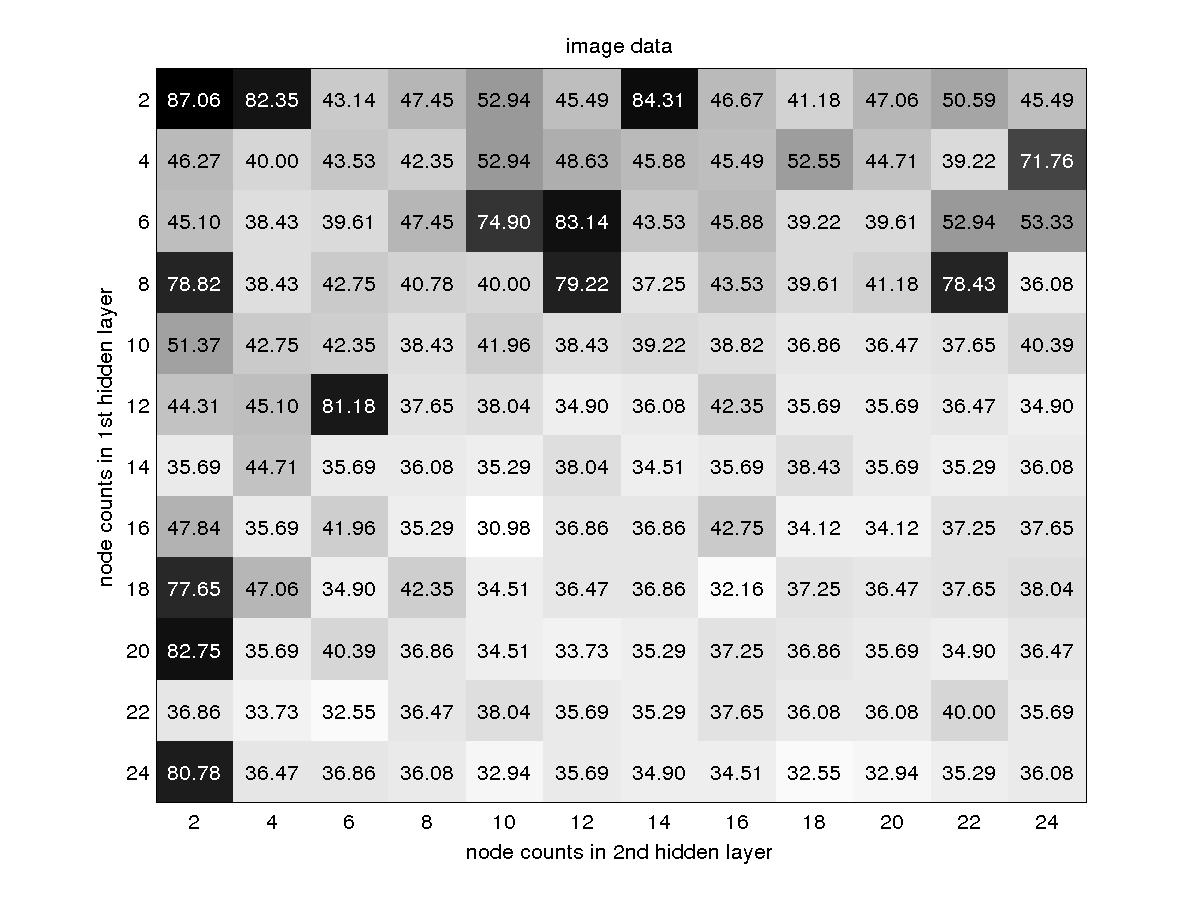
\includegraphics[scale=0.2]{pics/imagedata/image data_validationerror}
\end{subfigure}
\begin{subfigure}{.5\textwidth}
\caption{confusion matrix of\\ train-data}
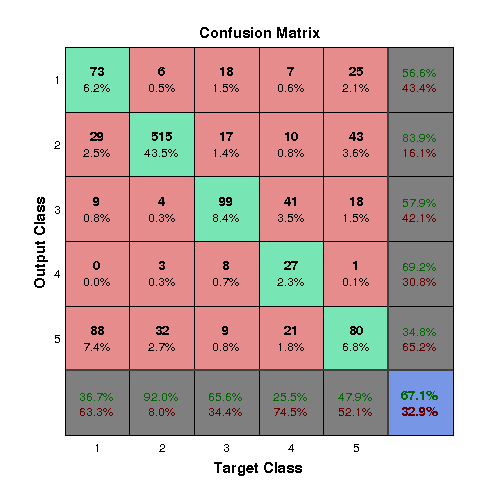
\includegraphics[scale=0.5]{./pics/imagedata/_16_10/_16_10_epoch_Inf_confusiontrain}
\end{subfigure}
\end{figure}

\begin{figure}[!ht]
\begin{subfigure}{.5\textwidth}
\caption{confusion matrix of\\ validation-data}
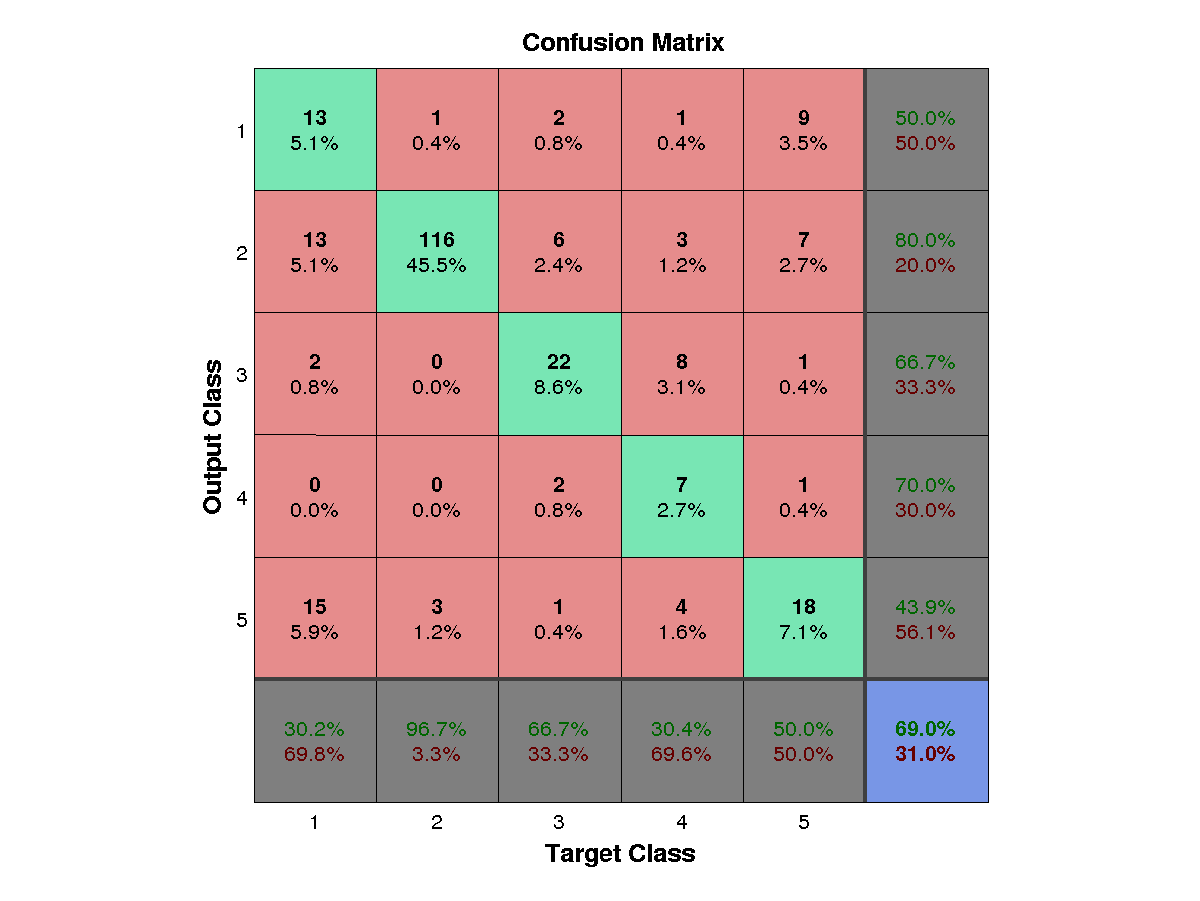
\includegraphics[scale=0.4]{./pics/imagedata/_16_10/_16_10_epoch_Inf_confusion}
\end{subfigure}
\begin{subfigure}{.5\textwidth}
\caption{confusion matrix of\\ test-data}
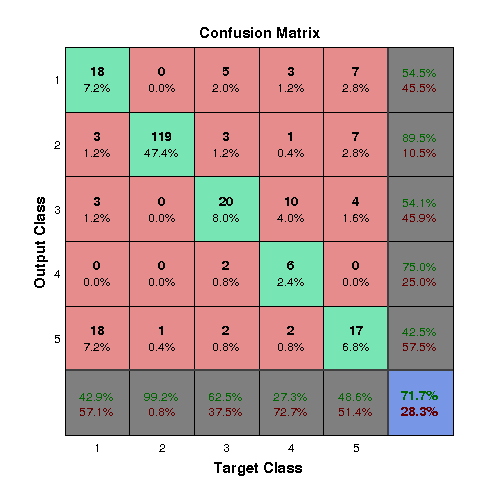
\includegraphics[scale=0.4]{./pics/imagedata/_16_10/_16_10_epoch_Inf_confusiontest}
\end{subfigure}
\end{figure}

\myparagraph{Observations}

\begin{itemize}
  \item The classification accuracy of \~69\% is achieved on validation data for the model complexity of hiddenlayer-1 nodes = 16, hiddenlayer-2 nodes = 10.
  \item The miss percentage seems to increase while adding mode nodes in the hidden layers, as shown in the miss percentage table plot.
  \item We employed min-max normalization in the columns of given features, which did not increase the performance of the trained model. 
  \item Since, the class2 features are more (\~800 images), the model is able to learn this particular class confidently and the classification accuracy for class2 is ~95\% on validation data.
  We are able to infer that having more data is key while training neural networks.
  \item As the number of features for other classes are less, the neural network model is not able to draw a decision boundary confidently for the other classes.
\end{itemize}

\newpage
\subsection{Linearly separable data}

The data and the miss percentage obtained for each complexity of the model is shown below. The miss percentage for model complexity is shown as a table plot (The lighter the cell, the better the performance is).\\
The dataset contains 500 points (train = 250, validation = 150, test = 100) in each of 3 classes.

\begin{figure}[!ht]
\begin{subfigure}{.5\textwidth}
  \caption{Plot of the data}
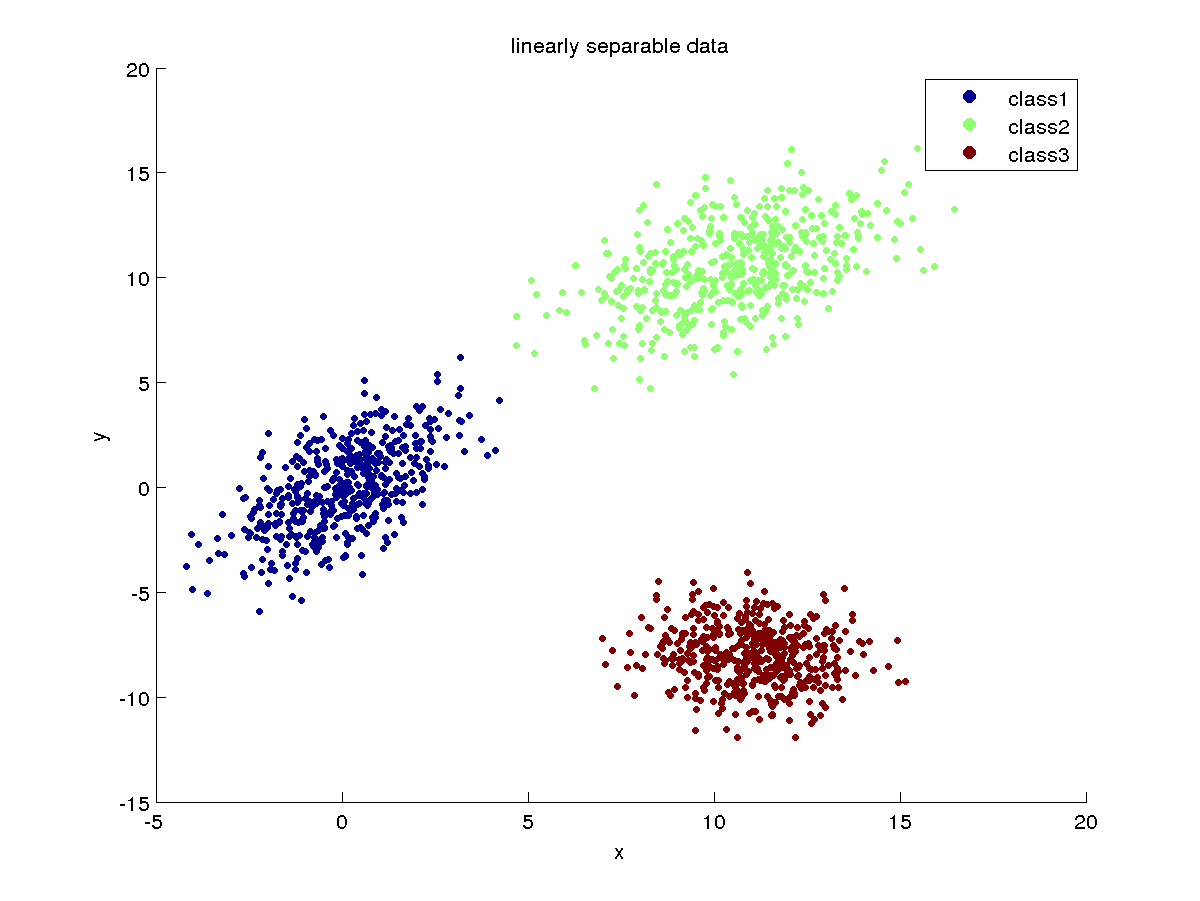
\includegraphics[scale=0.4]{pics/linearlyseparable/dataPlot}
\end{subfigure}
\begin{subfigure}{.5\textwidth}
  \caption{Validation Miss percentage based\\ on model complextites \label{fig:missp}}
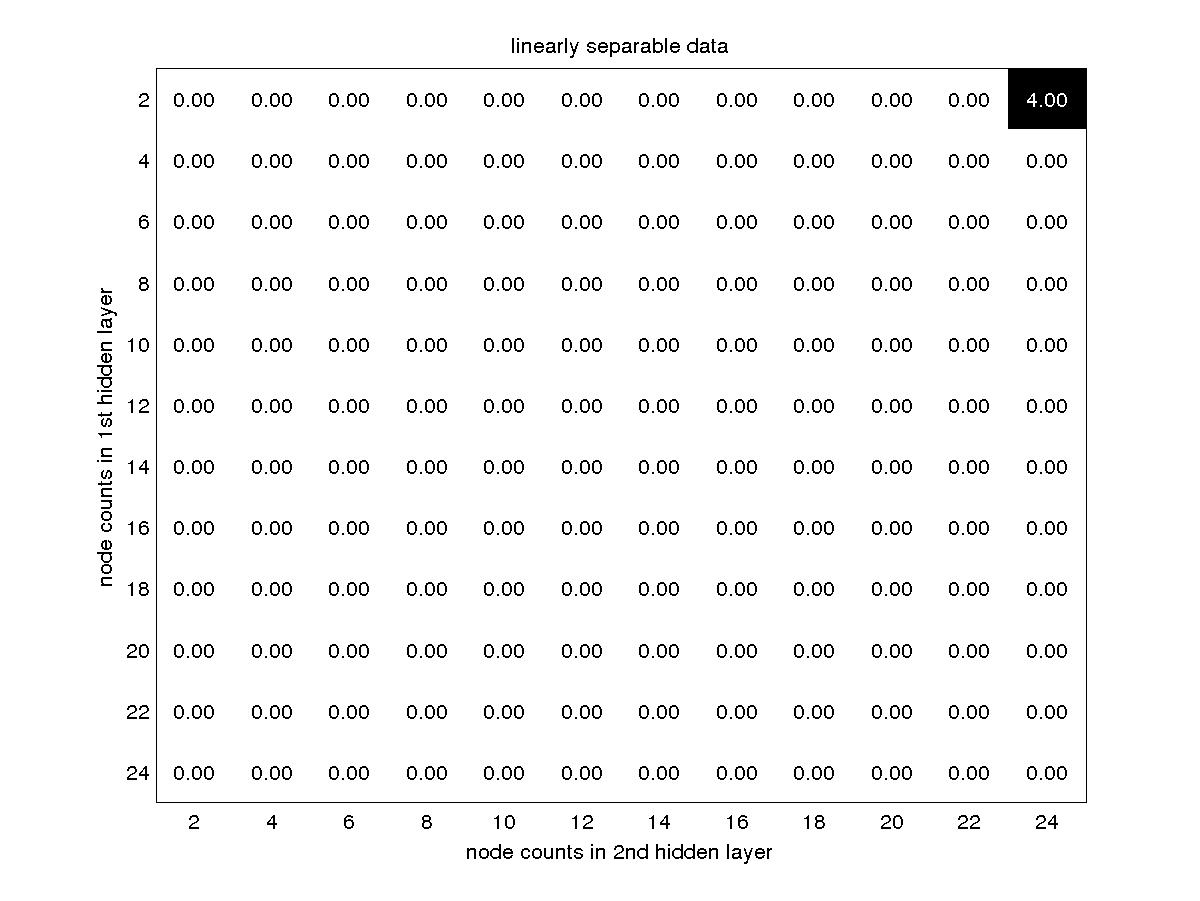
\includegraphics[scale=0.2]{pics/linearlyseparable/linearly separable data_validationerror}
\end{subfigure}
\end{figure}


\subsubsection{MLFFNN with 2 Hidden layers}

\myparagraph{Layer outputs after Training}

\begin{center}
  \begin{longtable}{ c | c | r  }
	\multicolumn{1}{c}{Hidden layer-1 } & 
	\multicolumn{1}{c}{Hidden layer-2 } & 
	\multicolumn{1}{c}{Output layer } \\
    \hline
    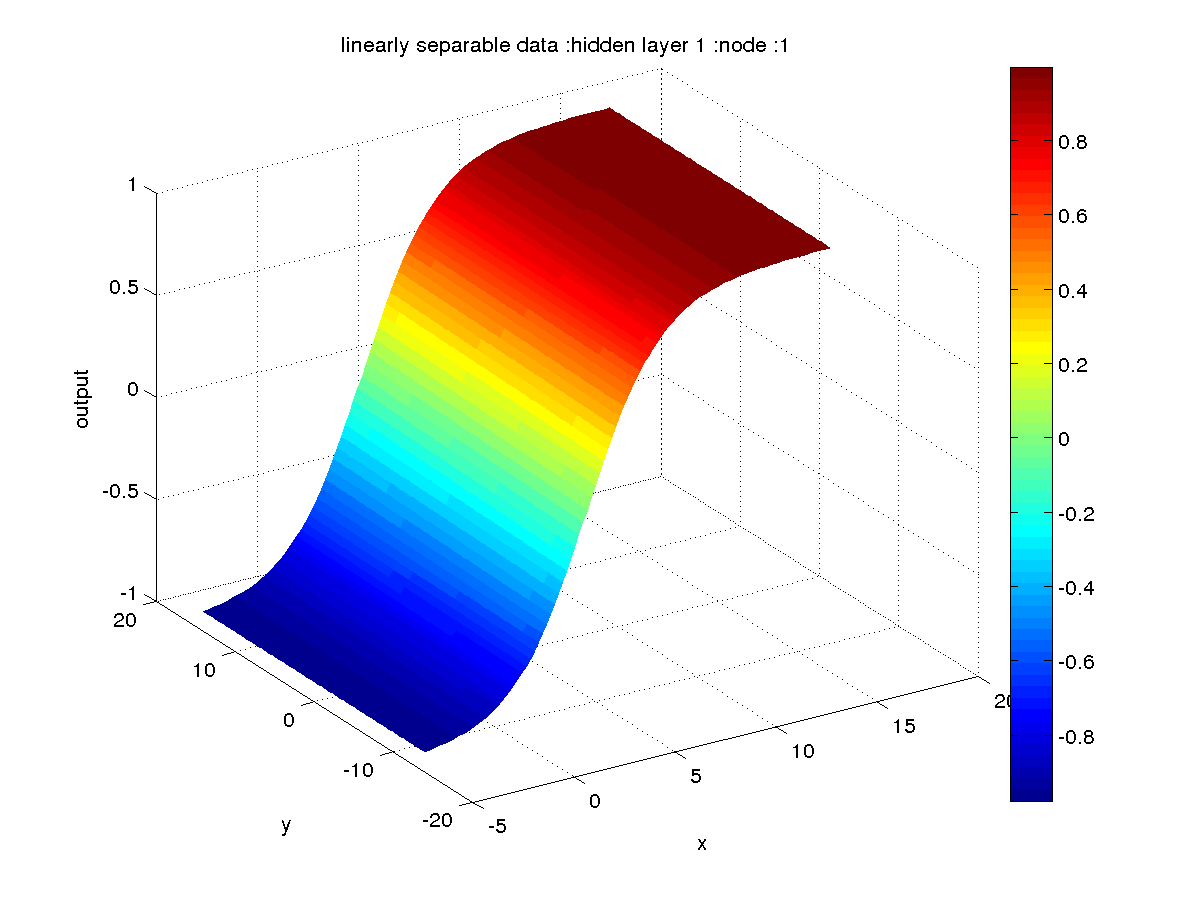
\includegraphics[scale=0.25]{./pics/linearlyseparable/_2_2/_2_2_epoch_Inf_hidden layer 1 :1}  & 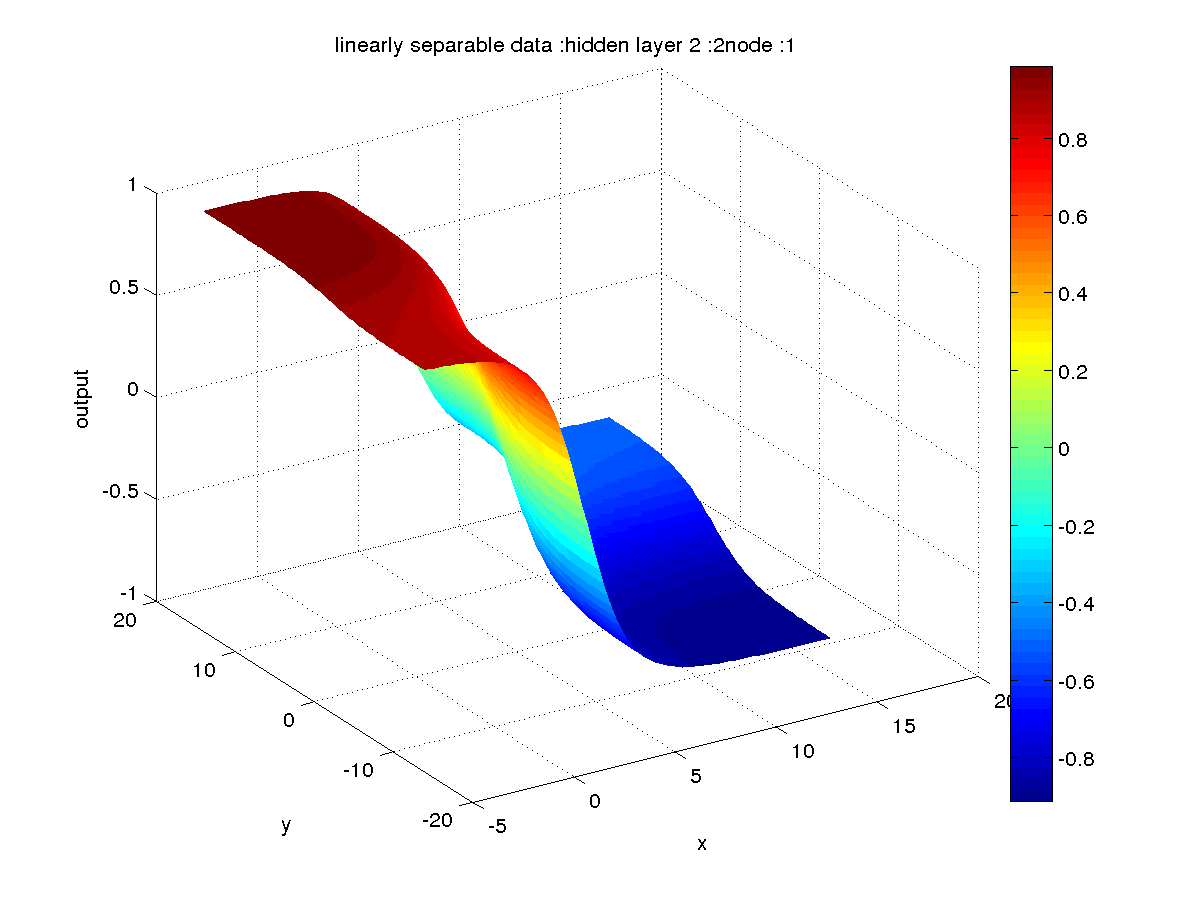
\includegraphics[scale=0.25]{./pics/linearlyseparable/_2_2/_2_2_epoch_Inf_hidden layer 2 :21} & 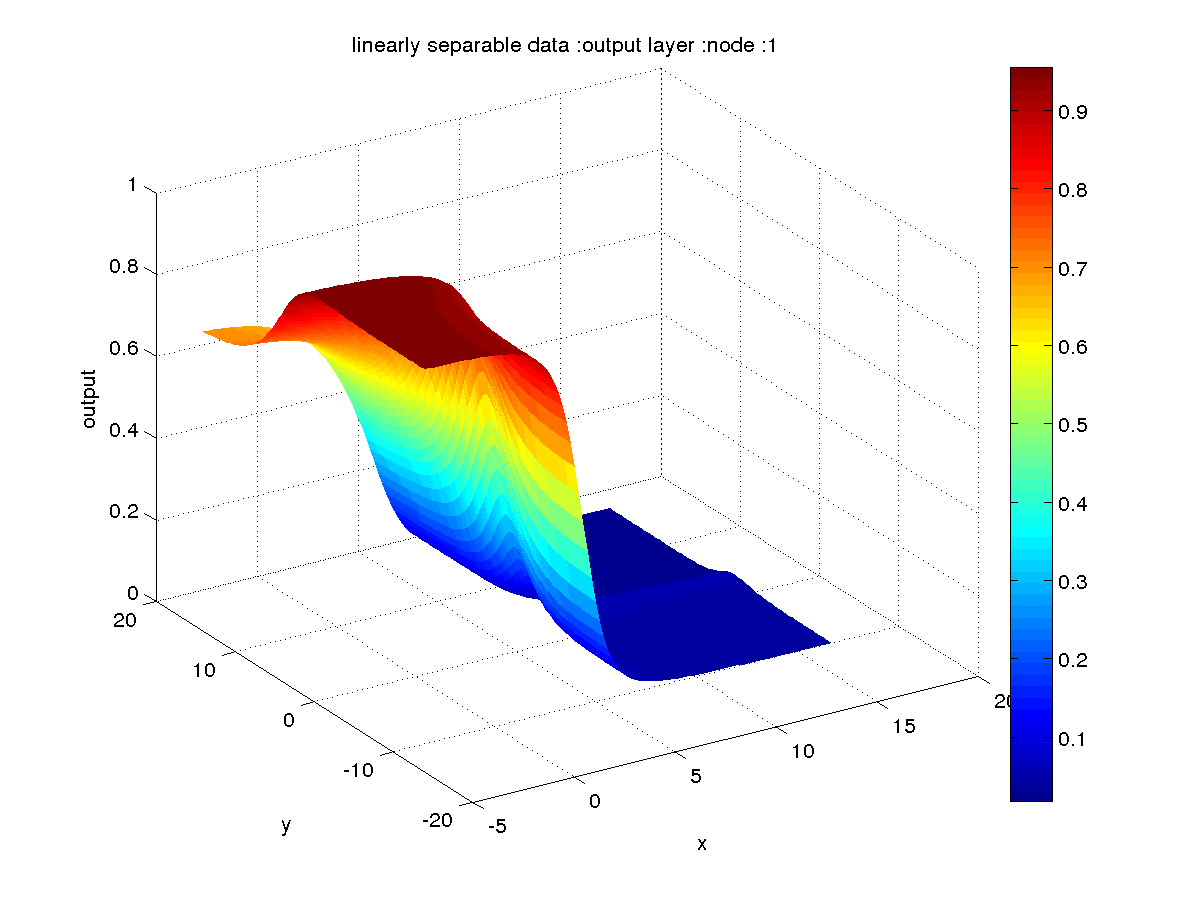
\includegraphics[scale=0.25]{./pics/linearlyseparable/_2_2/_2_2_epoch_Inf_output layer :1}\\ 
     &  & 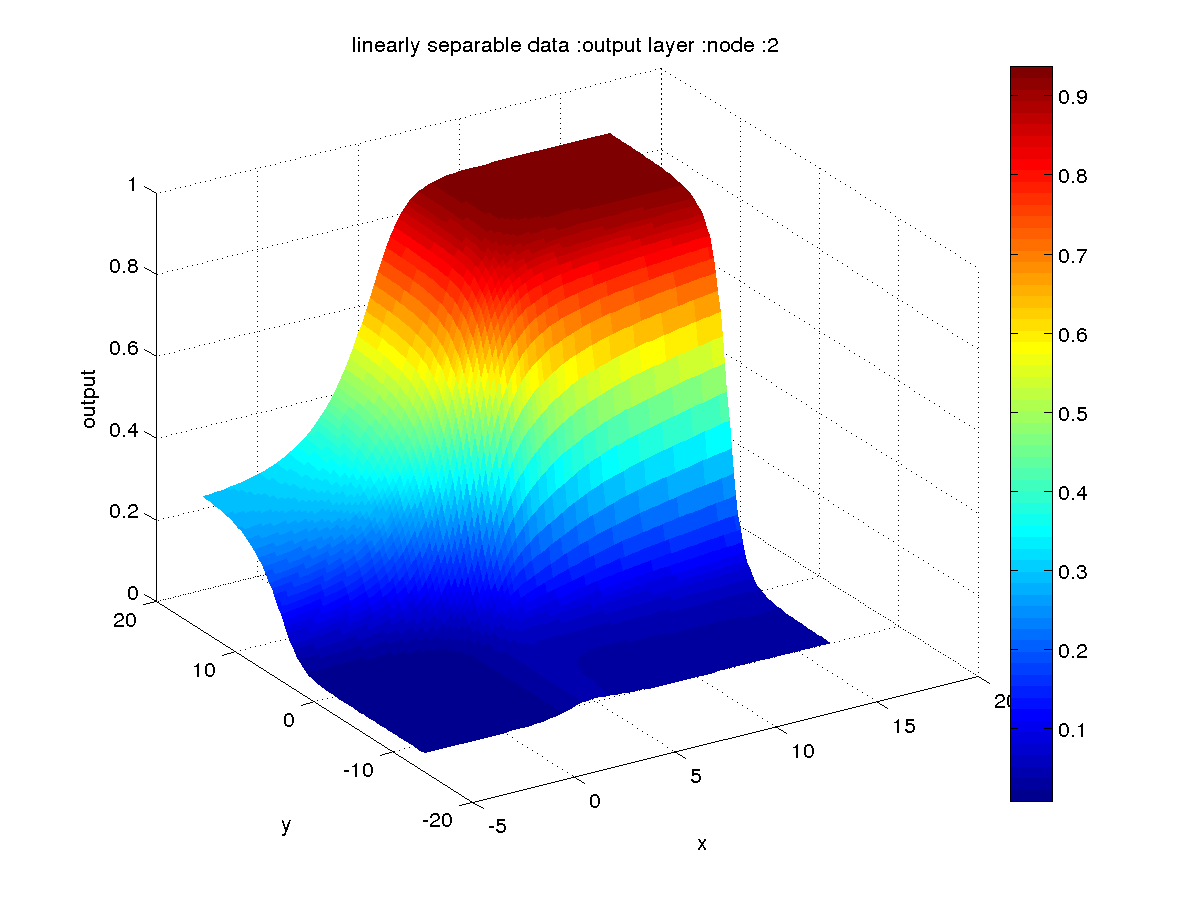
\includegraphics[scale=0.25]{./pics/linearlyseparable/_2_2/_2_2_epoch_Inf_output layer :2} \\ 
    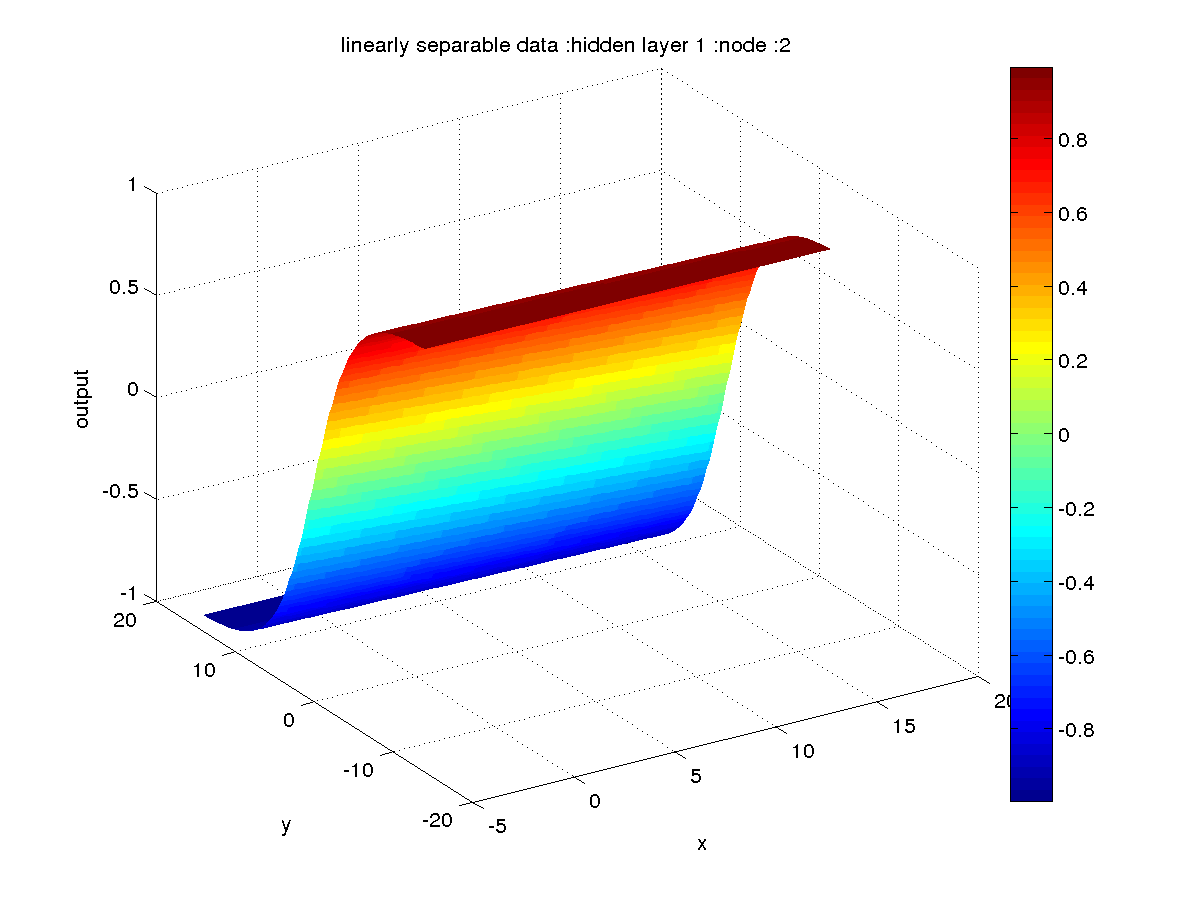
\includegraphics[scale=0.25]{./pics/linearlyseparable/_2_2/_2_2_epoch_Inf_hidden layer 1 :2} & 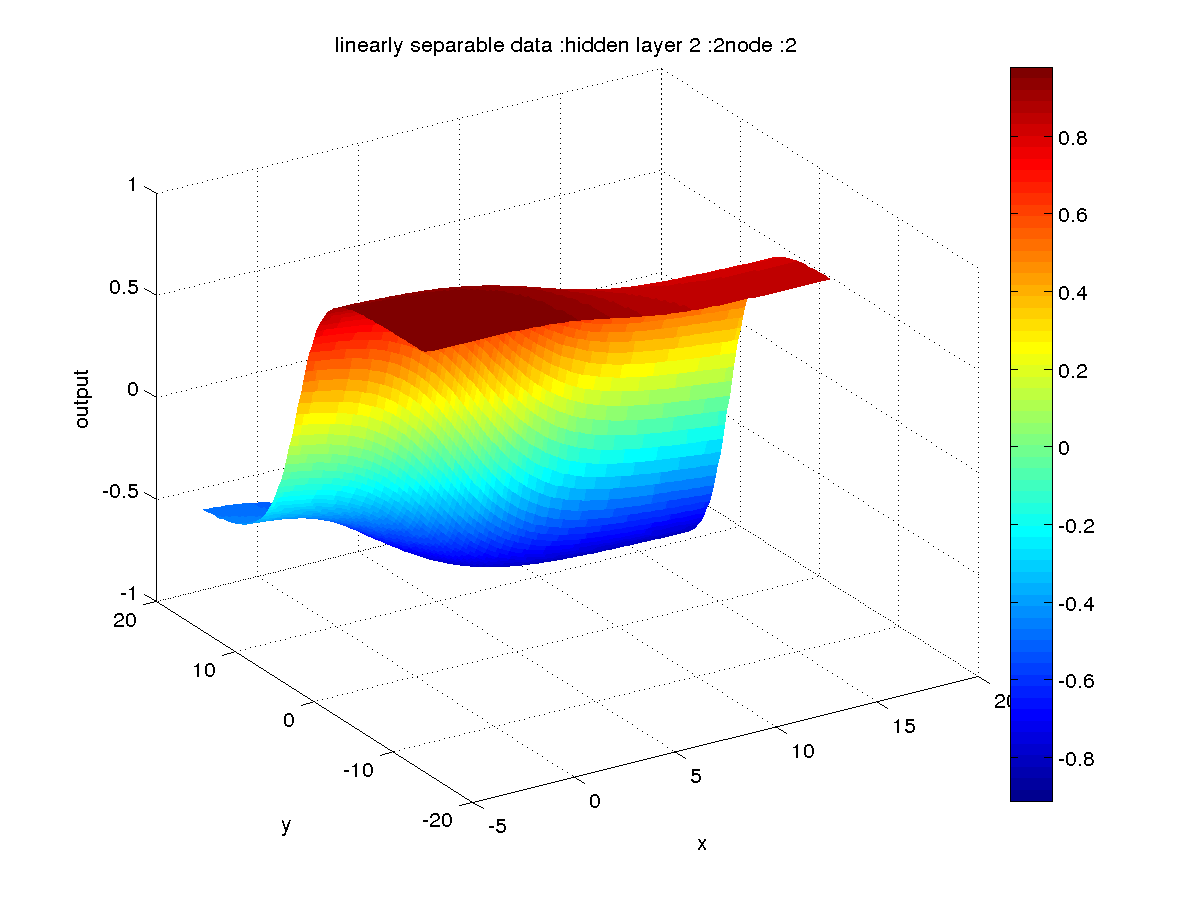
\includegraphics[scale=0.25]{./pics/linearlyseparable/_2_2/_2_2_epoch_Inf_hidden layer 2 :22} & 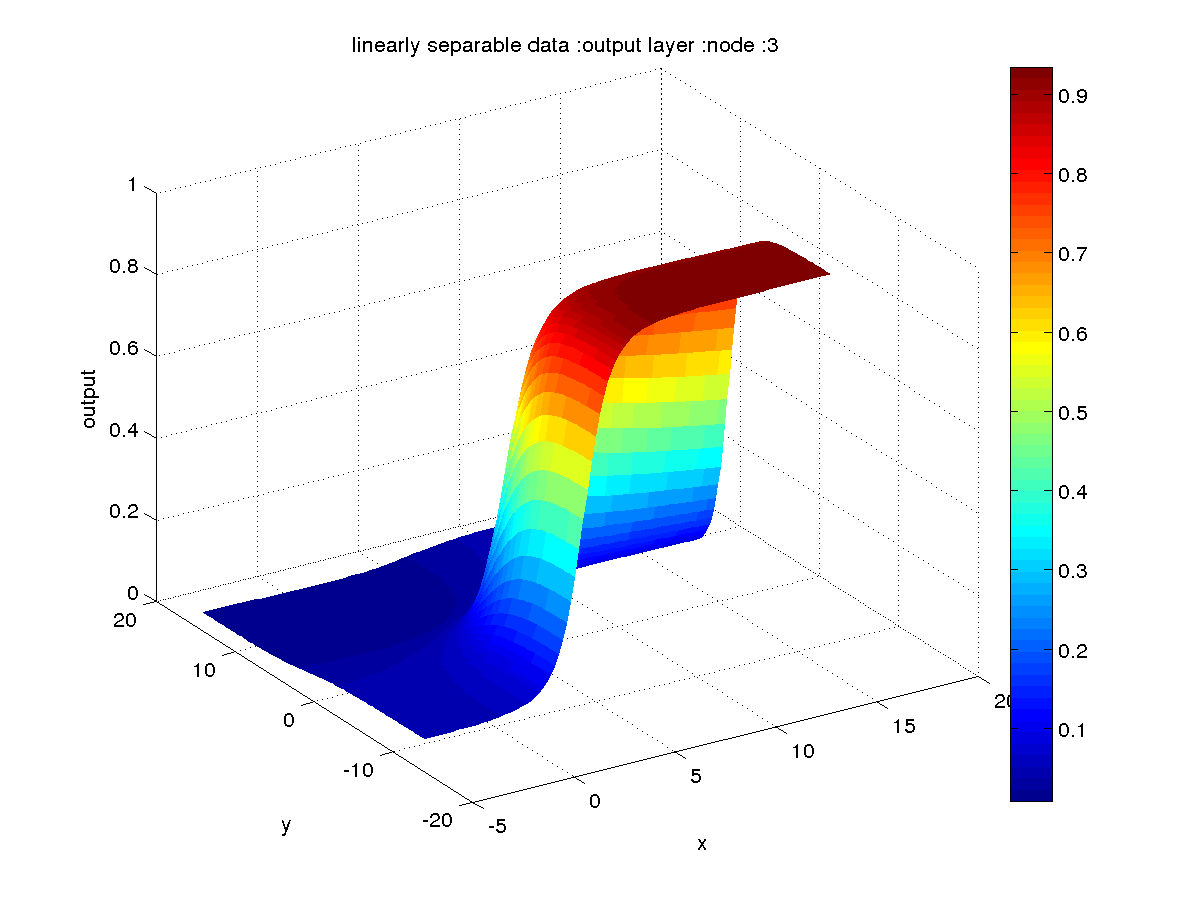
\includegraphics[scale=0.25]{./pics/linearlyseparable/_2_2/_2_2_epoch_Inf_output layer :3}\\
    \hline
  \end{longtable}
\end{center}

\myparagraph{Decision boundary \& Confusion matrix}

\begin{figure}[!ht]
\begin{subfigure}{.3\textwidth}
\caption{Decision boundary plot}
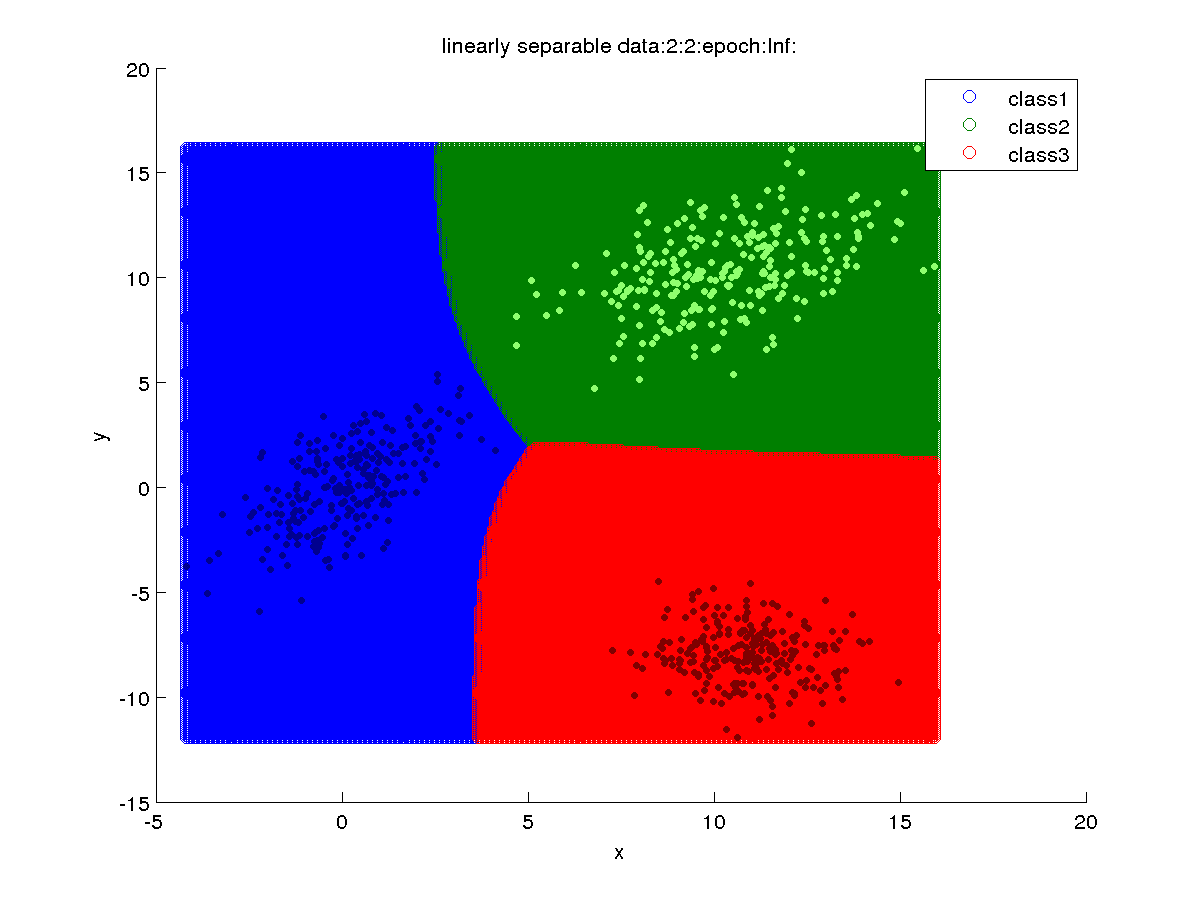
\includegraphics[scale=0.3]{./pics/linearlyseparable/_2_2/_2_2_epoch_Inf_decisionBoundary}
\end{subfigure}
\begin{subfigure}{.3\textwidth}
\caption{combined output\\ of final layer nodes}
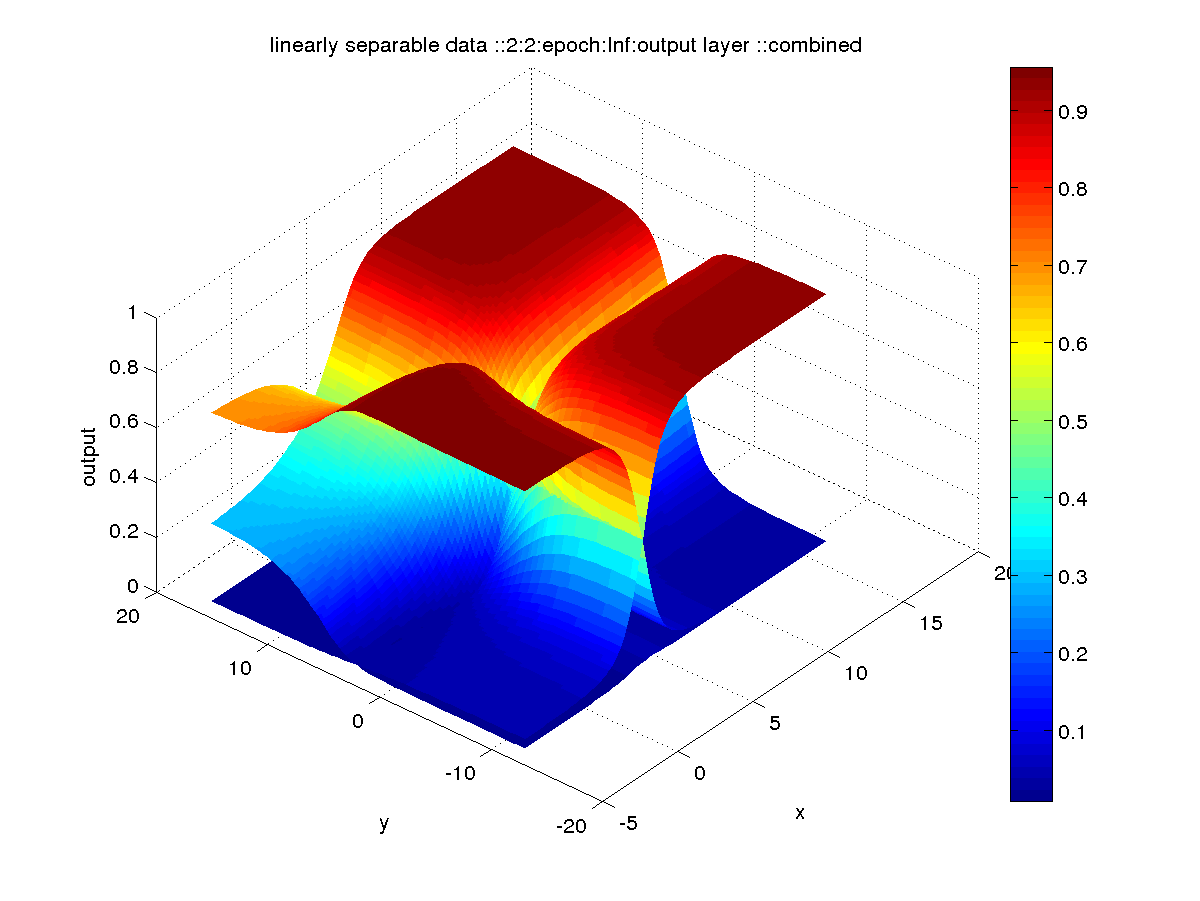
\includegraphics[scale=0.3]{./pics/linearlyseparable/_2_2/_2_2_epoch_Inf_output layer :_combined}
\end{subfigure}
\begin{subfigure}{.3\textwidth}
\caption{confusion matrix \\ of train data}
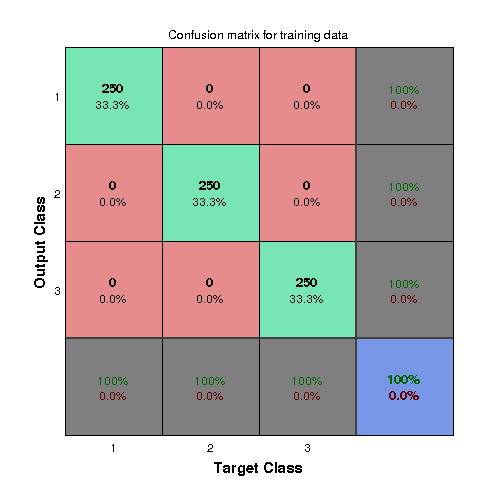
\includegraphics[scale=0.3]{./pics/linearlyseparable/_2_2/_2_2_epoch_Inf_confusiontrain}
\end{subfigure}
\end{figure}

\begin{figure}[!ht]
\begin{subfigure}{.5\textwidth}
\caption{confusion matrix \\ of validation data}
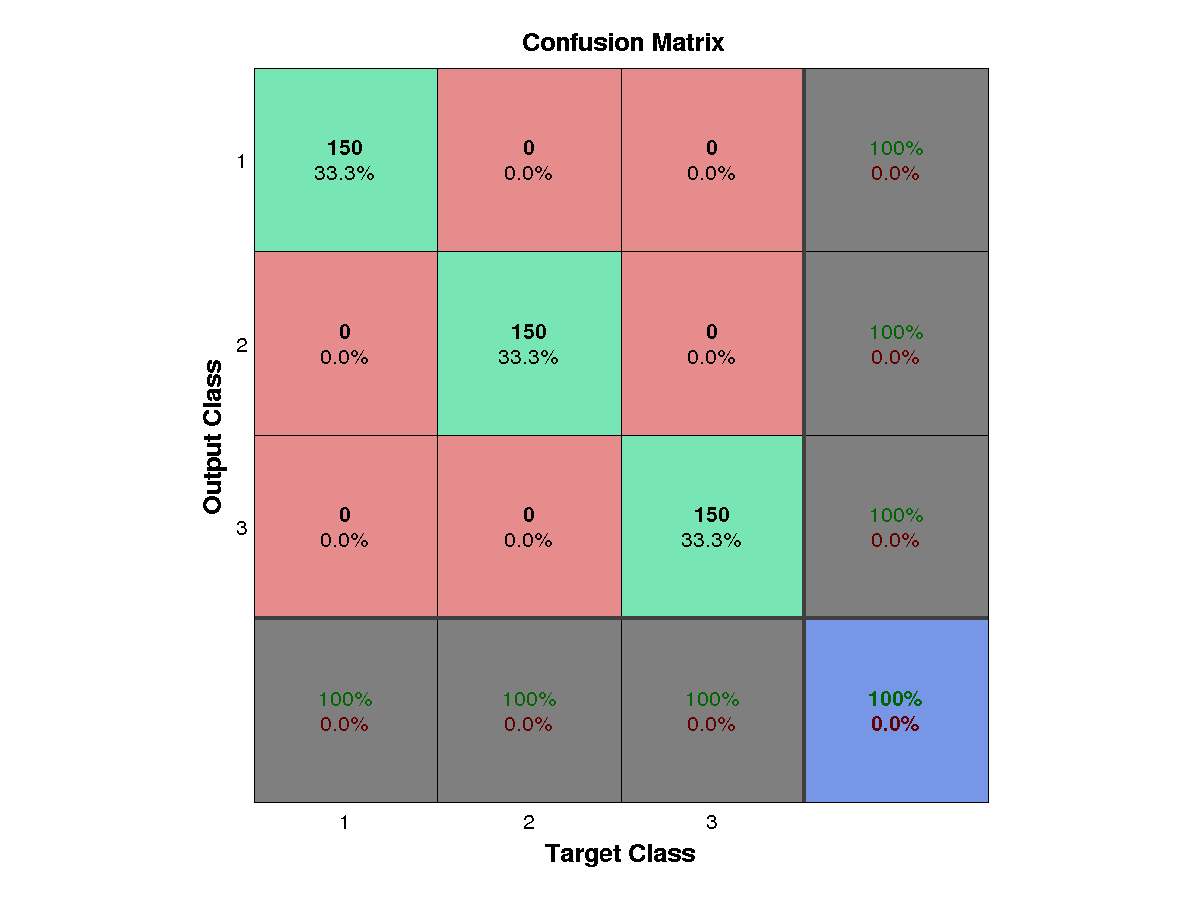
\includegraphics[scale=0.4]{./pics/linearlyseparable/_2_2/_2_2_epoch_Inf_confusion}
\end{subfigure}
\begin{subfigure}{.5\textwidth}
\caption{confusion matrix \\ of test data}
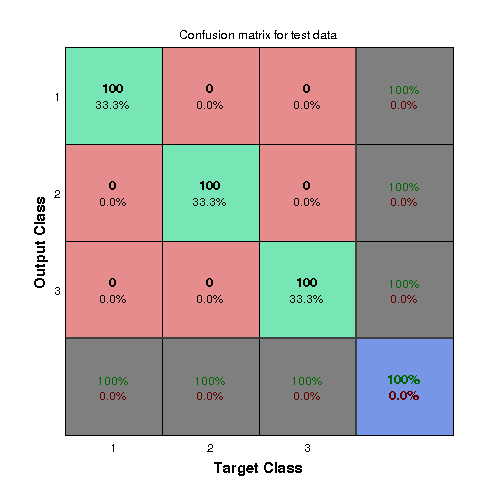
\includegraphics[scale=0.4]{./pics/linearlyseparable/_2_2/_2_2_epoch_Inf_confusiontest}
\end{subfigure}
\end{figure}

\myparagraph{Observations}

\begin{itemize}
  \item Since, the dataset is a linearly separable one, the less complex model is able to achieve 100\% efficiency. 
  \item As seen in the \textit{Miss percentage image}, almost all of the models are able to give 0\% error rate. hence, we choose a simple model with node counts of hidden layer1 = 2, hidden layer2 = 2. This model converges to best performace in 125 epochs.
  \item As shown in the decision boundary plot, the model is able to easily separate the data. Since, the model hidden layers are made up of $tansig$ non-linearities, the decision boundary is a combination of non-linearities from hidden layers.   
\end{itemize}

\newpage
\subsection{Non-linearly separable data}
The visual plot and validation data miss-percentage box plot are shown below.\\
The dataset contains 300 points (train = 150, validation = 90, test = 60) of class1, \\ 
600 points (train = 300, validation = 180, test = 120) of class2, \\
800 points (train = 400, validation = 240, test = 160) of class3.\\

\begin{figure}[!ht]
\begin{subfigure}{.5\textwidth}
  \caption{Plot of the data}
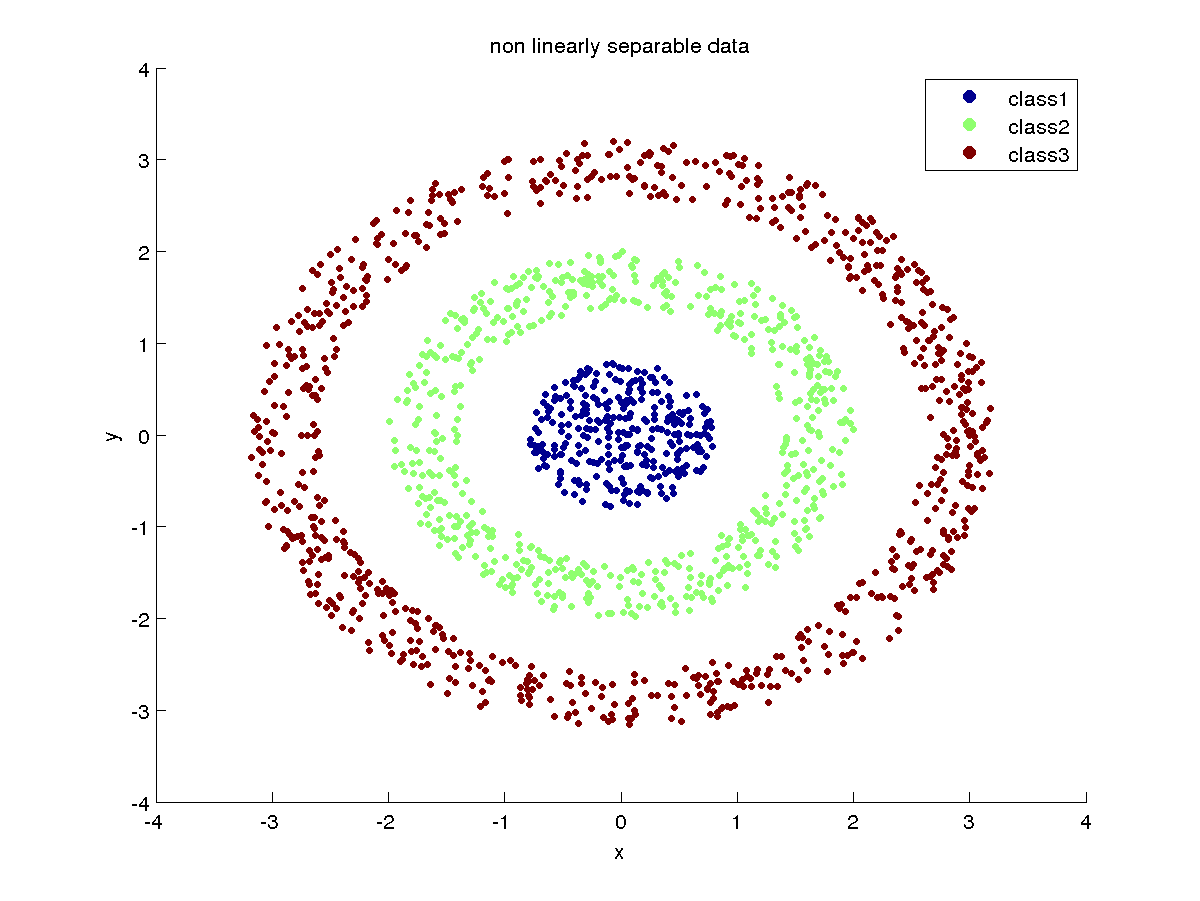
\includegraphics[scale=0.4]{pics/nonlinearlyseparable/dataPlot}
\end{subfigure}
\begin{subfigure}{.5\textwidth}
  \caption{Validation Miss percentage based\\ on model complextites}
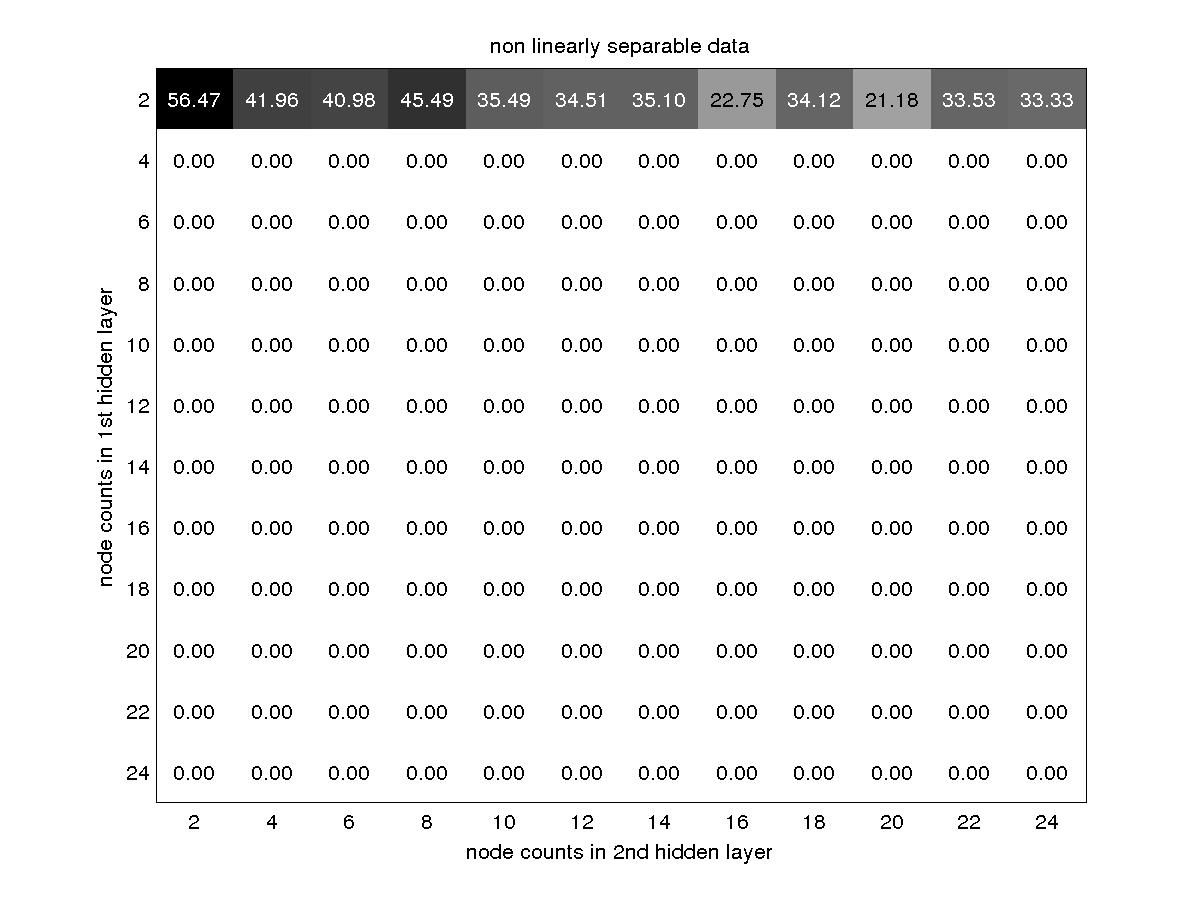
\includegraphics[scale=0.2]{pics/nonlinearlyseparable/non linearly separable data_validationerror}
\end{subfigure}
\end{figure}

Based on the  validation data miss percentage plot, the model of (hiddenlayer1 \#nodes = 4, hiddenlayer2 \#nodes = 2) is chosen as the best model.

\newpage
\subsubsection{MLFFNN with 2 Hidden layers}

\myparagraph{After 1 epoch}

\begin{center}
  \begin{longtable}{ c | c | r }
	\multicolumn{1}{c}{Hidden layer-1 } & 
	\multicolumn{1}{c}{Hidden layer-2 } & 
	\multicolumn{1}{c}{Output layer } \\
    \hline
    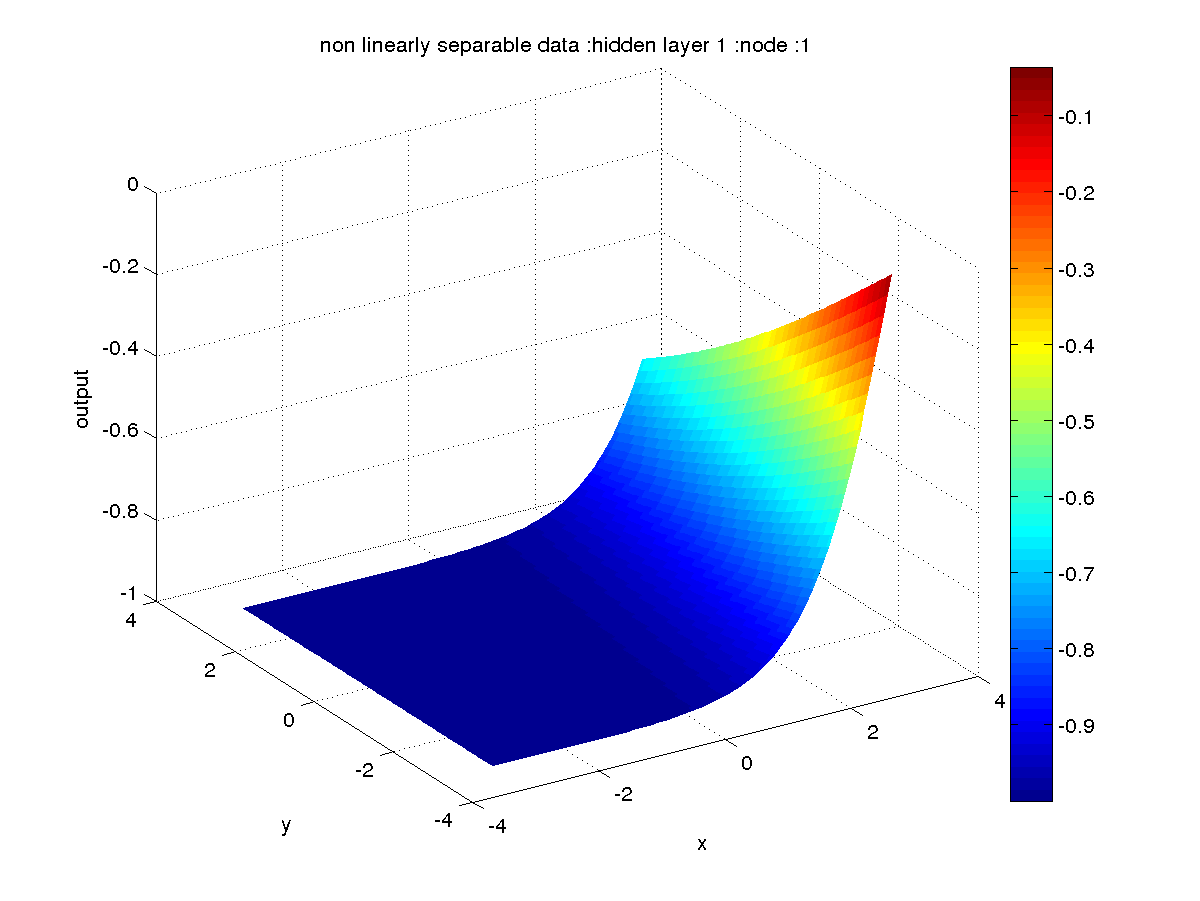
\includegraphics[scale=0.25]{./pics/nonlinearlyseparable/_4_2/_4_2_epoch_1_hidden layer 1 :1}  & 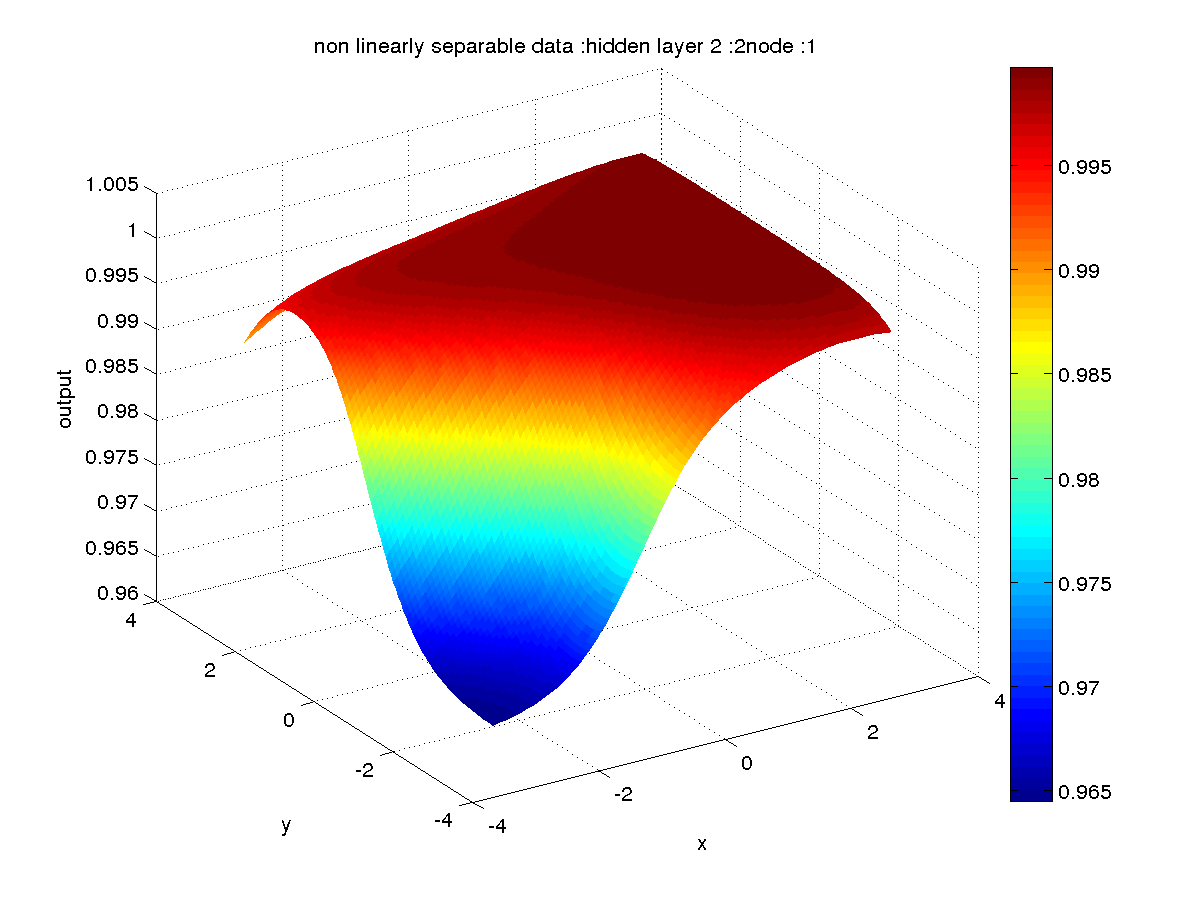
\includegraphics[scale=0.25]{./pics/nonlinearlyseparable/_4_2/_4_2_epoch_1_hidden layer 2 :21} & 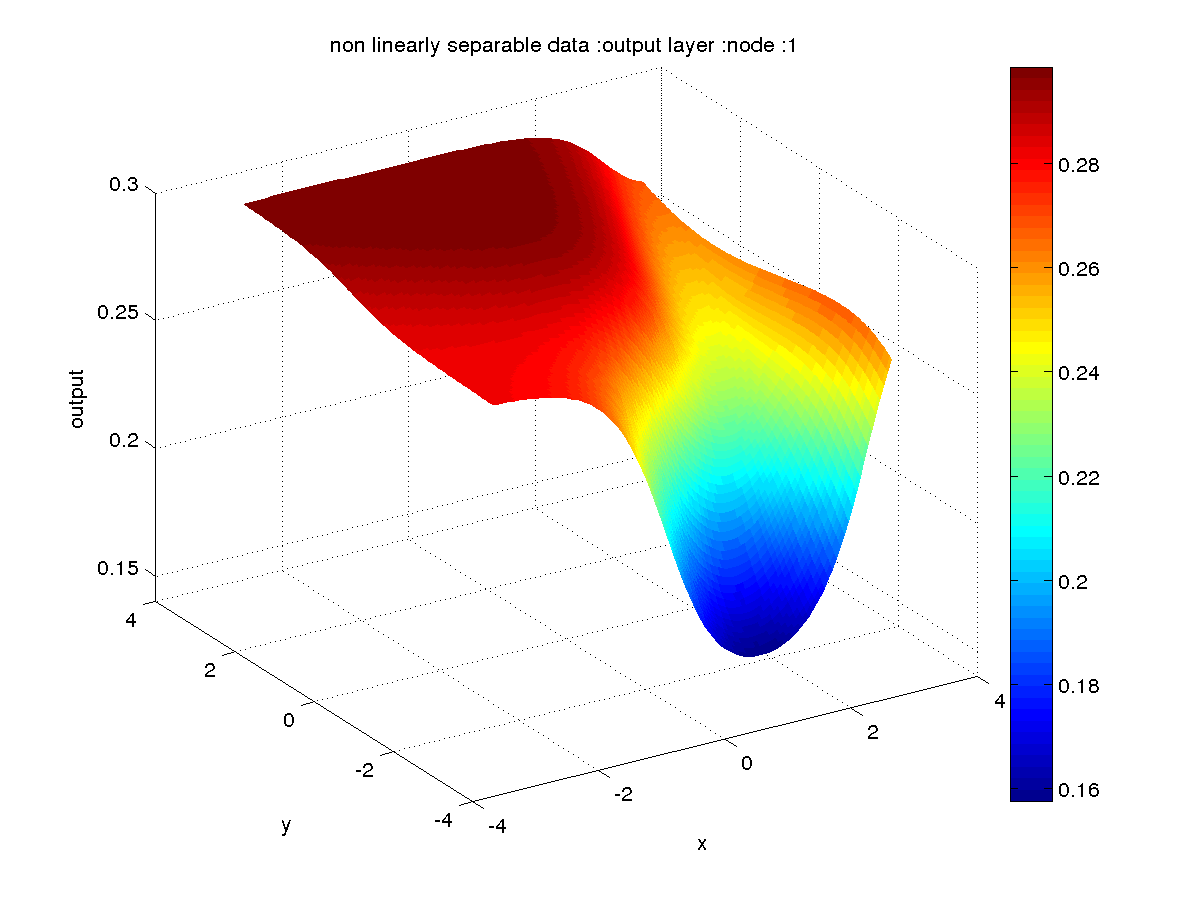
\includegraphics[scale=0.25]{./pics/nonlinearlyseparable/_4_2/_4_2_epoch_1_output layer :1}\\ 
    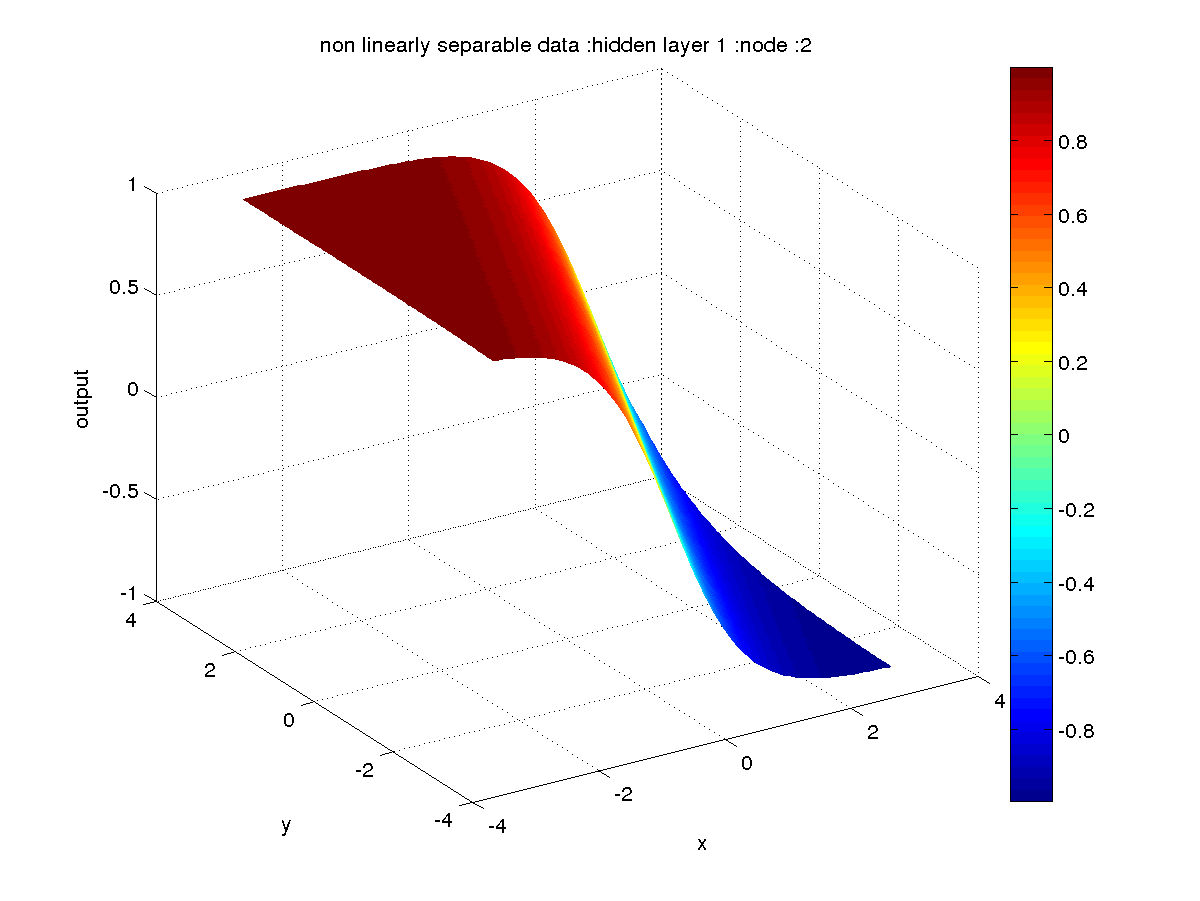
\includegraphics[scale=0.25]{./pics/nonlinearlyseparable/_4_2/_4_2_epoch_1_hidden layer 1 :2} &  & 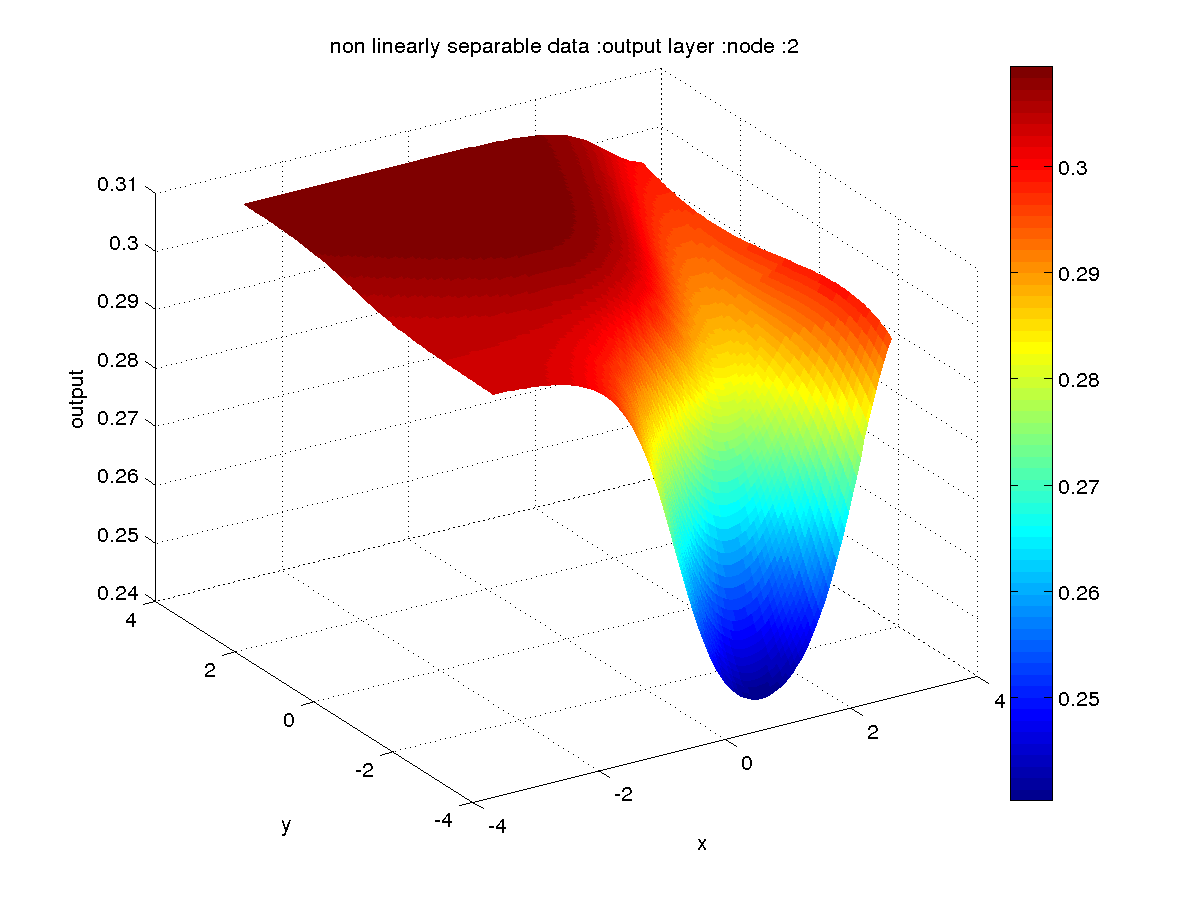
\includegraphics[scale=0.25]{./pics/nonlinearlyseparable/_4_2/_4_2_epoch_1_output layer :2} \\ 
    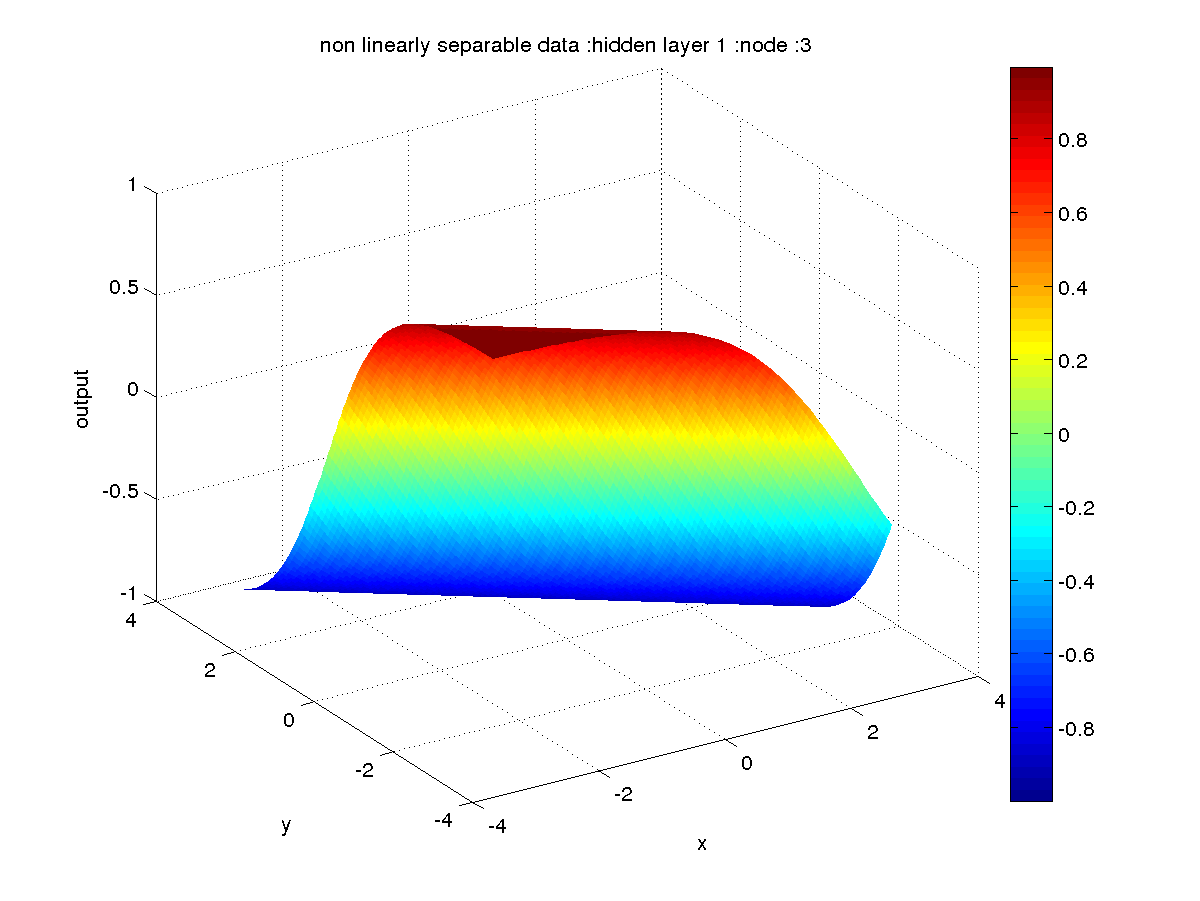
\includegraphics[scale=0.25]{./pics/nonlinearlyseparable/_4_2/_4_2_epoch_1_hidden layer 1 :3} & 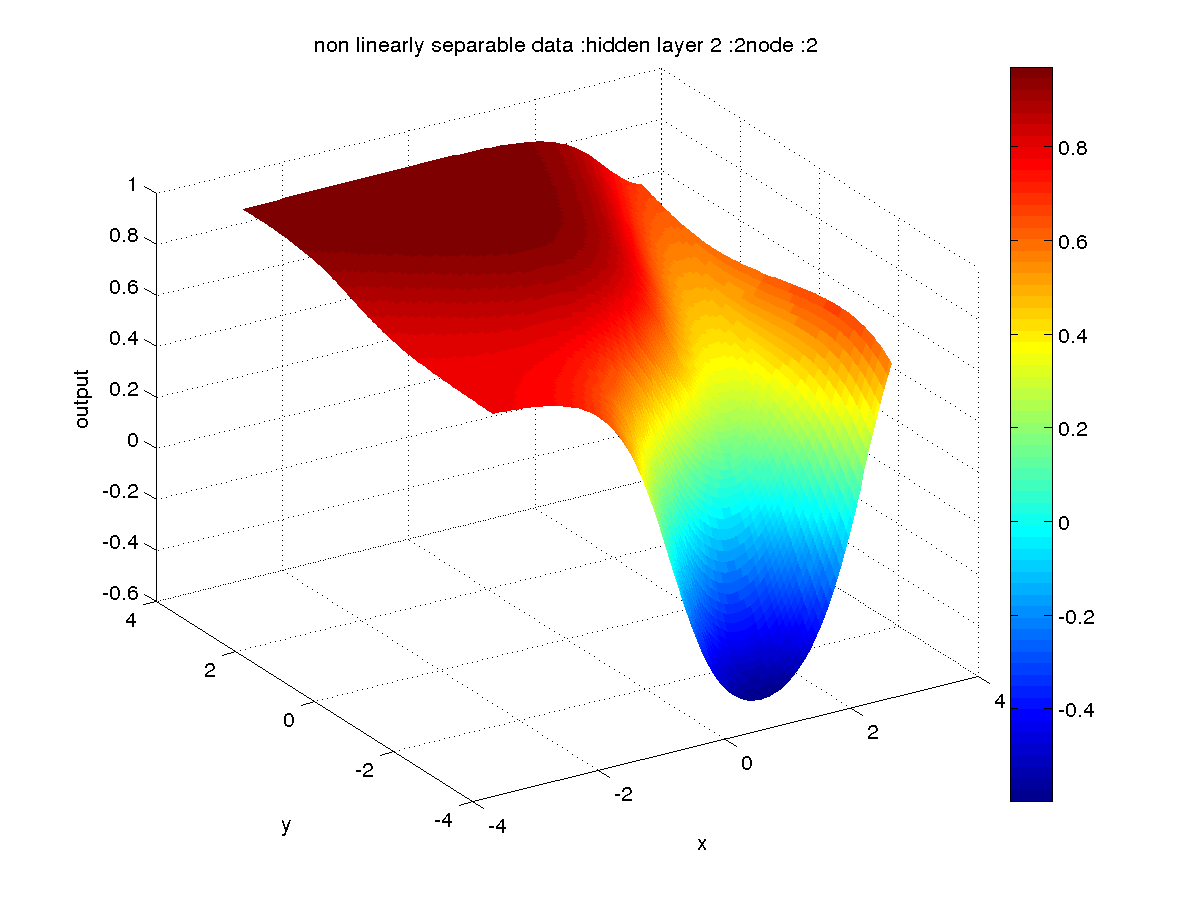
\includegraphics[scale=0.25]{./pics/nonlinearlyseparable/_4_2/_4_2_epoch_1_hidden layer 2 :22} & 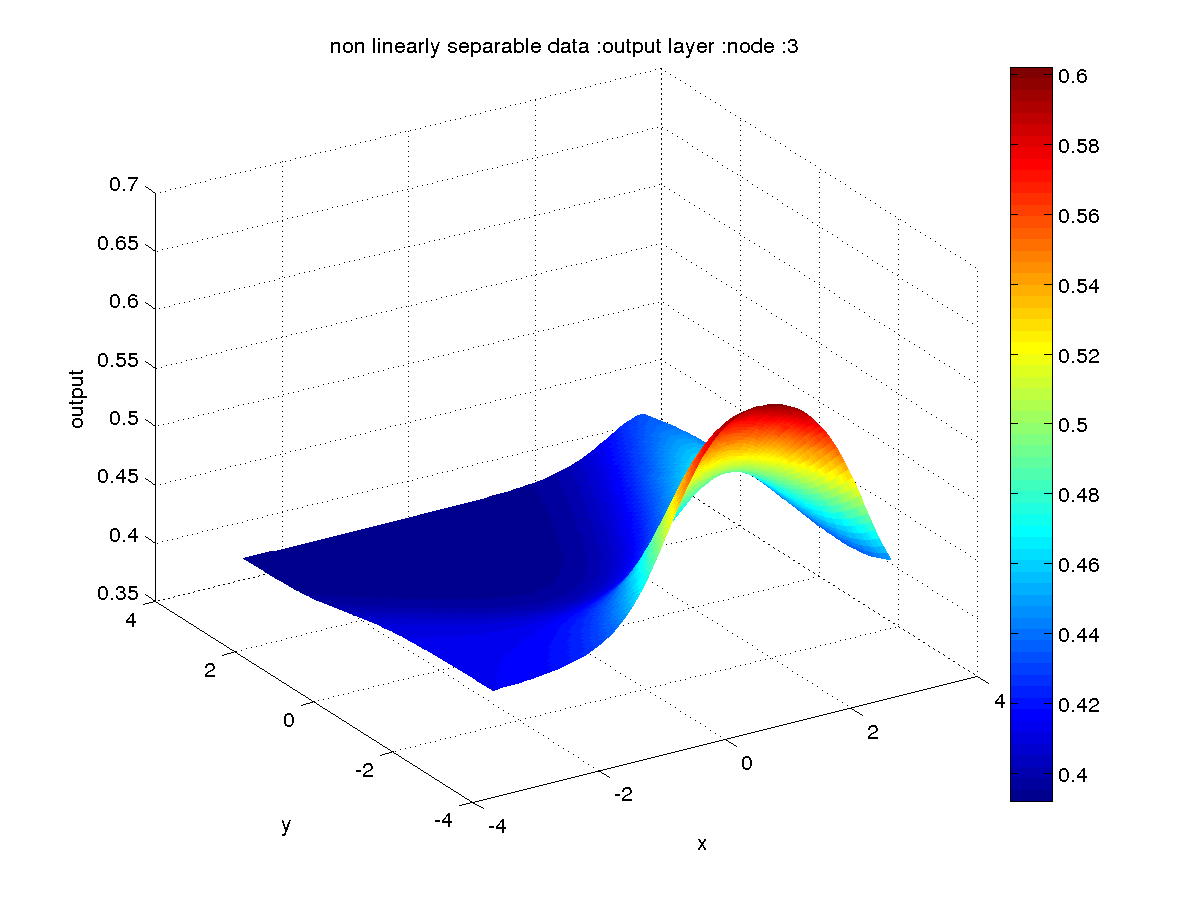
\includegraphics[scale=0.25]{./pics/nonlinearlyseparable/_4_2/_4_2_epoch_1_output layer :3}\\
    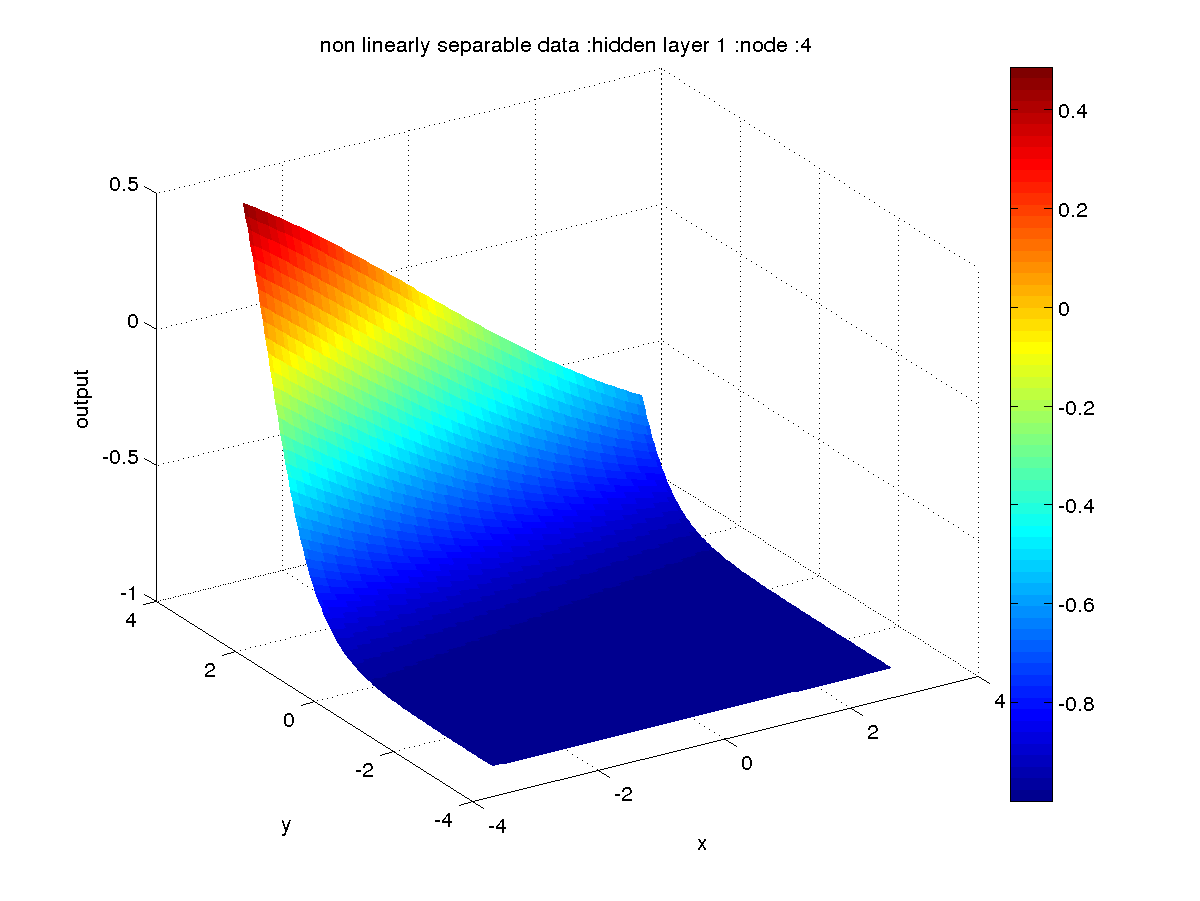
\includegraphics[scale=0.25]{./pics/nonlinearlyseparable/_4_2/_4_2_epoch_1_hidden layer 1 :4} &  & \\ 
    \hline
  \end{longtable}
\end{center}

\begin{figure}[!ht]
\begin{subfigure}{.3\textwidth}
\caption{Decision boundary plot}
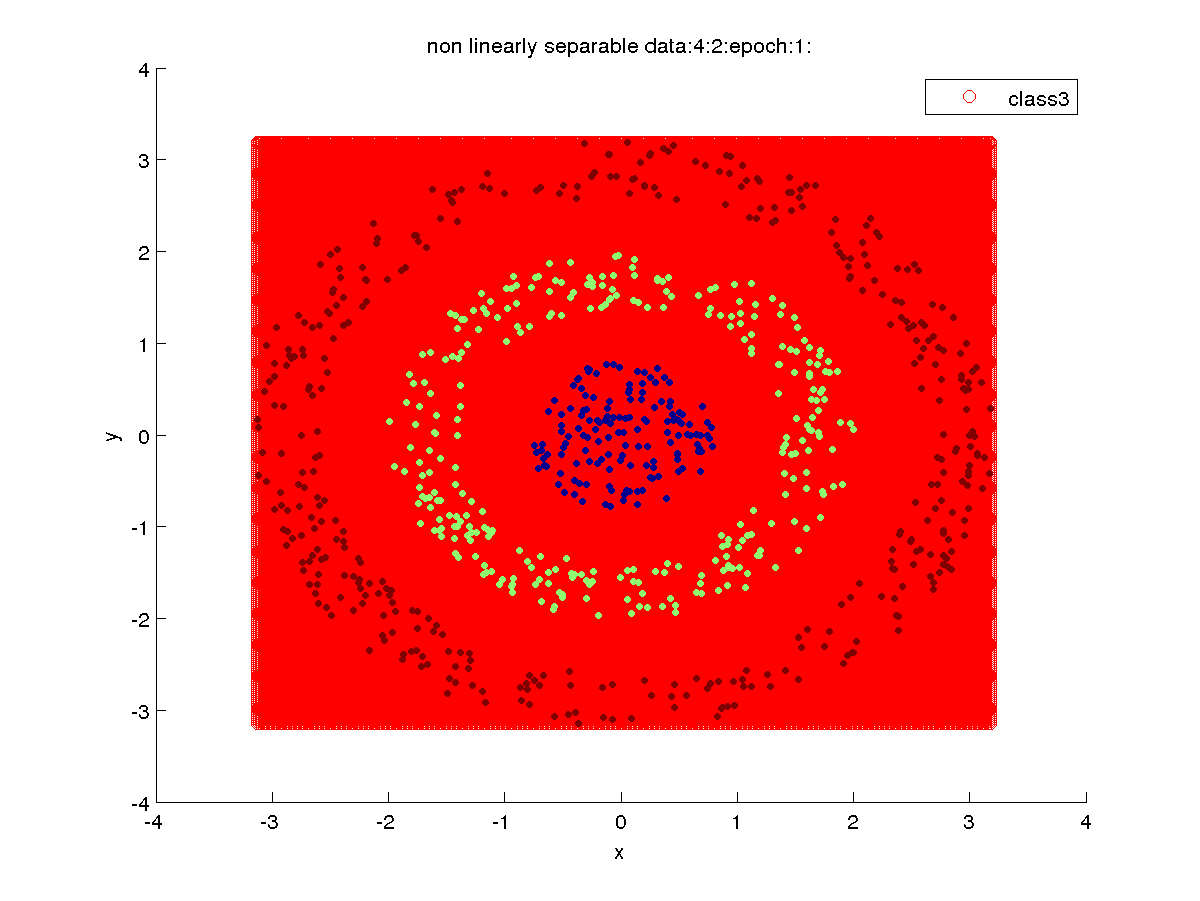
\includegraphics[scale=0.3]{./pics/nonlinearlyseparable/_4_2/_4_2_epoch_1_decisionBoundary}
\end{subfigure}
\begin{subfigure}{.3\textwidth}
\caption{combined output\\ of final layer nodes}
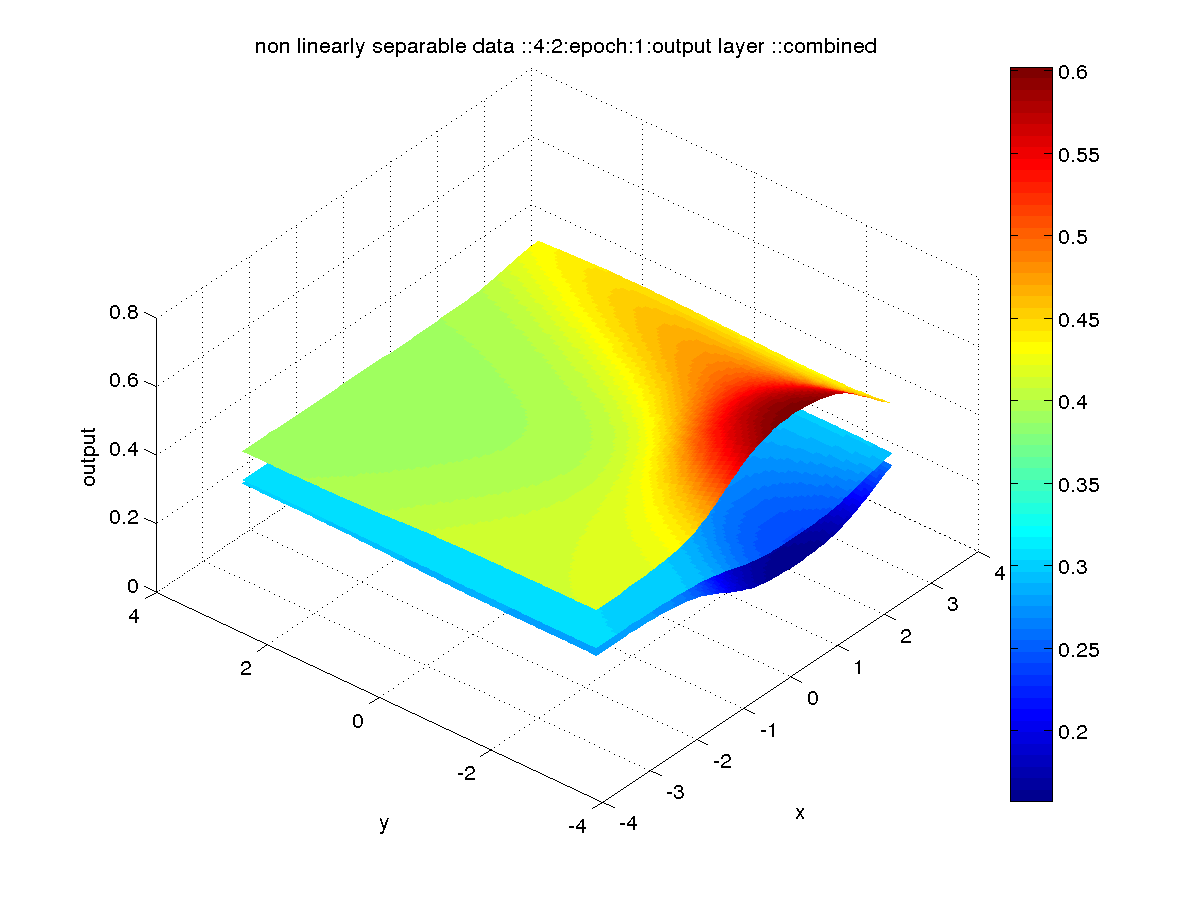
\includegraphics[scale=0.3]{./pics/nonlinearlyseparable/_4_2/_4_2_epoch_1_output layer :_combined}
\end{subfigure}
\begin{subfigure}{.3\textwidth}
\caption{confusion matrix \\ of validation data}
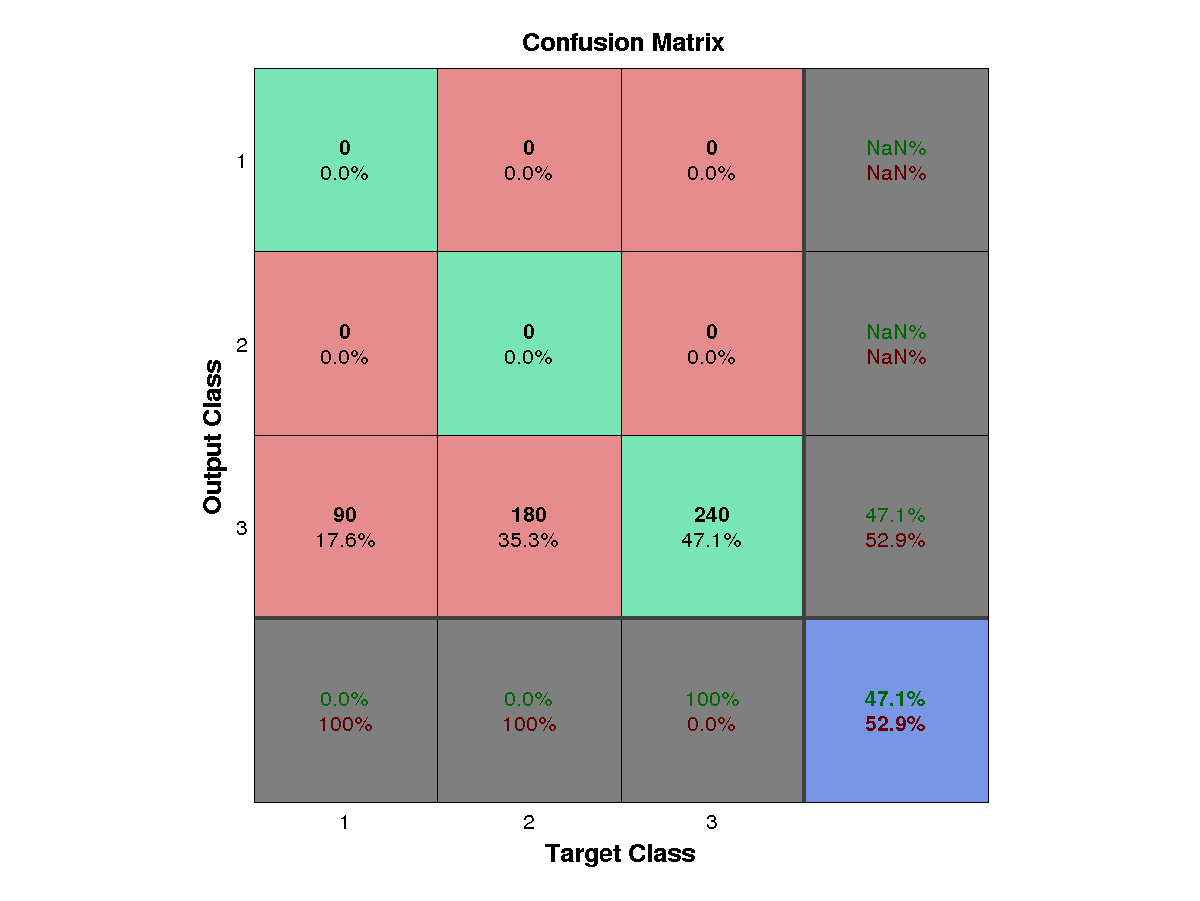
\includegraphics[scale=0.3]{./pics/nonlinearlyseparable/_4_2/_4_2_epoch_1_confusion}
\end{subfigure}
\end{figure}

\newpage
\myparagraph{After 2 epochs}

\begin{center}
  \begin{longtable}{ c | c | r  }
	\multicolumn{1}{c}{Hidden layer-1 } & 
	\multicolumn{1}{c}{Hidden layer-2 } & 
	\multicolumn{1}{c}{Output layer } \\
    \hline
    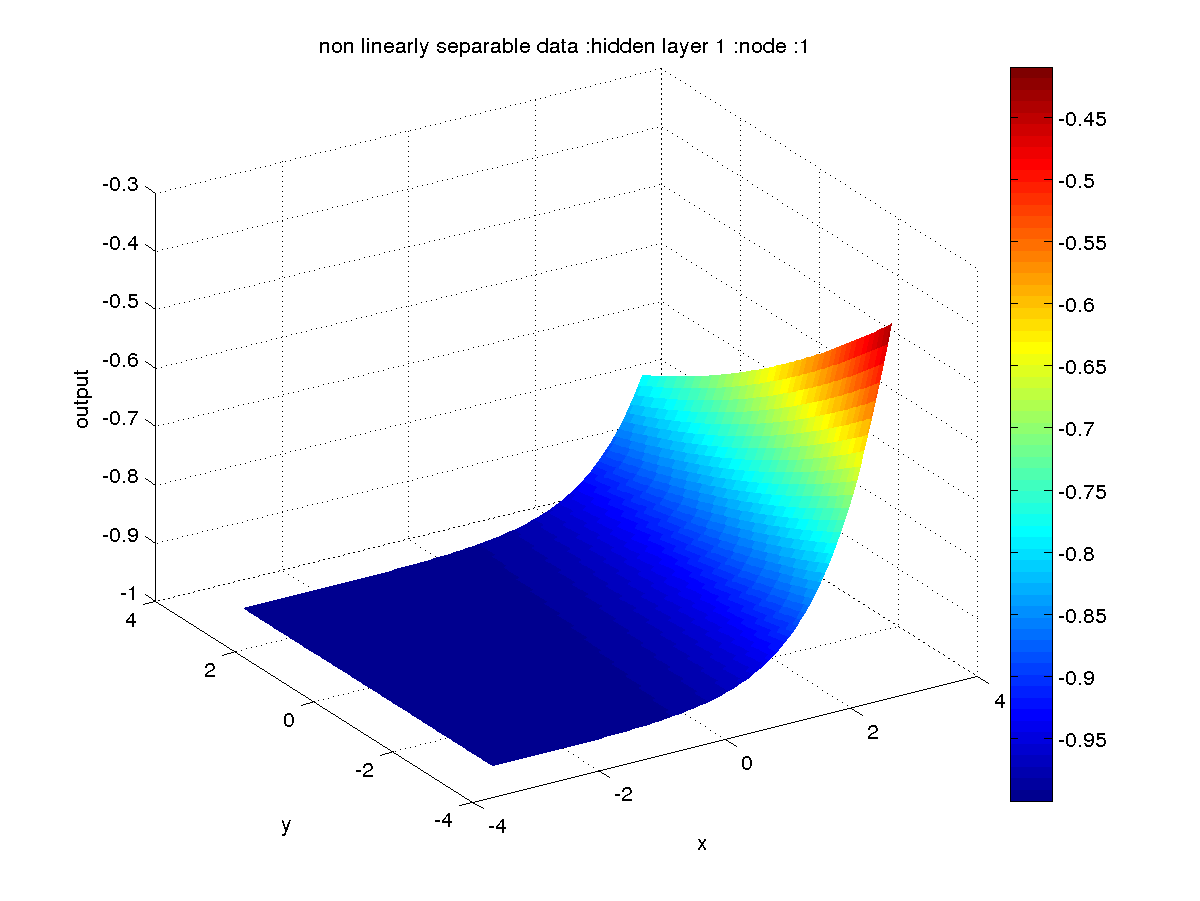
\includegraphics[scale=0.25]{./pics/nonlinearlyseparable/_4_2/_4_2_epoch_2_hidden layer 1 :1}  & 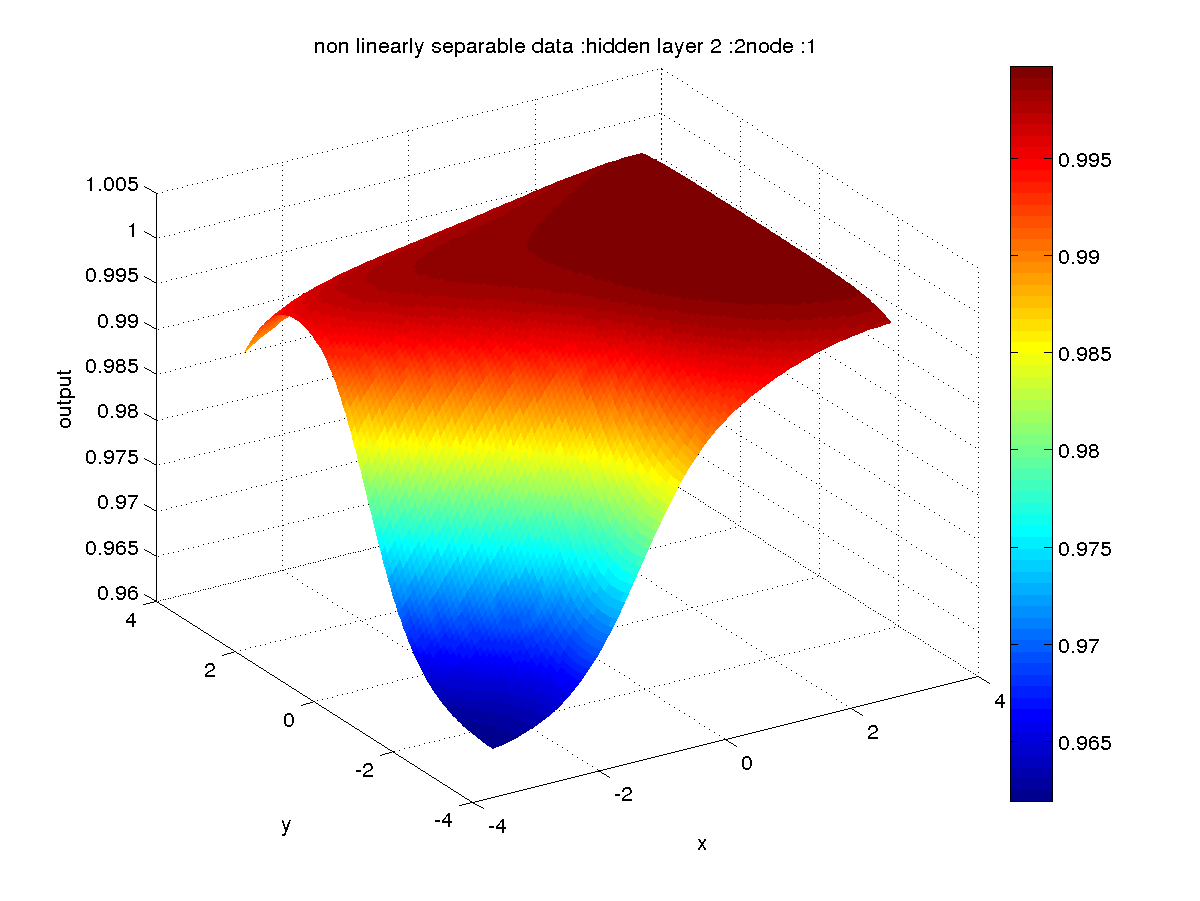
\includegraphics[scale=0.25]{./pics/nonlinearlyseparable/_4_2/_4_2_epoch_2_hidden layer 2 :21} & 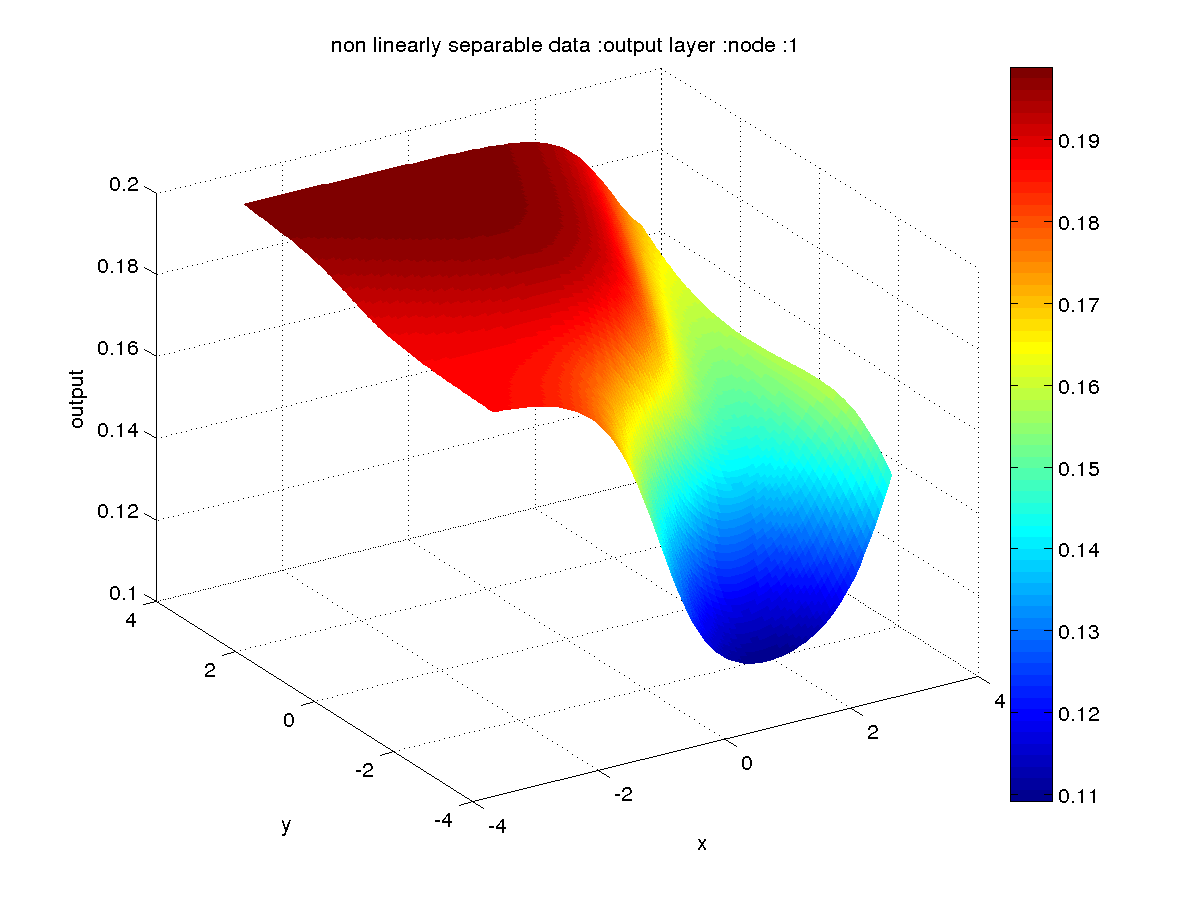
\includegraphics[scale=0.25]{./pics/nonlinearlyseparable/_4_2/_4_2_epoch_2_output layer :1}\\ 
    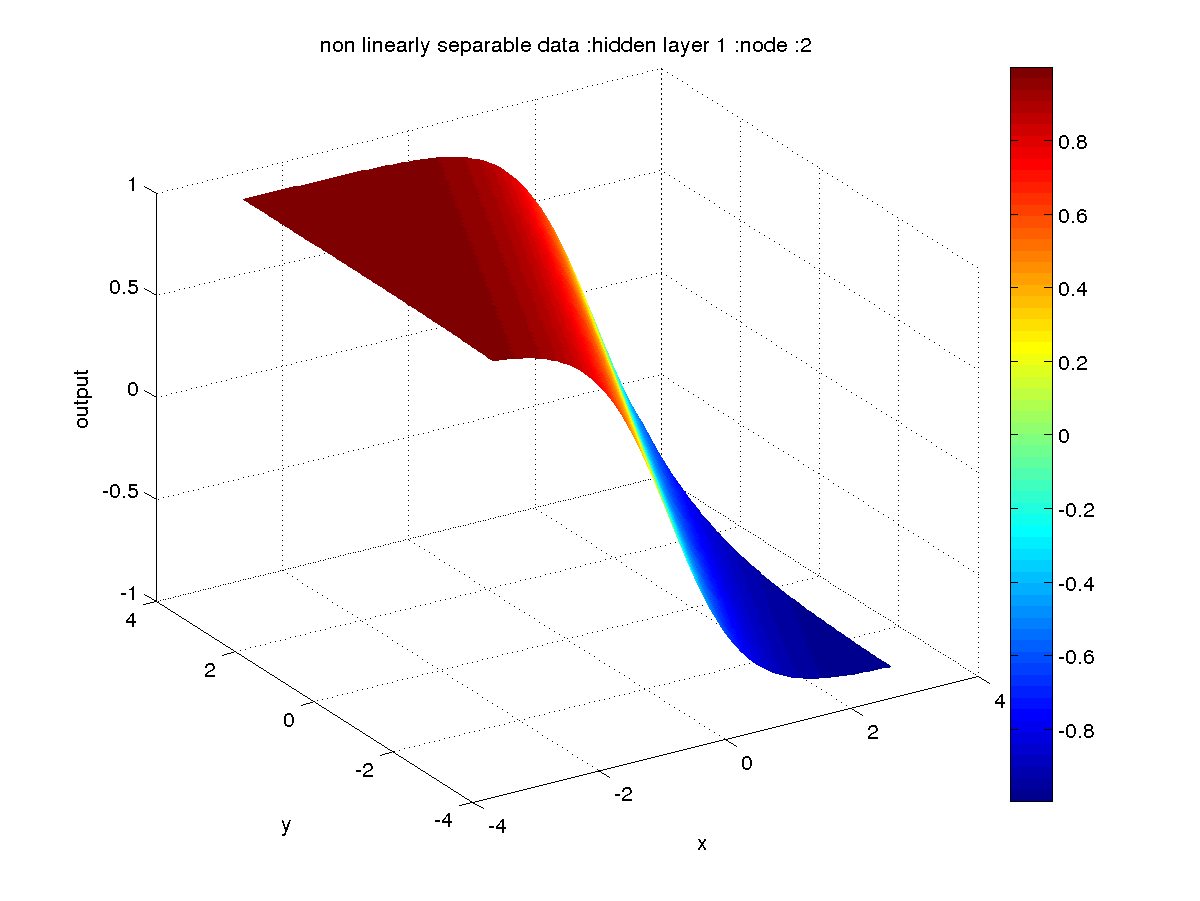
\includegraphics[scale=0.25]{./pics/nonlinearlyseparable/_4_2/_4_2_epoch_2_hidden layer 1 :2} &  & 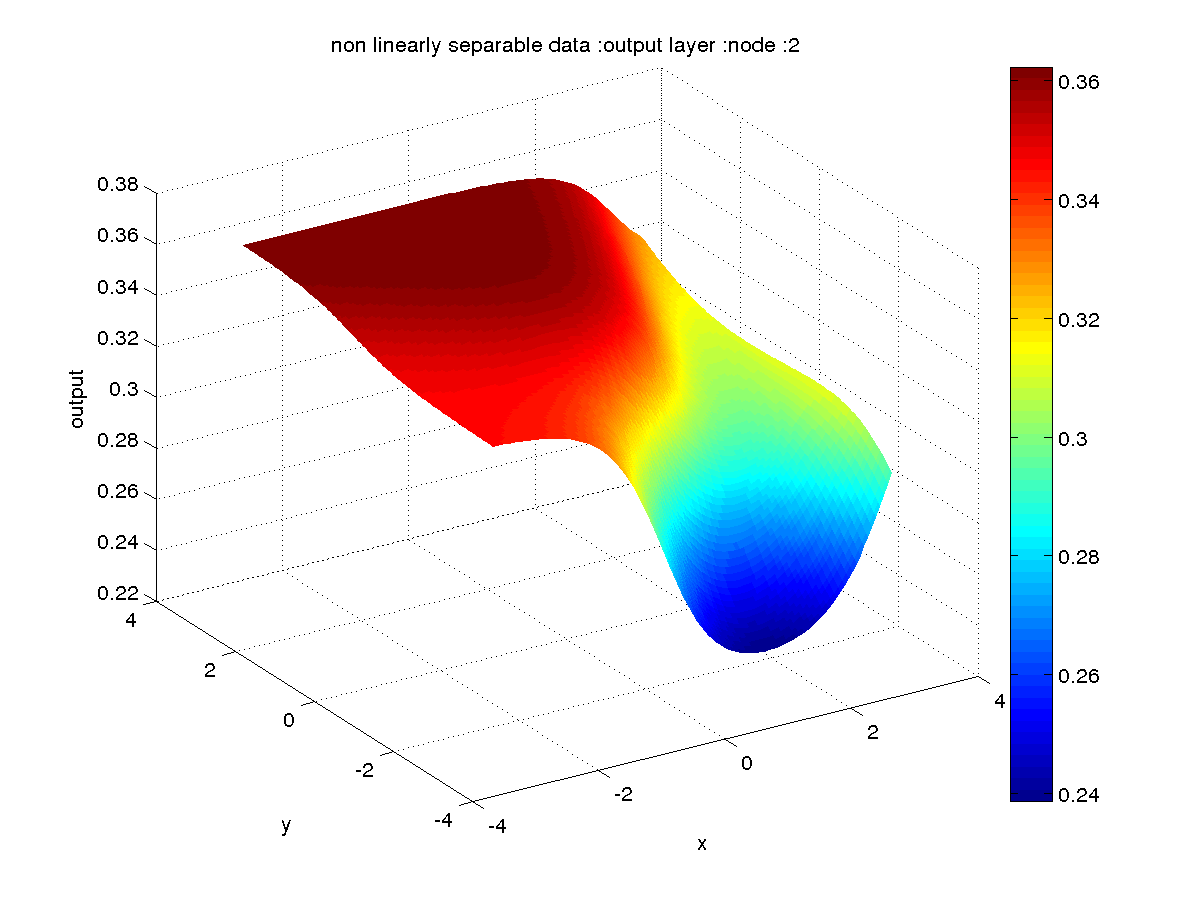
\includegraphics[scale=0.25]{./pics/nonlinearlyseparable/_4_2/_4_2_epoch_2_output layer :2} \\ 
    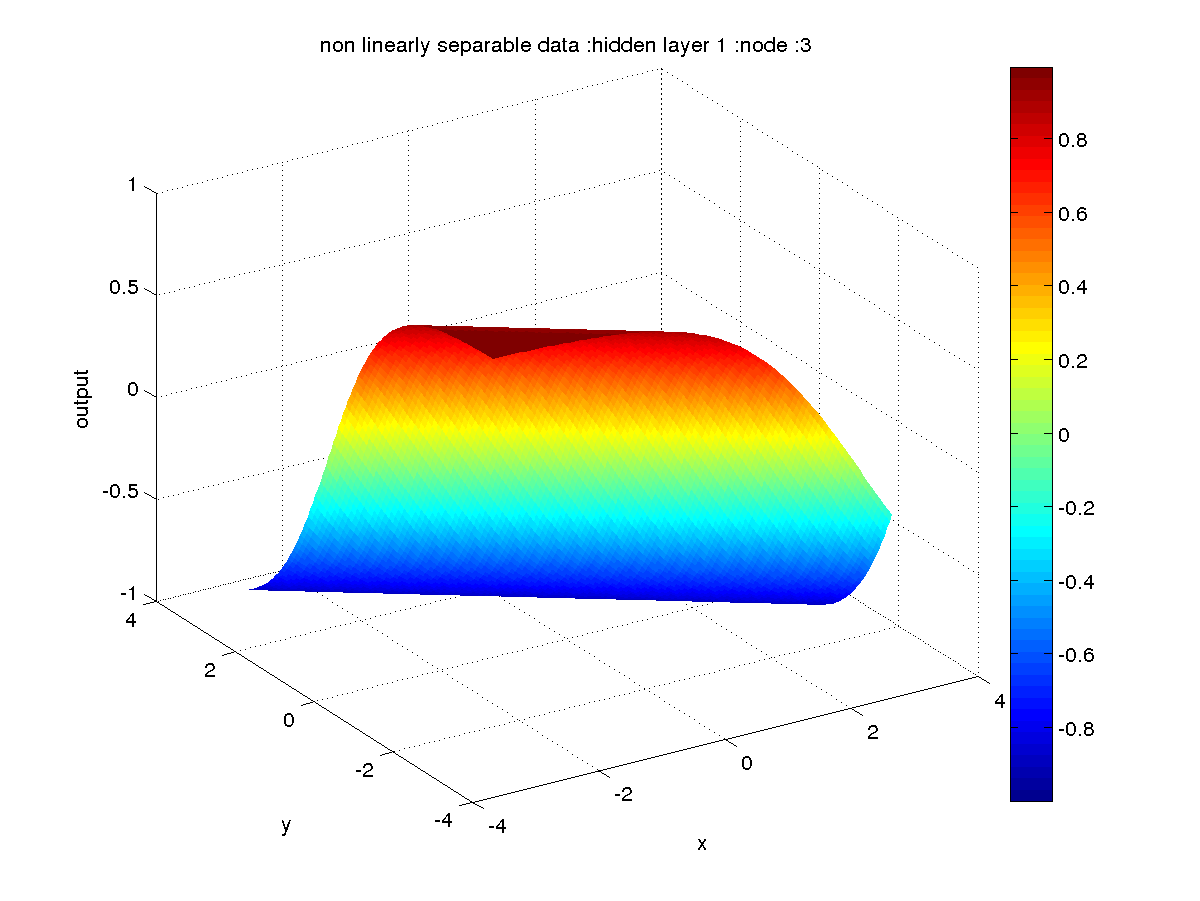
\includegraphics[scale=0.25]{./pics/nonlinearlyseparable/_4_2/_4_2_epoch_2_hidden layer 1 :3} & 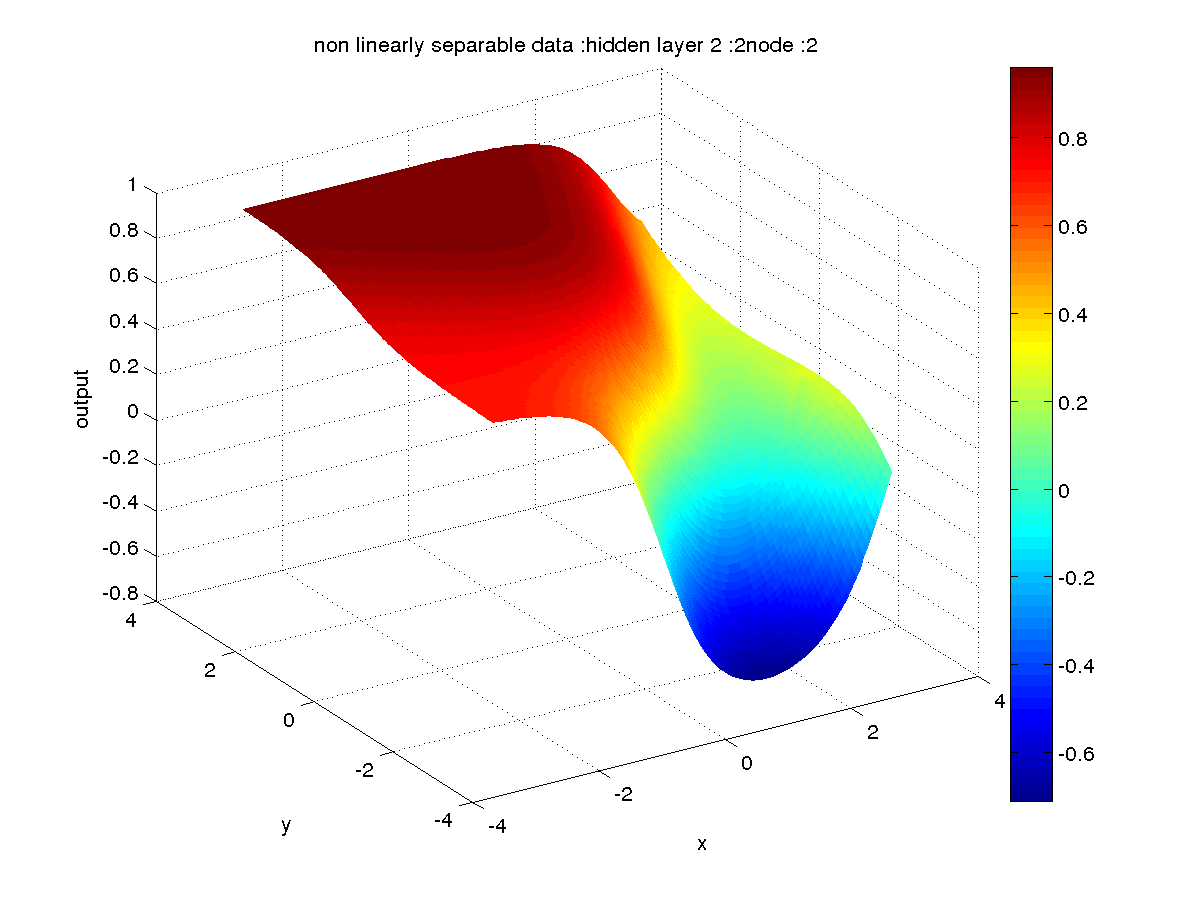
\includegraphics[scale=0.25]{./pics/nonlinearlyseparable/_4_2/_4_2_epoch_2_hidden layer 2 :22} & 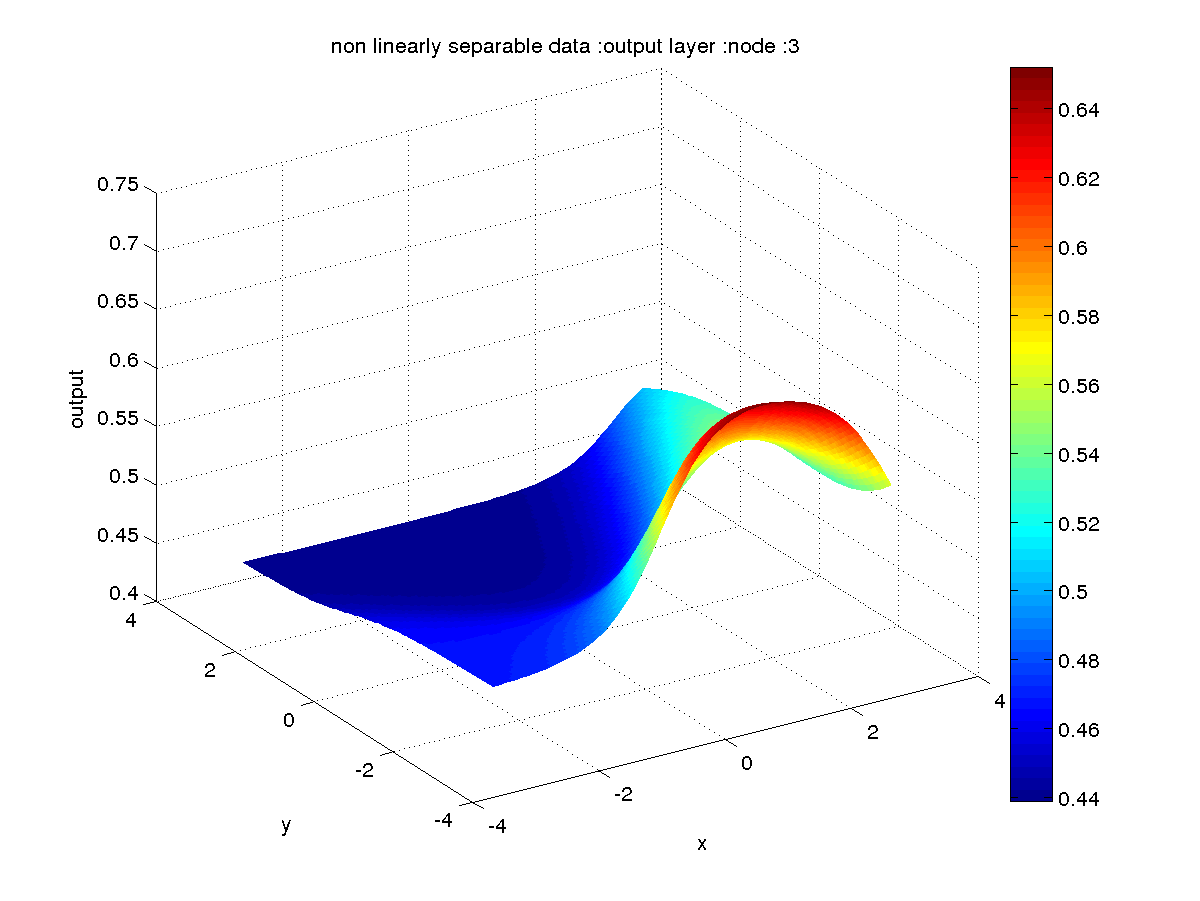
\includegraphics[scale=0.25]{./pics/nonlinearlyseparable/_4_2/_4_2_epoch_2_output layer :3}\\
    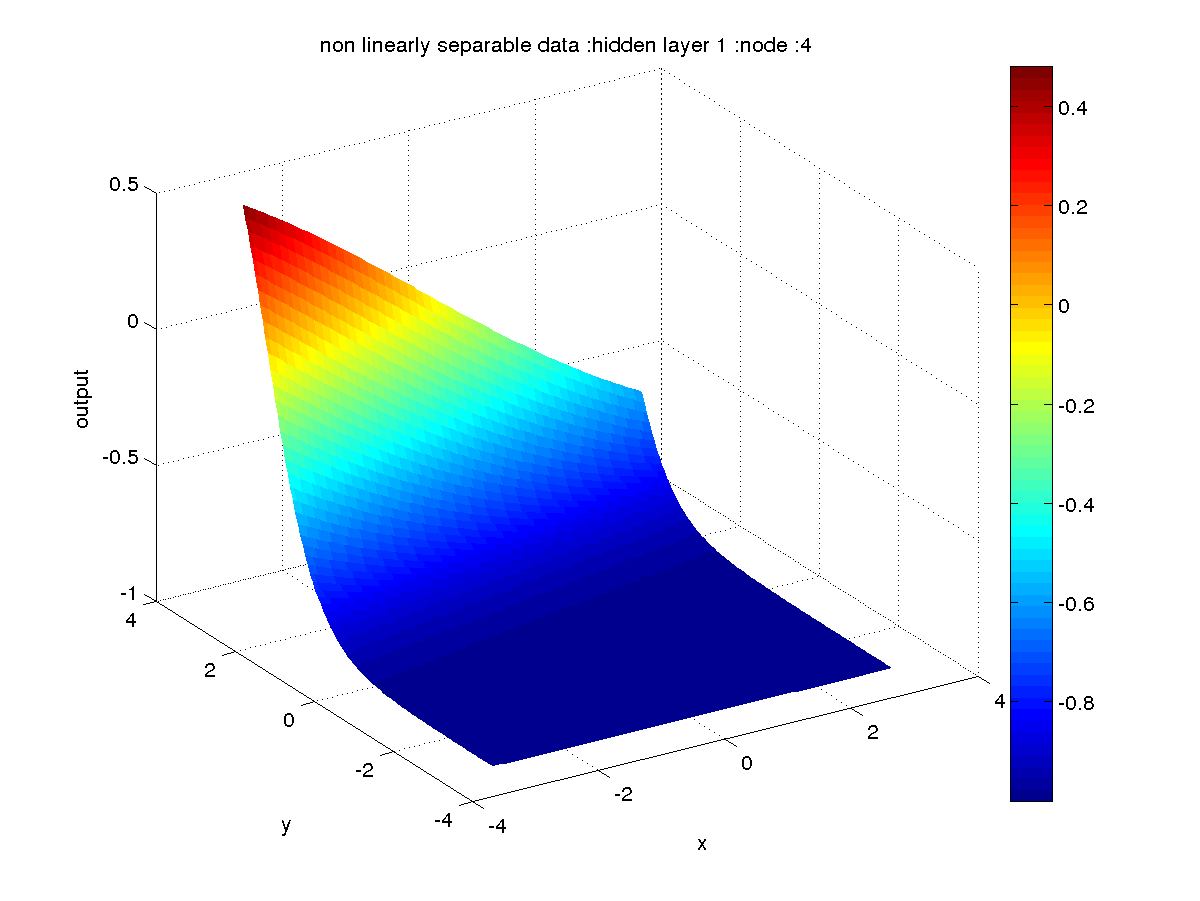
\includegraphics[scale=0.25]{./pics/nonlinearlyseparable/_4_2/_4_2_epoch_2_hidden layer 1 :4} &  & \\ 
    \hline
  \end{longtable}
\end{center}

\newpage
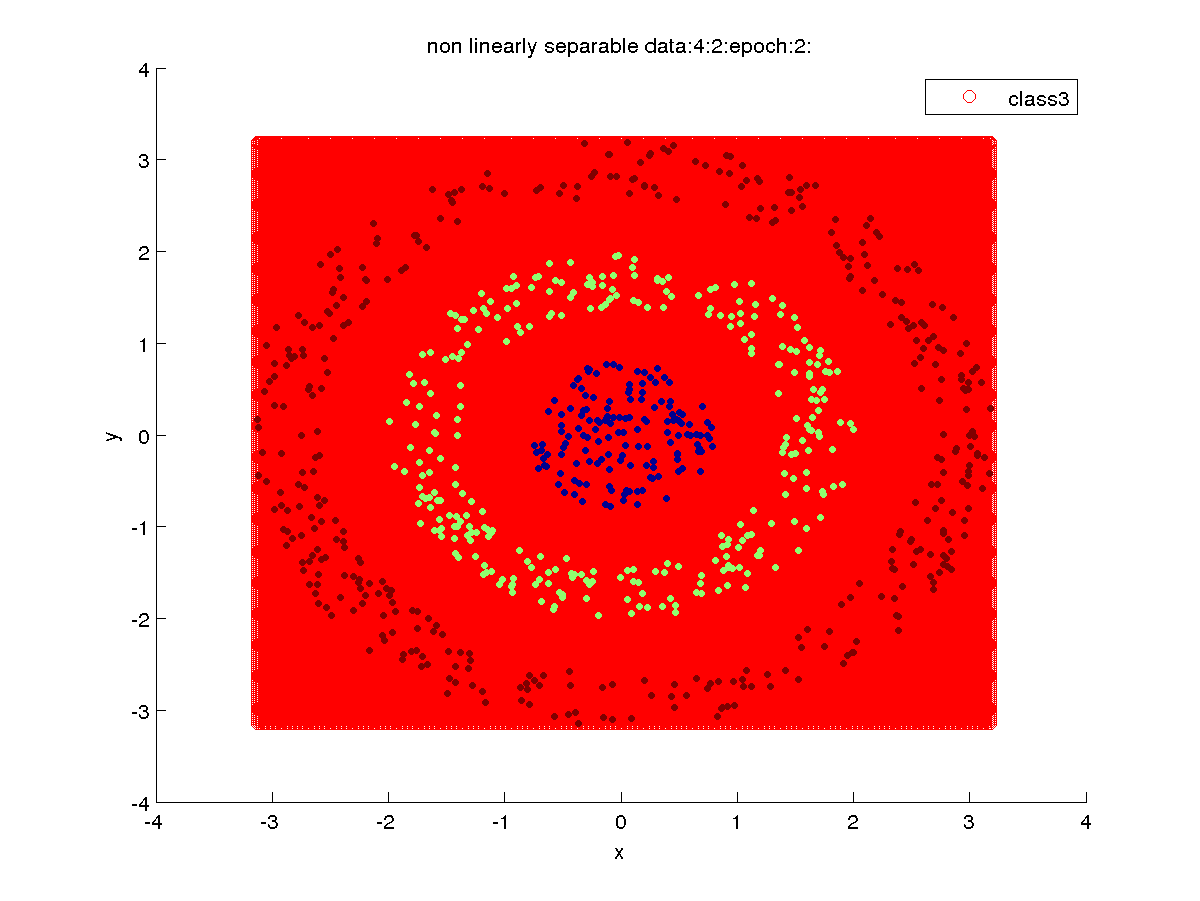
\includegraphics[scale=0.3]{./pics/nonlinearlyseparable/_4_2/_4_2_epoch_2_decisionBoundary}
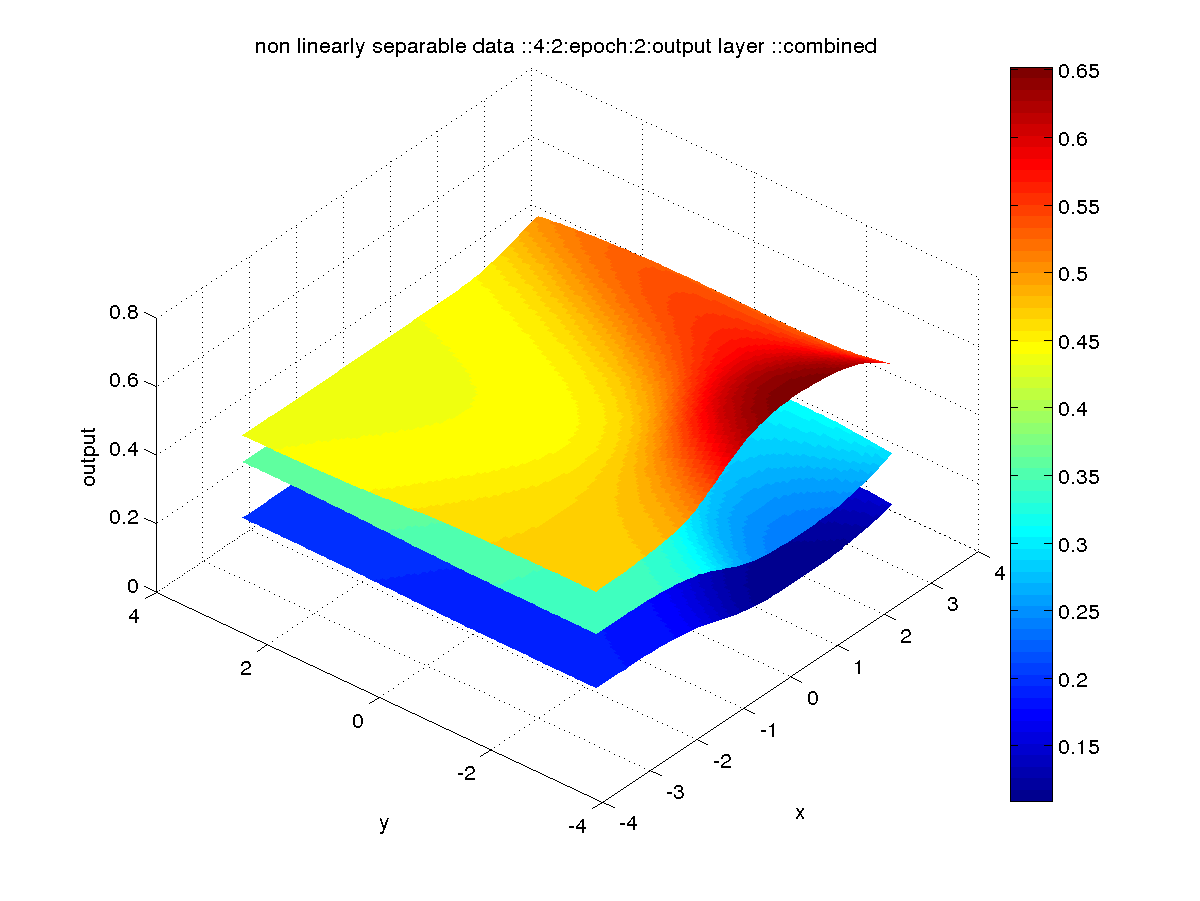
\includegraphics[scale=0.3]{./pics/nonlinearlyseparable/_4_2/_4_2_epoch_2_output layer :_combined}
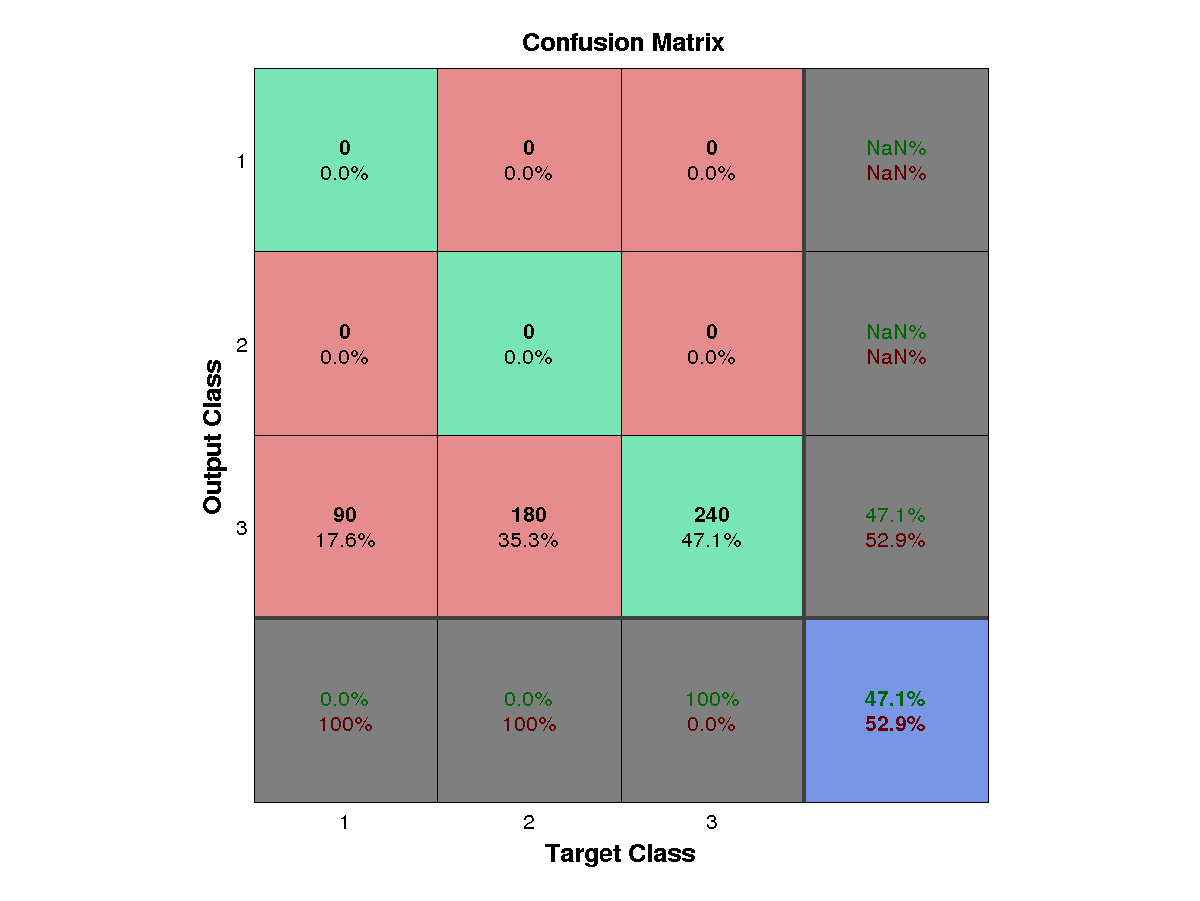
\includegraphics[scale=0.3]{./pics/nonlinearlyseparable/_4_2/_4_2_epoch_2_confusion}

\myparagraph{After 10 epochs}
\begin{center}
  \begin{longtable}{ c | c | r }
	\multicolumn{1}{c}{Hidden layer-1 } & 
	\multicolumn{1}{c}{Hidden layer-2 } & 
	\multicolumn{1}{c}{Output layer } \\
    \hline
    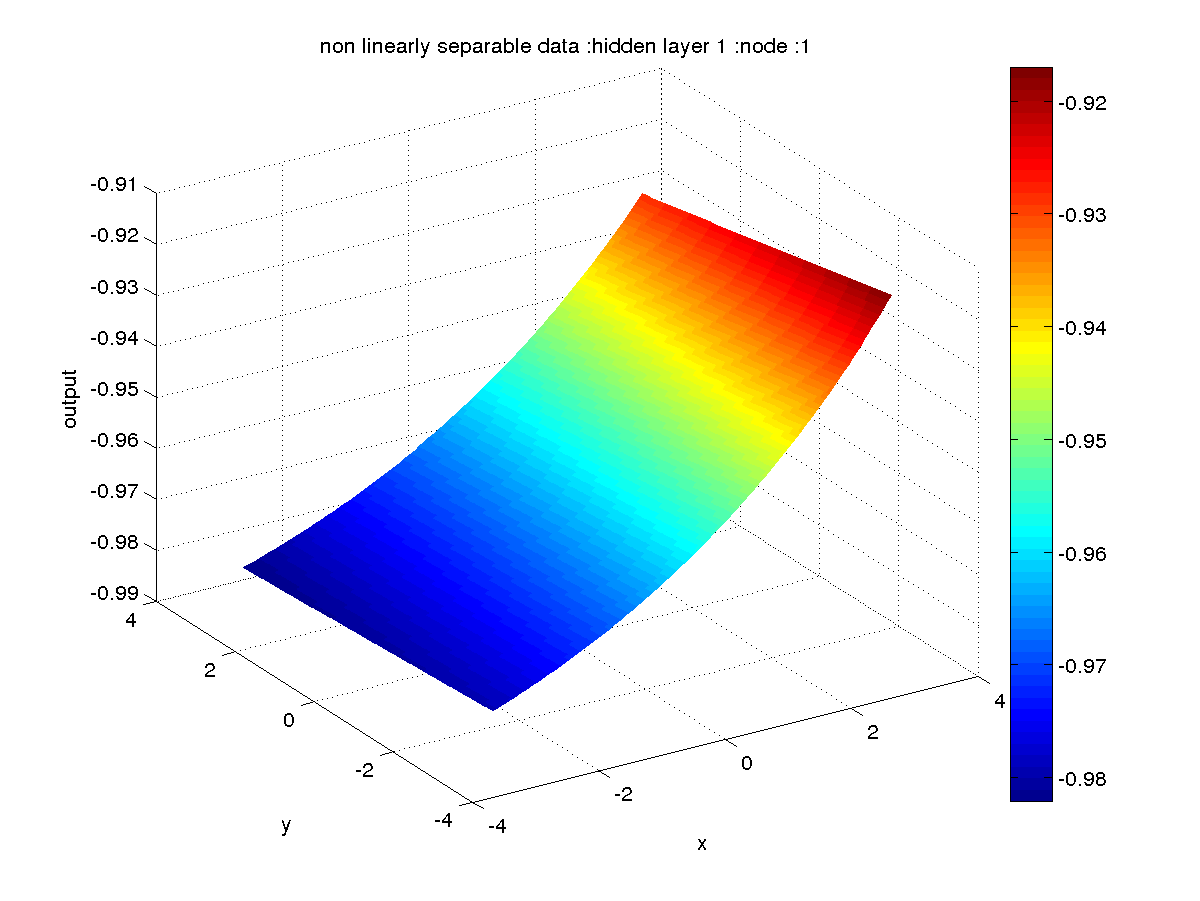
\includegraphics[scale=0.25]{./pics/nonlinearlyseparable/_4_2/_4_2_epoch_10_hidden layer 1 :1}  & 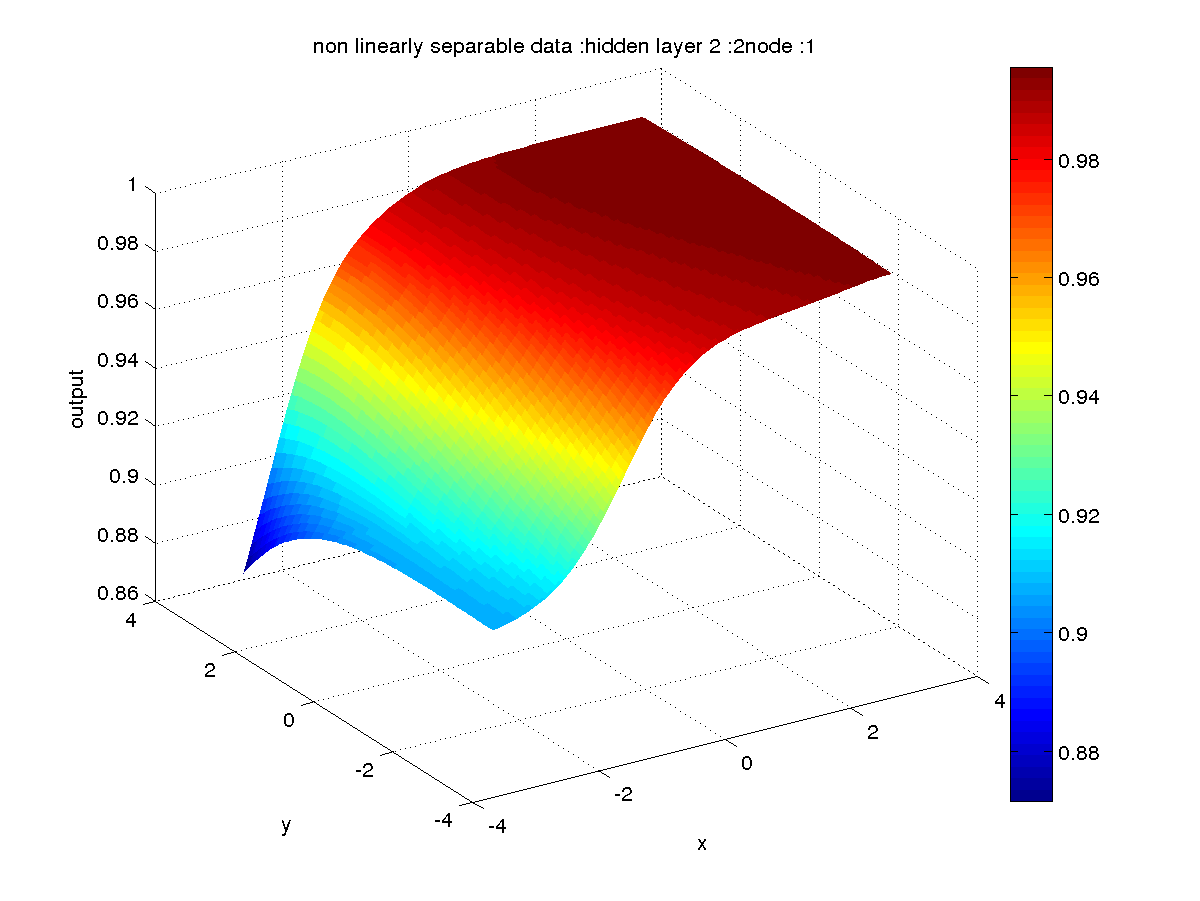
\includegraphics[scale=0.25]{./pics/nonlinearlyseparable/_4_2/_4_2_epoch_10_hidden layer 2 :21} & 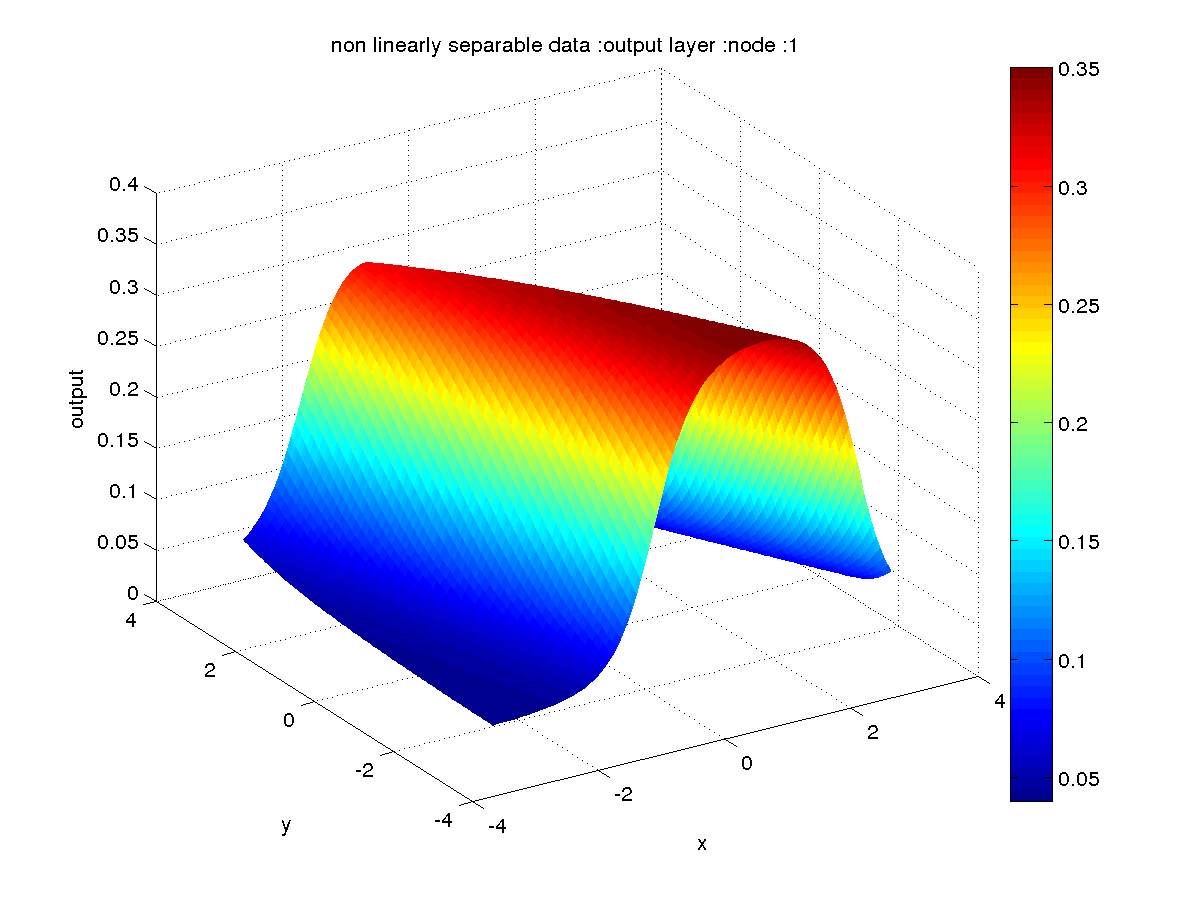
\includegraphics[scale=0.25]{./pics/nonlinearlyseparable/_4_2/_4_2_epoch_10_output layer :1}\\ 
    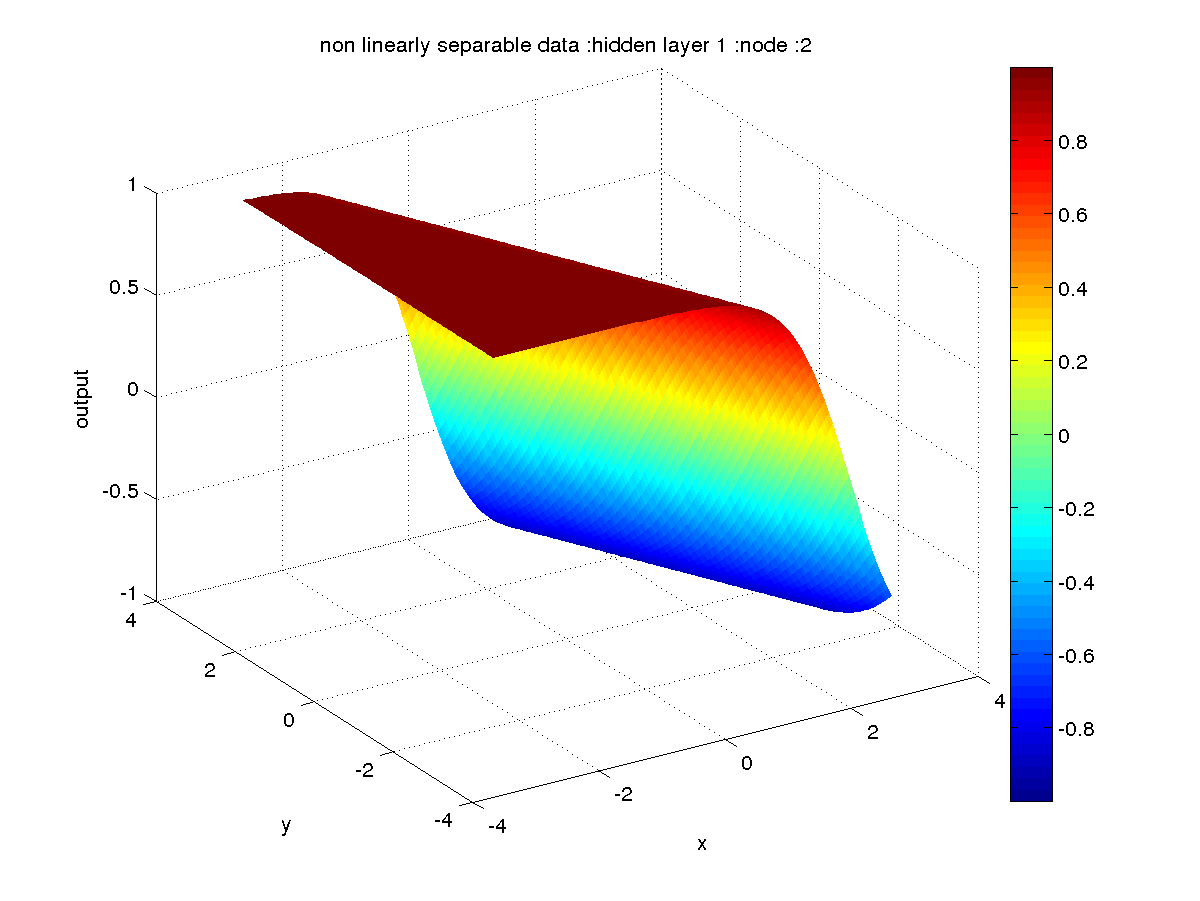
\includegraphics[scale=0.25]{./pics/nonlinearlyseparable/_4_2/_4_2_epoch_10_hidden layer 1 :2} &  & 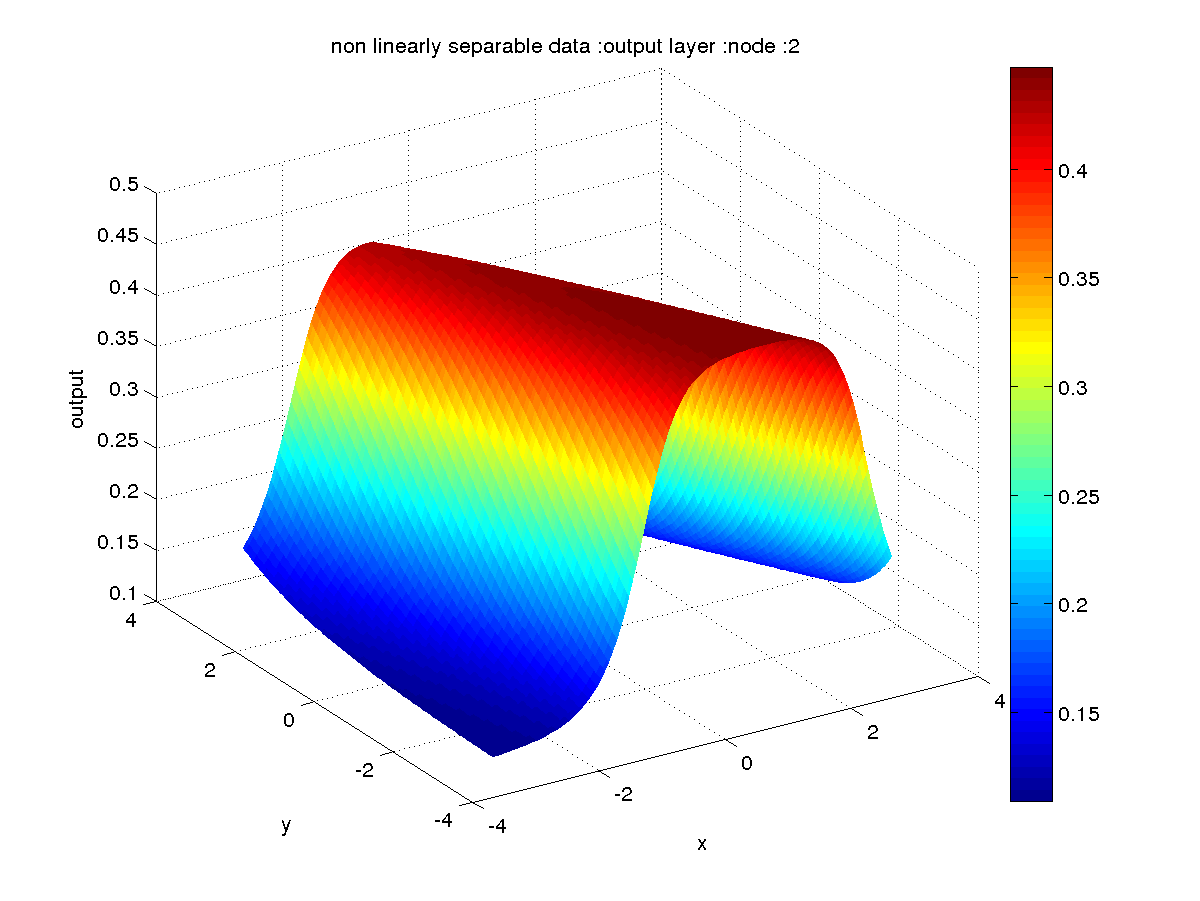
\includegraphics[scale=0.25]{./pics/nonlinearlyseparable/_4_2/_4_2_epoch_10_output layer :2} \\ 
    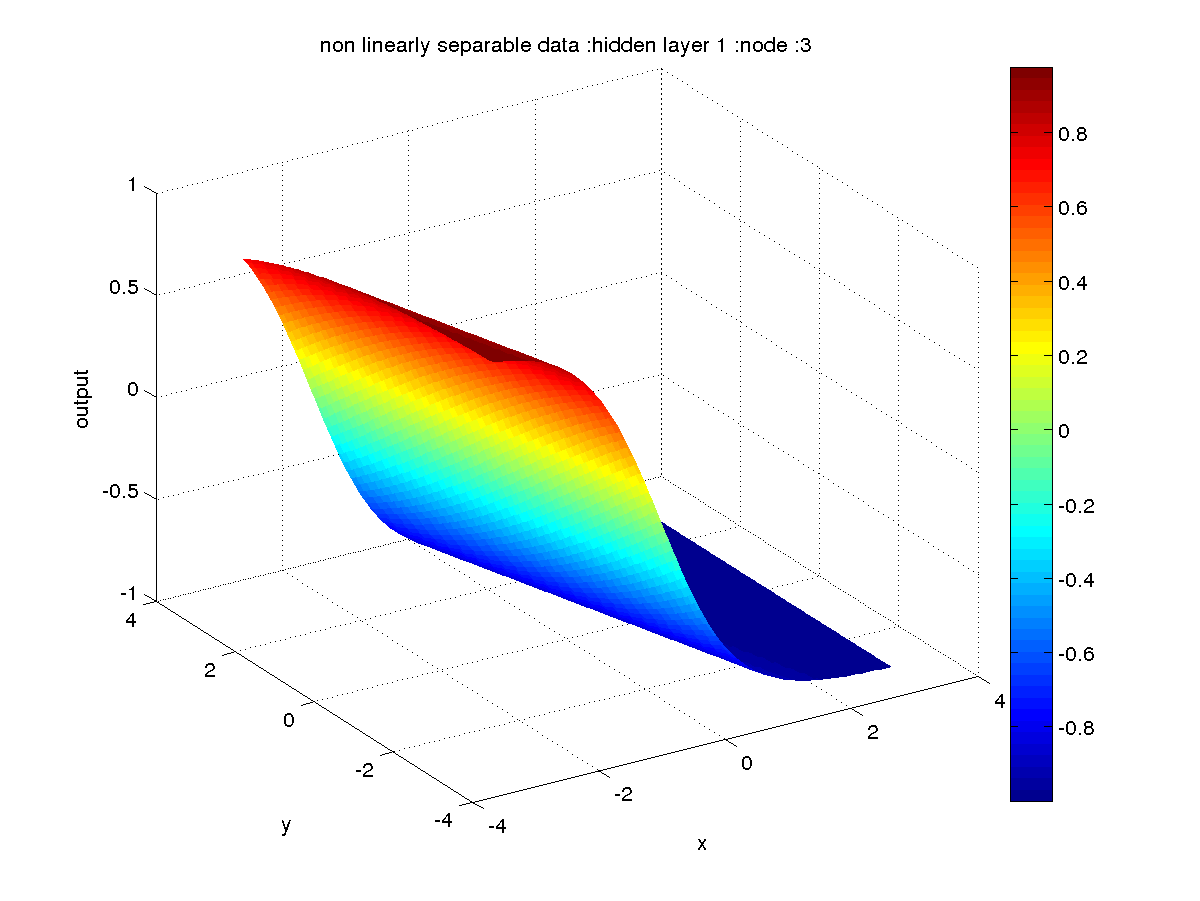
\includegraphics[scale=0.25]{./pics/nonlinearlyseparable/_4_2/_4_2_epoch_10_hidden layer 1 :3} & \includegraphics[scale=0.25]{./pics/nonlinearlyseparable/_4_2/_4_2_epoch_10_hidden layer 2 :22} & \includegraphics[scale=0.25]{./pics/nonlinearlyseparable/_4_2/_4_2_epoch_10_output layer :3}\\
    \includegraphics[scale=0.25]{./pics/nonlinearlyseparable/_4_2/_4_2_epoch_10_hidden layer 1 :4} &  & \\ 
    \hline
  \end{longtable}
\end{center}

\includegraphics[scale=0.3]{./pics/nonlinearlyseparable/_4_2/_4_2_epoch_10_decisionBoundary}
\includegraphics[scale=0.3]{./pics/nonlinearlyseparable/_4_2/_4_2_epoch_10_output layer :_combined}
\includegraphics[scale=0.3]{./pics/nonlinearlyseparable/_4_2/_4_2_epoch_10_confusion}

\newpage
\myparagraph{After 50 epochs}
\begin{center}
  \begin{longtable}{ c | c | r }
	\multicolumn{1}{c}{Hidden layer-1 } & 
	\multicolumn{1}{c}{Hidden layer-2 } & 
	\multicolumn{1}{c}{Output layer } \\
    \hline
    \includegraphics[scale=0.25]{./pics/nonlinearlyseparable/_4_2/_4_2_epoch_50_hidden layer 1 :1}  & \includegraphics[scale=0.25]{./pics/nonlinearlyseparable/_4_2/_4_2_epoch_50_hidden layer 2 :21} & \includegraphics[scale=0.25]{./pics/nonlinearlyseparable/_4_2/_4_2_epoch_50_output layer :1}\\ 
    \includegraphics[scale=0.25]{./pics/nonlinearlyseparable/_4_2/_4_2_epoch_50_hidden layer 1 :2} &  & \includegraphics[scale=0.25]{./pics/nonlinearlyseparable/_4_2/_4_2_epoch_50_output layer :2} \\ 
    \includegraphics[scale=0.25]{./pics/nonlinearlyseparable/_4_2/_4_2_epoch_50_hidden layer 1 :3} & \includegraphics[scale=0.25]{./pics/nonlinearlyseparable/_4_2/_4_2_epoch_50_hidden layer 2 :22} & \includegraphics[scale=0.25]{./pics/nonlinearlyseparable/_4_2/_4_2_epoch_50_output layer :3}\\
    \includegraphics[scale=0.25]{./pics/nonlinearlyseparable/_4_2/_4_2_epoch_50_hidden layer 1 :4} &  & \\ 
    \hline
  \end{longtable}
\end{center}

\includegraphics[scale=0.3]{./pics/nonlinearlyseparable/_4_2/_4_2_epoch_50_decisionBoundary}
\includegraphics[scale=0.3]{./pics/nonlinearlyseparable/_4_2/_4_2_epoch_50_output layer :_combined}
\includegraphics[scale=0.3]{./pics/nonlinearlyseparable/_4_2/_4_2_epoch_50_confusion}

\newpage
\myparagraph{After 100 epochs}
\begin{center}
  \begin{longtable}{ c | c | r  }
	\multicolumn{1}{c}{Hidden layer-1 } & 
	\multicolumn{1}{c}{Hidden layer-2 } & 
	\multicolumn{1}{c}{Output layer } \\
    \hline
    \includegraphics[scale=0.25]{./pics/nonlinearlyseparable/_4_2/_4_2_epoch_100_hidden layer 1 :1}  & \includegraphics[scale=0.25]{./pics/nonlinearlyseparable/_4_2/_4_2_epoch_100_hidden layer 2 :21} & \includegraphics[scale=0.25]{./pics/nonlinearlyseparable/_4_2/_4_2_epoch_100_output layer :1}\\ 
    \includegraphics[scale=0.25]{./pics/nonlinearlyseparable/_4_2/_4_2_epoch_100_hidden layer 1 :2} &  & \includegraphics[scale=0.25]{./pics/nonlinearlyseparable/_4_2/_4_2_epoch_100_output layer :2} \\ 
    \includegraphics[scale=0.25]{./pics/nonlinearlyseparable/_4_2/_4_2_epoch_100_hidden layer 1 :3} & \includegraphics[scale=0.25]{./pics/nonlinearlyseparable/_4_2/_4_2_epoch_100_hidden layer 2 :22} & \includegraphics[scale=0.25]{./pics/nonlinearlyseparable/_4_2/_4_2_epoch_100_output layer :3}\\
    \includegraphics[scale=0.25]{./pics/nonlinearlyseparable/_4_2/_4_2_epoch_100_hidden layer 1 :4} &  & \\ 
    \hline
  \end{longtable}
\end{center}

\includegraphics[scale=0.3]{./pics/nonlinearlyseparable/_4_2/_4_2_epoch_100_decisionBoundary}
\includegraphics[scale=0.3]{./pics/nonlinearlyseparable/_4_2/_4_2_epoch_100_output layer :_combined}
\includegraphics[scale=0.3]{./pics/nonlinearlyseparable/_4_2/_4_2_epoch_100_confusion}

\newpage
\myparagraph{After training}
\begin{center}
  \begin{longtable}{ c | c | r }
	\multicolumn{1}{c}{Hidden layer-1 } & 
	\multicolumn{1}{c}{Hidden layer-2 } & 
	\multicolumn{1}{c}{Output layer } \\
    \hline
    \includegraphics[scale=0.25]{./pics/nonlinearlyseparable/_4_2/_4_2_epoch_Inf_hidden layer 1 :1}  & \includegraphics[scale=0.25]{./pics/nonlinearlyseparable/_4_2/_4_2_epoch_Inf_hidden layer 2 :21} & \includegraphics[scale=0.25]{./pics/nonlinearlyseparable/_4_2/_4_2_epoch_Inf_output layer :1}\\ 
    \includegraphics[scale=0.25]{./pics/nonlinearlyseparable/_4_2/_4_2_epoch_Inf_hidden layer 1 :2} &  & \includegraphics[scale=0.25]{./pics/nonlinearlyseparable/_4_2/_4_2_epoch_Inf_output layer :2} \\ 
    \includegraphics[scale=0.25]{./pics/nonlinearlyseparable/_4_2/_4_2_epoch_Inf_hidden layer 1 :3} & \includegraphics[scale=0.25]{./pics/nonlinearlyseparable/_4_2/_4_2_epoch_Inf_hidden layer 2 :22} & \includegraphics[scale=0.25]{./pics/nonlinearlyseparable/_4_2/_4_2_epoch_Inf_output layer :3}\\
    \includegraphics[scale=0.25]{./pics/nonlinearlyseparable/_4_2/_4_2_epoch_Inf_hidden layer 1 :4} &  & \\ 
    \hline
  \end{longtable}
\end{center}

\includegraphics[scale=0.3]{./pics/nonlinearlyseparable/_4_2/_4_2_epoch_Inf_decisionBoundary}
\includegraphics[scale=0.3]{./pics/nonlinearlyseparable/_4_2/_4_2_epoch_Inf_output layer :_combined}
\includegraphics[scale=0.3]{./pics/nonlinearlyseparable/_4_2/_4_2_epoch_Inf_confusion}

\newpage
\begin{figure}[!ht]
\begin{subfigure}{.5\textwidth}
\caption{confusion matrix \\ of train data}
\includegraphics[scale=0.5]{./pics/nonlinearlyseparable/_4_2/_4_2_epoch_Inf_confusiontrain}
\end{subfigure}
\begin{subfigure}{.5\textwidth}
\caption{confusion matrix \\ of test data}
\includegraphics[scale=0.5]{./pics/nonlinearlyseparable/_4_2/_4_2_epoch_Inf_confusiontest}
\end{subfigure}
\end{figure}

\myparagraph{Observations}

\begin{itemize}
  \item Except the model complexity with hidden-layer1 count = 2, all other models are giving miss-percentage of 0\%.
  \item During initial epochs (epochs 1, 2) of training, the model is in arbitrary state and it is predicting all the examples as class-3. After the training runs for multiple epochs, at 10th epoch, we can notice that the model is learning about the other classes (class-2).
  \item At $50^{th}$ epoch, the model has almost learned the boundary of different classes and trying to stabilize the boundaries. Still, we can see that the probabilities of appropriate classes are not high enough, which reveals that the model is not so confident about the class boundaries yet.
  \item At $100^{th}$ iteration, we can notice from the combined plot of output layer nodes, that the confidence of model has been increased and boundaries are almost freezed to give better efficiency.
\end{itemize}

\newpage
\subsection{Overlapping data}

The dataset contains 4 classes which are overlapped as shown in figure below. 
The dataset contains 500 points (train = 250, validation = 150, test = 100) in each of the 4 classes.

\begin{figure}[!ht]
\begin{subfigure}{.5\textwidth}
  \caption{Plot of the data}
\includegraphics[scale=0.4]{pics/overlapping_data/dataPlot}
\end{subfigure}
\begin{subfigure}{.5\textwidth}
  \caption{Validation Miss percentage based\\ on model complextites}
\includegraphics[scale=0.2]{pics/overlapping_data/overlapping data_validationerror}
\end{subfigure}
\end{figure}


Based on the validation data miss percentage plot, the model of (hiddenlayer1 \#nodes = 14, hiddenlayer2 \#nodes = 16) is chosen as the best model.

\subsubsection{MLFFNN with 2 Hidden layers}

\myparagraph{Decision boundary \& Confusion matrix}

\includegraphics[scale=0.3]{./pics/overlapping_data/_14_16/_14_16_epoch_Inf_decisionBoundary}
\includegraphics[scale=0.3]{./pics/overlapping_data/_14_16/_14_16_epoch_Inf_output layer :_combined}
\includegraphics[scale=0.3]{./pics/overlapping_data/_14_16/_14_16_epoch_Inf_confusion}

\begin{figure}[!ht]
\begin{subfigure}{.5\textwidth}
\caption{confusion matrix \\ of train data}
\includegraphics[scale=0.4]{./pics/overlapping_data/_14_16/_14_16_epoch_Inf_confusiontrain}
\end{subfigure}
\begin{subfigure}{.5\textwidth}
\caption{confusion matrix \\ of test data}
\includegraphics[scale=0.5]{./pics/overlapping_data/_14_16/_14_16_epoch_Inf_confusiontest}
\end{subfigure}
\end{figure}

\myparagraph{Observations}

\begin{itemize}
  \item Since, the data is overlapped, the network needs more hidden nodes to model the data. The best model (hiddenlayer1 \#nodes = 14, hiddenlayer2 \#nodes = 16) converges in \~80 epochs. 
  \item The decision boundary learned by Neural network is complex non-linear function.
  \item Adding further nodes does not seem to increase the accuracy, as we see from the miss percentage plot.
\end{itemize}

\clearpage
\newpage
\section{Regression}
\subsection{MLFFNN}

\subsubsection{MLFFNN with 1 Hidden layer (100 points from system with less intrinsic noise)}

It is interesting to see that even with 100 points, the MLFFNN model with single hidden layer (of 6 nodes) is able to \\
generalize well for the univariate data. The model is selected based on the MSE (Mean Squared Error) criteria.


\begin{figure}[!ht]
\begin{subfigure}{.5\textwidth}
  \caption{Training data plot}
\includegraphics[scale=0.5]{pics/univariate100/dataPlot}
\end{subfigure}
\begin{subfigure}{.5\textwidth}
\caption{Validation performance (Mean squared Error)}
\includegraphics[scale=0.2]{pics/univariate100/univariate continuous data (100 points)_validationerror}
\end{subfigure}
\end{figure}

\newpage
\myparagraph{Scatter plot with model output and target output of model with HiddenLayer1 nodes = 6}

\includegraphics[scale=0.4]{./pics/univariate100/_6/_6_epoch_Inf_train-data_scatter3d}
\includegraphics[scale=0.4]{./pics/univariate100/_6/_6_epoch_Inf_train-data_scatter2d}
\includegraphics[scale=0.4]{./pics/univariate100/_6/_6_epoch_Inf_validation-data_scatter3d}
\includegraphics[scale=0.4]{./pics/univariate100/_6/_6_epoch_Inf_validation-data_scatter2d}
\includegraphics[scale=0.4]{./pics/univariate100/_6/_6_epoch_Inf_test-data_scatter3d}
\includegraphics[scale=0.4]{./pics/univariate100/_6/_6_epoch_Inf_test-data_scatter2d}


\subsubsection{MLFFNN with 1 Hidden layer (2000 points from system with less intrinsic noise)}

With 2000 points, the MLFFNN model with \textbf{single hidden layer (of 11 nodes)} given better validation performance.


\begin{figure}[!ht]
\begin{subfigure}{.5\textwidth}
  \caption{Training data plot}
\includegraphics[scale=0.5]{pics/univariate/dataPlot}
\end{subfigure}
\begin{subfigure}{.5\textwidth}
\caption{Validation performance (Mean squared Error)}
\includegraphics[scale=0.2]{pics/univariate/univariate continuous data_validationerror}
\end{subfigure}
\end{figure}

\newpage
\myparagraph{Scatter plot with model output and target output of model with HiddenLayer1 nodes = 11}

\includegraphics[scale=0.4]{./pics/univariate/_11/_11_epoch_Inf_train-data_scatter3d}
\includegraphics[scale=0.4]{./pics/univariate/_11/_11_epoch_Inf_train-data_scatter2d}
\includegraphics[scale=0.4]{./pics/univariate/_11/_11_epoch_Inf_validation-data_scatter3d}
\includegraphics[scale=0.4]{./pics/univariate/_11/_11_epoch_Inf_validation-data_scatter2d}
\includegraphics[scale=0.4]{./pics/univariate/_11/_11_epoch_Inf_test-data_scatter3d}
\includegraphics[scale=0.4]{./pics/univariate/_11/_11_epoch_Inf_test-data_scatter2d}


\subsubsection{MLFFNN with 1 Hidden layer (100 points from system with more intrinsic noise)}

It is interesting to see that even with 100 points, the MLFFNN model with single hidden layer (of 6 nodes) is able to \\
generalize well for the univariate data. The model is selected based on the MSE (Mean Squared Error) criteria.


\begin{figure}[!ht]
\begin{subfigure}{.5\textwidth}
  \caption{Training data plot}
\includegraphics[scale=0.5]{pics/univariate100_morenoise/dataPlot}
\end{subfigure}
\begin{subfigure}{.5\textwidth}
\caption{Validation performance (Mean squared Error)}
\includegraphics[scale=0.2]{pics/univariate100_morenoise/univariate continuous data (100 points)_validationerror}
\end{subfigure}
\end{figure}

\newpage
\myparagraph{Scatter plot with model output and target output of model with HiddenLayer1 nodes = 6}

\includegraphics[scale=0.4]{./pics/univariate100_morenoise/_6/_6_epoch_Inf_train-data_scatter3d}
\includegraphics[scale=0.4]{./pics/univariate100_morenoise/_6/_6_epoch_Inf_train-data_scatter2d}
\includegraphics[scale=0.4]{./pics/univariate100_morenoise/_6/_6_epoch_Inf_validation-data_scatter3d}
\includegraphics[scale=0.4]{./pics/univariate100_morenoise/_6/_6_epoch_Inf_validation-data_scatter2d}
\includegraphics[scale=0.4]{./pics/univariate100_morenoise/_6/_6_epoch_Inf_test-data_scatter3d}
\includegraphics[scale=0.4]{./pics/univariate100_morenoise/_6/_6_epoch_Inf_test-data_scatter2d}


\subsubsection{MLFFNN with 1 Hidden layer (2000 points from system with more intrinsic noise)}

With 2000 points, the MLFFNN model with \textbf{single hidden layer (of 3 nodes)} given better validation performance.


\begin{figure}[!ht]
\begin{subfigure}{.5\textwidth}
  \caption{Training data plot}
\includegraphics[scale=0.5]{pics/univariate_morenoise/dataPlot}
\end{subfigure}
\begin{subfigure}{.5\textwidth}
\caption{Validation performance (Mean squared Error)}
\includegraphics[scale=0.2]{pics/univariate_morenoise/univariate continuous data_validationerror}
\end{subfigure}
\end{figure}

\newpage
\myparagraph{Scatter plot with model output and target output of model with HiddenLayer1 nodes = 3}

\includegraphics[scale=0.4]{./pics/univariate_morenoise/_3/_3_epoch_Inf_train-data_scatter3d}
\includegraphics[scale=0.4]{./pics/univariate_morenoise/_3/_3_epoch_Inf_train-data_scatter2d}
\includegraphics[scale=0.4]{./pics/univariate_morenoise/_3/_3_epoch_Inf_validation-data_scatter3d}
\includegraphics[scale=0.4]{./pics/univariate_morenoise/_3/_3_epoch_Inf_validation-data_scatter2d}
\includegraphics[scale=0.4]{./pics/univariate_morenoise/_3/_3_epoch_Inf_test-data_scatter3d}
\includegraphics[scale=0.4]{./pics/univariate_morenoise/_3/_3_epoch_Inf_test-data_scatter2d}

\newpage
\myparagraph{Scatter plot with model output and target output of model with HiddenLayer1 nodes = 8}

\includegraphics[scale=0.4]{./pics/univariate_morenoise/_8/_8_epoch_Inf_train-data_scatter3d}
\includegraphics[scale=0.4]{./pics/univariate_morenoise/_8/_8_epoch_Inf_train-data_scatter2d}
\includegraphics[scale=0.4]{./pics/univariate_morenoise/_8/_8_epoch_Inf_validation-data_scatter3d}
\includegraphics[scale=0.4]{./pics/univariate_morenoise/_8/_8_epoch_Inf_validation-data_scatter2d}
\includegraphics[scale=0.4]{./pics/univariate_morenoise/_8/_8_epoch_Inf_test-data_scatter3d}
\includegraphics[scale=0.4]{./pics/univariate_morenoise/_8/_8_epoch_Inf_test-data_scatter2d}

\myparagraph{Observations}

\begin{itemize}
  \item In univariate function approximation task, single hidden-layer neural network performs well for the given data even with only \~ 3 nodes in the hidden layer.
  \item We observe that the single-hidden-layer model gives similar Mean squared error for the model complexities of hidden-layer1 count = 3 to 30. So, we choose the model with hidden layer count = 3 as the best model.
  \item As shown in the above images, the model with hidden-layer1 node count = 3 fits the data perfectly without any overfitting, where the other complex models (such as hidden-layer1 node count = 8) starts to overfit the data. 
\end{itemize}


\newpage
\subsection{Bivariate data with MLFFNN}

\subsubsection{MLFFNN with 2 Hidden layers (100 points)}

As we have seen in the MLFFNN univariate case, in bivariate case also, it can be seen that the performance variance \\
between different models are high due to less data. Based on validation performance, the model with 2 hidden layers of 2 nodes, 4 nodes\\
respectively is choosen as the best model.

\begin{figure}[!ht]
\begin{subfigure}{.5\textwidth}
  \caption{Training data plot}
\includegraphics[scale=0.5]{pics/bivariate100/dataPlot}
\end{subfigure}
\begin{subfigure}{.5\textwidth}
\caption{Validation performance (Mean squared Error)}
\includegraphics[scale=0.2]{pics/bivariate100/bivariate continuous data (100 points)_validationerror}
\end{subfigure}
\end{figure}

\myparagraph{After 1 epoch}
\begin{center}
  \begin{longtable}{ c | c | r }
	\multicolumn{1}{c}{Hidden layer-1 } & 
	\multicolumn{1}{c}{Hidden layer-2 } & 
	\multicolumn{1}{c}{Output layer} \\
    \hline
    \includegraphics[scale=0.25]{./pics/bivariate100/_2_4/_2_4_epoch_1_hidden layer 1 :1}  &  \includegraphics[scale=0.25]{./pics/bivariate100/_2_4/_2_4_epoch_1_hidden layer 2 :21} &  \\ 
     																		&   \includegraphics[scale=0.25]{./pics/bivariate100/_2_4/_2_4_epoch_1_hidden layer 2 :22}  & \includegraphics[scale=0.25]{./pics/bivariate100/_2_4/_2_4_epoch_1_output layer :1}  \\ 
     																		&   \includegraphics[scale=0.25]{./pics/bivariate100/_2_4/_2_4_epoch_1_hidden layer 2 :23} &  \\
    \includegraphics[scale=0.25]{./pics/bivariate100/_2_4/_2_4_epoch_1_hidden layer 1 :2} &   \includegraphics[scale=0.25]{./pics/bivariate100/_2_4/_2_4_epoch_1_hidden layer 2 :24} & \\
   \hline
  \end{longtable}
\end{center}

\myparagraph{Scatter plot with model output and target output}
\includegraphics[scale=0.4]{./pics/bivariate100/_2_4/_2_4_epoch_1_train-data_scatter3d}
\includegraphics[scale=0.4]{./pics/bivariate100/_2_4/_2_4_epoch_1_train-data_scatter2d}
\includegraphics[scale=0.4]{./pics/bivariate100/_2_4/_2_4_epoch_1_validation-data_scatter3d}
\includegraphics[scale=0.4]{./pics/bivariate100/_2_4/_2_4_epoch_1_validation-data_scatter2d}
\includegraphics[scale=0.4]{./pics/bivariate100/_2_4/_2_4_epoch_1_test-data_scatter3d}
\includegraphics[scale=0.4]{./pics/bivariate100/_2_4/_2_4_epoch_1_test-data_scatter2d}

\myparagraph{After 2 epochs}
\begin{center}
  \begin{longtable}{ c | c | r }
	\multicolumn{1}{c}{Hidden layer-1 } & 
	\multicolumn{1}{c}{Hidden layer-2 } & 
	\multicolumn{1}{c}{Output layer} \\
    \hline
    \includegraphics[scale=0.25]{./pics/bivariate100/_2_4/_2_4_epoch_2_hidden layer 1 :1}  &  \includegraphics[scale=0.25]{./pics/bivariate100/_2_4/_2_4_epoch_2_hidden layer 2 :21} &  \\ 
     																		&   \includegraphics[scale=0.25]{./pics/bivariate100/_2_4/_2_4_epoch_2_hidden layer 2 :22}  & \includegraphics[scale=0.25]{./pics/bivariate100/_2_4/_2_4_epoch_2_output layer :1}  \\ 
     																		&   \includegraphics[scale=0.25]{./pics/bivariate100/_2_4/_2_4_epoch_2_hidden layer 2 :23} &  \\
    \includegraphics[scale=0.25]{./pics/bivariate100/_2_4/_2_4_epoch_2_hidden layer 1 :2} &   \includegraphics[scale=0.25]{./pics/bivariate100/_2_4/_2_4_epoch_2_hidden layer 2 :24} & \\
   \hline
  \end{longtable}
\end{center}

\myparagraph{Scatter plot with model output and target output}
\includegraphics[scale=0.4]{./pics/bivariate100/_2_4/_2_4_epoch_2_train-data_scatter3d}
\includegraphics[scale=0.4]{./pics/bivariate100/_2_4/_2_4_epoch_2_train-data_scatter2d}
\includegraphics[scale=0.4]{./pics/bivariate100/_2_4/_2_4_epoch_2_validation-data_scatter3d}
\includegraphics[scale=0.4]{./pics/bivariate100/_2_4/_2_4_epoch_2_validation-data_scatter2d}
\includegraphics[scale=0.4]{./pics/bivariate100/_2_4/_2_4_epoch_2_test-data_scatter3d}
\includegraphics[scale=0.4]{./pics/bivariate100/_2_4/_2_4_epoch_2_test-data_scatter2d}


\myparagraph{After 10 epochs}
\begin{center}
  \begin{longtable}{ c | c | r }
	\multicolumn{1}{c}{Hidden layer-1 } & 
	\multicolumn{1}{c}{Hidden layer-2 } & 
	\multicolumn{1}{c}{Output layer} \\
    \hline
    \includegraphics[scale=0.25]{./pics/bivariate100/_2_4/_2_4_epoch_10_hidden layer 1 :1}  &  \includegraphics[scale=0.25]{./pics/bivariate100/_2_4/_2_4_epoch_10_hidden layer 2 :21} &  \\ 
     																		&   \includegraphics[scale=0.25]{./pics/bivariate100/_2_4/_2_4_epoch_10_hidden layer 2 :22}  & \includegraphics[scale=0.25]{./pics/bivariate100/_2_4/_2_4_epoch_10_output layer :1}  \\ 
     																		&   \includegraphics[scale=0.25]{./pics/bivariate100/_2_4/_2_4_epoch_10_hidden layer 2 :23} &  \\
    \includegraphics[scale=0.25]{./pics/bivariate100/_2_4/_2_4_epoch_10_hidden layer 1 :2} &   \includegraphics[scale=0.25]{./pics/bivariate100/_2_4/_2_4_epoch_10_hidden layer 2 :24} & \\
   \hline
  \end{longtable}
\end{center}

\myparagraph{Scatter plot with model output and target output}
\includegraphics[scale=0.4]{./pics/bivariate100/_2_4/_2_4_epoch_10_train-data_scatter3d}
\includegraphics[scale=0.4]{./pics/bivariate100/_2_4/_2_4_epoch_10_train-data_scatter2d}
\includegraphics[scale=0.4]{./pics/bivariate100/_2_4/_2_4_epoch_10_validation-data_scatter3d}
\includegraphics[scale=0.4]{./pics/bivariate100/_2_4/_2_4_epoch_10_validation-data_scatter2d}
\includegraphics[scale=0.4]{./pics/bivariate100/_2_4/_2_4_epoch_10_test-data_scatter3d}
\includegraphics[scale=0.4]{./pics/bivariate100/_2_4/_2_4_epoch_10_test-data_scatter2d}

\myparagraph{After 50 epochs}
\begin{center}
  \begin{longtable}{ c | c | r }
	\multicolumn{1}{c}{Hidden layer-1 } & 
	\multicolumn{1}{c}{Hidden layer-2 } & 
	\multicolumn{1}{c}{Output layer} \\
    \hline
    \includegraphics[scale=0.25]{./pics/bivariate100/_2_4/_2_4_epoch_50_hidden layer 1 :1}  &  \includegraphics[scale=0.25]{./pics/bivariate100/_2_4/_2_4_epoch_50_hidden layer 2 :21} &  \\ 
     																		&   \includegraphics[scale=0.25]{./pics/bivariate100/_2_4/_2_4_epoch_50_hidden layer 2 :22}  & \includegraphics[scale=0.25]{./pics/bivariate100/_2_4/_2_4_epoch_50_output layer :1}  \\ 
     																		&   \includegraphics[scale=0.25]{./pics/bivariate100/_2_4/_2_4_epoch_50_hidden layer 2 :23} &  \\
    \includegraphics[scale=0.25]{./pics/bivariate100/_2_4/_2_4_epoch_50_hidden layer 1 :2} &   \includegraphics[scale=0.25]{./pics/bivariate100/_2_4/_2_4_epoch_50_hidden layer 2 :24} & \\
   \hline
  \end{longtable}
\end{center}

\myparagraph{Scatter plot with model output and target output}
\includegraphics[scale=0.4]{./pics/bivariate100/_2_4/_2_4_epoch_50_train-data_scatter3d}
\includegraphics[scale=0.4]{./pics/bivariate100/_2_4/_2_4_epoch_50_train-data_scatter2d}
\includegraphics[scale=0.4]{./pics/bivariate100/_2_4/_2_4_epoch_50_validation-data_scatter3d}
\includegraphics[scale=0.4]{./pics/bivariate100/_2_4/_2_4_epoch_50_validation-data_scatter2d}
\includegraphics[scale=0.4]{./pics/bivariate100/_2_4/_2_4_epoch_50_test-data_scatter3d}
\includegraphics[scale=0.4]{./pics/bivariate100/_2_4/_2_4_epoch_50_test-data_scatter2d}

\myparagraph{After 100 epochs}
\begin{center}
  \begin{longtable}{ c | c | r }
	\multicolumn{1}{c}{Hidden layer-1 } & 
	\multicolumn{1}{c}{Hidden layer-2 } & 
	\multicolumn{1}{c}{Output layer} \\
    \hline
    \includegraphics[scale=0.25]{./pics/bivariate100/_2_4/_2_4_epoch_100_hidden layer 1 :1}  &  \includegraphics[scale=0.25]{./pics/bivariate100/_2_4/_2_4_epoch_100_hidden layer 2 :21} &  \\ 
     																		&   \includegraphics[scale=0.25]{./pics/bivariate100/_2_4/_2_4_epoch_100_hidden layer 2 :22}  & \includegraphics[scale=0.25]{./pics/bivariate100/_2_4/_2_4_epoch_100_output layer :1}  \\ 
     																		&   \includegraphics[scale=0.25]{./pics/bivariate100/_2_4/_2_4_epoch_100_hidden layer 2 :23} &  \\
    \includegraphics[scale=0.25]{./pics/bivariate100/_2_4/_2_4_epoch_100_hidden layer 1 :2} &   \includegraphics[scale=0.25]{./pics/bivariate100/_2_4/_2_4_epoch_100_hidden layer 2 :24} & \\
   \hline
  \end{longtable}
\end{center}

\myparagraph{Scatter plot with model output and target output}
\includegraphics[scale=0.4]{./pics/bivariate100/_2_4/_2_4_epoch_100_train-data_scatter3d}
\includegraphics[scale=0.4]{./pics/bivariate100/_2_4/_2_4_epoch_100_train-data_scatter2d}
\includegraphics[scale=0.4]{./pics/bivariate100/_2_4/_2_4_epoch_100_validation-data_scatter3d}
\includegraphics[scale=0.4]{./pics/bivariate100/_2_4/_2_4_epoch_100_validation-data_scatter2d}
\includegraphics[scale=0.4]{./pics/bivariate100/_2_4/_2_4_epoch_100_test-data_scatter3d}
\includegraphics[scale=0.4]{./pics/bivariate100/_2_4/_2_4_epoch_100_test-data_scatter2d}

\myparagraph{After full training}
\begin{center}
  \begin{longtable}{ c | c | r }
	\multicolumn{1}{c}{Hidden layer-1 } & 
	\multicolumn{1}{c}{Hidden layer-2 } & 
	\multicolumn{1}{c}{Output layer} \\
    \hline
    \includegraphics[scale=0.25]{./pics/bivariate100/_2_4/_2_4_epoch_Inf_hidden layer 1 :1}  &  \includegraphics[scale=0.25]{./pics/bivariate100/_2_4/_2_4_epoch_Inf_hidden layer 2 :21} &  \\ 
     																		&   \includegraphics[scale=0.25]{./pics/bivariate100/_2_4/_2_4_epoch_Inf_hidden layer 2 :22}  & \includegraphics[scale=0.25]{./pics/bivariate100/_2_4/_2_4_epoch_Inf_output layer :1}  \\ 
     																		&   \includegraphics[scale=0.25]{./pics/bivariate100/_2_4/_2_4_epoch_Inf_hidden layer 2 :23} &  \\
    \includegraphics[scale=0.25]{./pics/bivariate100/_2_4/_2_4_epoch_Inf_hidden layer 1 :2} &   \includegraphics[scale=0.25]{./pics/bivariate100/_2_4/_2_4_epoch_Inf_hidden layer 2 :24} & \\
   \hline
  \end{longtable}
\end{center}

\myparagraph{Scatter plot with model output and target output}
\includegraphics[scale=0.4]{./pics/bivariate100/_2_4/_2_4_epoch_Inf_train-data_scatter3d}
\includegraphics[scale=0.4]{./pics/bivariate100/_2_4/_2_4_epoch_Inf_train-data_scatter2d}
\includegraphics[scale=0.4]{./pics/bivariate100/_2_4/_2_4_epoch_Inf_validation-data_scatter3d}
\includegraphics[scale=0.4]{./pics/bivariate100/_2_4/_2_4_epoch_Inf_validation-data_scatter2d}
\includegraphics[scale=0.4]{./pics/bivariate100/_2_4/_2_4_epoch_Inf_test-data_scatter3d}
\includegraphics[scale=0.4]{./pics/bivariate100/_2_4/_2_4_epoch_Inf_test-data_scatter2d}

\subsubsection{MLFFNN with 2 Hidden layers (2000 points)}

\begin{figure}[!ht]
\begin{subfigure}{.5\textwidth}
  \caption{Training data plot}
\includegraphics[scale=0.5]{pics/bivariate/dataPlot}
\end{subfigure}
\begin{subfigure}{.5\textwidth}
\caption{Validation performance (Mean squared Error)}
\includegraphics[scale=0.2]{pics/bivariate/bivariate continuous data_validationerror}
\end{subfigure}
\end{figure}

\myparagraph{After 1 epoch}
\begin{center}
  \begin{longtable}{ c | c | r }
	\multicolumn{1}{c}{Hidden layer-1 } & 
	\multicolumn{1}{c}{} & 
	\multicolumn{1}{c}{} \\
    \hline
   \includegraphics[scale=0.25]{./pics/bivariate/_10_4/_10_4_epoch_1_hidden layer 1 :1}  &  \includegraphics[scale=0.25]{./pics/bivariate/_10_4/_10_4_epoch_1_hidden layer 1 :2} & \includegraphics[scale=0.25]{./pics/bivariate/_10_4/_10_4_epoch_1_hidden layer 1 :3}  \\ 
    \includegraphics[scale=0.25]{./pics/bivariate/_10_4/_10_4_epoch_1_hidden layer 1 :4} &  \includegraphics[scale=0.25]{./pics/bivariate/_10_4/_10_4_epoch_1_hidden layer 1 :5}  & \includegraphics[scale=0.25]{./pics/bivariate/_10_4/_10_4_epoch_1_hidden layer 1 :6}  \\ 
    \includegraphics[scale=0.25]{./pics/bivariate/_10_4/_10_4_epoch_1_hidden layer 1 :7} &  \includegraphics[scale=0.25]{./pics/bivariate/_10_4/_10_4_epoch_1_hidden layer 1 :8} & \includegraphics[scale=0.25]{./pics/bivariate/_10_4/_10_4_epoch_1_hidden layer 1 :9}  \\
    \includegraphics[scale=0.25]{./pics/bivariate/_10_4/_10_4_epoch_1_hidden layer 1 :10} &  & \\
   \hline
  \end{longtable}
\end{center}


\begin{center}
  \begin{longtable}{ c | c }
	\multicolumn{1}{c}{Hidden layer-2 } & 
	\multicolumn{1}{c}{} \\
    \hline
    \includegraphics[scale=0.25]{./pics/bivariate/_10_4/_10_4_epoch_1_hidden layer 2 :21} & \includegraphics[scale=0.25]{./pics/bivariate/_10_4/_10_4_epoch_1_hidden layer 2 :22}  \\ 
    \includegraphics[scale=0.25]{./pics/bivariate/_10_4/_10_4_epoch_1_hidden layer 2 :23} &  \includegraphics[scale=0.25]{./pics/bivariate/_10_4/_10_4_epoch_1_hidden layer 2 :24}  \\ 
    \hline
  \end{longtable}
\end{center}

\begin{center}
  \begin{longtable}{ c }
	\multicolumn{1}{c}{Output layer } \\
    \hline
     \includegraphics[scale=0.25]{./pics/bivariate/_10_4/_10_4_epoch_1_output layer :1} \\   
    \hline
  \end{longtable}
\end{center}

\myparagraph{Scatter plot with model output and target output}
\includegraphics[scale=0.4]{./pics/bivariate/_10_4/_10_4_epoch_1_train-data_scatter3d}
\includegraphics[scale=0.4]{./pics/bivariate/_10_4/_10_4_epoch_1_train-data_scatter2d}
\includegraphics[scale=0.4]{./pics/bivariate/_10_4/_10_4_epoch_1_validation-data_scatter3d}
\includegraphics[scale=0.4]{./pics/bivariate/_10_4/_10_4_epoch_1_validation-data_scatter2d}
\includegraphics[scale=0.4]{./pics/bivariate/_10_4/_10_4_epoch_1_test-data_scatter3d}
\includegraphics[scale=0.4]{./pics/bivariate/_10_4/_10_4_epoch_1_test-data_scatter2d}

\myparagraph{After 2 epochs}
\begin{center}
  \begin{longtable}{ c | c | r }
	\multicolumn{1}{c}{Hidden layer-1 } & 
	\multicolumn{1}{c}{} & 
	\multicolumn{1}{c}{} \\
    \hline
   \includegraphics[scale=0.25]{./pics/bivariate/_10_4/_10_4_epoch_2_hidden layer 1 :1}  &  \includegraphics[scale=0.25]{./pics/bivariate/_10_4/_10_4_epoch_2_hidden layer 1 :2} & \includegraphics[scale=0.25]{./pics/bivariate/_10_4/_10_4_epoch_2_hidden layer 1 :3}  \\ 
    \includegraphics[scale=0.25]{./pics/bivariate/_10_4/_10_4_epoch_2_hidden layer 1 :4} &  \includegraphics[scale=0.25]{./pics/bivariate/_10_4/_10_4_epoch_2_hidden layer 1 :5}  & \includegraphics[scale=0.25]{./pics/bivariate/_10_4/_10_4_epoch_2_hidden layer 1 :6}  \\ 
    \includegraphics[scale=0.25]{./pics/bivariate/_10_4/_10_4_epoch_2_hidden layer 1 :7} &  \includegraphics[scale=0.25]{./pics/bivariate/_10_4/_10_4_epoch_2_hidden layer 1 :8} & \includegraphics[scale=0.25]{./pics/bivariate/_10_4/_10_4_epoch_2_hidden layer 1 :9}  \\
    \includegraphics[scale=0.25]{./pics/bivariate/_10_4/_10_4_epoch_2_hidden layer 1 :10} &  & \\
   \hline
  \end{longtable}
\end{center}


\begin{center}
  \begin{longtable}{ c | c }
	\multicolumn{1}{c}{Hidden layer-2 } & 
	\multicolumn{1}{c}{} \\
    \hline
    \includegraphics[scale=0.25]{./pics/bivariate/_10_4/_10_4_epoch_2_hidden layer 2 :21} & \includegraphics[scale=0.25]{./pics/bivariate/_10_4/_10_4_epoch_2_hidden layer 2 :22}  \\ 
    \includegraphics[scale=0.25]{./pics/bivariate/_10_4/_10_4_epoch_2_hidden layer 2 :23} &  \includegraphics[scale=0.25]{./pics/bivariate/_10_4/_10_4_epoch_2_hidden layer 2 :24}  \\ 
    \hline
  \end{longtable}
\end{center}

\begin{center}
  \begin{longtable}{ c }
	\multicolumn{1}{c}{Output layer } \\
    \hline
     \includegraphics[scale=0.25]{./pics/bivariate/_10_4/_10_4_epoch_2_output layer :1} \\   
    \hline
  \end{longtable}
\end{center}

\myparagraph{Scatter plot with model output and target output}
\includegraphics[scale=0.4]{./pics/bivariate/_10_4/_10_4_epoch_2_train-data_scatter3d}
\includegraphics[scale=0.4]{./pics/bivariate/_10_4/_10_4_epoch_2_train-data_scatter2d}
\includegraphics[scale=0.4]{./pics/bivariate/_10_4/_10_4_epoch_2_validation-data_scatter3d}
\includegraphics[scale=0.4]{./pics/bivariate/_10_4/_10_4_epoch_2_validation-data_scatter2d}
\includegraphics[scale=0.4]{./pics/bivariate/_10_4/_10_4_epoch_2_test-data_scatter3d}
\includegraphics[scale=0.4]{./pics/bivariate/_10_4/_10_4_epoch_2_test-data_scatter2d}

\myparagraph{After 10 epochs}
\begin{center}
  \begin{longtable}{ c | c | r }
	\multicolumn{1}{c}{Hidden layer-1 } & 
	\multicolumn{1}{c}{} & 
	\multicolumn{1}{c}{} \\
    \hline
   \includegraphics[scale=0.25]{./pics/bivariate/_10_4/_10_4_epoch_10_hidden layer 1 :1}  &  \includegraphics[scale=0.25]{./pics/bivariate/_10_4/_10_4_epoch_10_hidden layer 1 :2} & \includegraphics[scale=0.25]{./pics/bivariate/_10_4/_10_4_epoch_10_hidden layer 1 :3}  \\ 
    \includegraphics[scale=0.25]{./pics/bivariate/_10_4/_10_4_epoch_10_hidden layer 1 :4} &  \includegraphics[scale=0.25]{./pics/bivariate/_10_4/_10_4_epoch_10_hidden layer 1 :5}  & \includegraphics[scale=0.25]{./pics/bivariate/_10_4/_10_4_epoch_10_hidden layer 1 :6}  \\ 
    \includegraphics[scale=0.25]{./pics/bivariate/_10_4/_10_4_epoch_10_hidden layer 1 :7} &  \includegraphics[scale=0.25]{./pics/bivariate/_10_4/_10_4_epoch_10_hidden layer 1 :8} & \includegraphics[scale=0.25]{./pics/bivariate/_10_4/_10_4_epoch_10_hidden layer 1 :9}  \\
    \includegraphics[scale=0.25]{./pics/bivariate/_10_4/_10_4_epoch_10_hidden layer 1 :10} &  & \\
   \hline
  \end{longtable}
\end{center}


\begin{center}
  \begin{longtable}{ c | c }
	\multicolumn{1}{c}{Hidden layer-2 } & 
	\multicolumn{1}{c}{} \\
    \hline
    \includegraphics[scale=0.25]{./pics/bivariate/_10_4/_10_4_epoch_10_hidden layer 2 :21} & \includegraphics[scale=0.25]{./pics/bivariate/_10_4/_10_4_epoch_10_hidden layer 2 :22}  \\ 
    \includegraphics[scale=0.25]{./pics/bivariate/_10_4/_10_4_epoch_10_hidden layer 2 :23} &  \includegraphics[scale=0.25]{./pics/bivariate/_10_4/_10_4_epoch_10_hidden layer 2 :24}  \\ 
    \hline
  \end{longtable}
\end{center}

\begin{center}
  \begin{longtable}{ c }
	\multicolumn{1}{c}{Output layer } \\
    \hline
     \includegraphics[scale=0.25]{./pics/bivariate/_10_4/_10_4_epoch_10_output layer :1} \\   
    \hline
  \end{longtable}
\end{center}

\myparagraph{Scatter plot with model output and target output}
\includegraphics[scale=0.4]{./pics/bivariate/_10_4/_10_4_epoch_10_train-data_scatter3d}
\includegraphics[scale=0.4]{./pics/bivariate/_10_4/_10_4_epoch_10_train-data_scatter2d}
\includegraphics[scale=0.4]{./pics/bivariate/_10_4/_10_4_epoch_10_validation-data_scatter3d}
\includegraphics[scale=0.4]{./pics/bivariate/_10_4/_10_4_epoch_10_validation-data_scatter2d}
\includegraphics[scale=0.4]{./pics/bivariate/_10_4/_10_4_epoch_10_test-data_scatter3d}
\includegraphics[scale=0.4]{./pics/bivariate/_10_4/_10_4_epoch_10_test-data_scatter2d}

\myparagraph{After 50 epochs}
\begin{center}
  \begin{longtable}{ c | c | r }
	\multicolumn{1}{c}{Hidden layer-1 } & 
	\multicolumn{1}{c}{} & 
	\multicolumn{1}{c}{} \\
    \hline
   \includegraphics[scale=0.25]{./pics/bivariate/_10_4/_10_4_epoch_50_hidden layer 1 :1}  &  \includegraphics[scale=0.25]{./pics/bivariate/_10_4/_10_4_epoch_50_hidden layer 1 :2} & \includegraphics[scale=0.25]{./pics/bivariate/_10_4/_10_4_epoch_50_hidden layer 1 :3}  \\ 
    \includegraphics[scale=0.25]{./pics/bivariate/_10_4/_10_4_epoch_50_hidden layer 1 :4} &  \includegraphics[scale=0.25]{./pics/bivariate/_10_4/_10_4_epoch_50_hidden layer 1 :5}  & \includegraphics[scale=0.25]{./pics/bivariate/_10_4/_10_4_epoch_50_hidden layer 1 :6}  \\ 
    \includegraphics[scale=0.25]{./pics/bivariate/_10_4/_10_4_epoch_50_hidden layer 1 :7} &  \includegraphics[scale=0.25]{./pics/bivariate/_10_4/_10_4_epoch_50_hidden layer 1 :8} & \includegraphics[scale=0.25]{./pics/bivariate/_10_4/_10_4_epoch_50_hidden layer 1 :9}  \\
    \includegraphics[scale=0.25]{./pics/bivariate/_10_4/_10_4_epoch_50_hidden layer 1 :10} &  & \\
   \hline
  \end{longtable}
\end{center}


\begin{center}
  \begin{longtable}{ c | c }
	\multicolumn{1}{c}{Hidden layer-2 } & 
	\multicolumn{1}{c}{} \\
    \hline
    \includegraphics[scale=0.25]{./pics/bivariate/_10_4/_10_4_epoch_50_hidden layer 2 :21} & \includegraphics[scale=0.25]{./pics/bivariate/_10_4/_10_4_epoch_50_hidden layer 2 :22}  \\ 
    \includegraphics[scale=0.25]{./pics/bivariate/_10_4/_10_4_epoch_50_hidden layer 2 :23} &  \includegraphics[scale=0.25]{./pics/bivariate/_10_4/_10_4_epoch_50_hidden layer 2 :24}  \\ 
    \hline
  \end{longtable}
\end{center}

\begin{center}
  \begin{longtable}{ c }
	\multicolumn{1}{c}{Output layer } \\
    \hline
     \includegraphics[scale=0.25]{./pics/bivariate/_10_4/_10_4_epoch_50_output layer :1} \\   
    \hline
  \end{longtable}
\end{center}

\myparagraph{Scatter plot with model output and target output}
\includegraphics[scale=0.4]{./pics/bivariate/_10_4/_10_4_epoch_50_train-data_scatter3d}
\includegraphics[scale=0.4]{./pics/bivariate/_10_4/_10_4_epoch_50_train-data_scatter2d}
\includegraphics[scale=0.4]{./pics/bivariate/_10_4/_10_4_epoch_50_validation-data_scatter3d}
\includegraphics[scale=0.4]{./pics/bivariate/_10_4/_10_4_epoch_50_validation-data_scatter2d}
\includegraphics[scale=0.4]{./pics/bivariate/_10_4/_10_4_epoch_50_test-data_scatter3d}
\includegraphics[scale=0.4]{./pics/bivariate/_10_4/_10_4_epoch_50_test-data_scatter2d}

\myparagraph{After 100 epochs}
\begin{center}
  \begin{longtable}{ c | c | r }
	\multicolumn{1}{c}{Hidden layer-1 } & 
	\multicolumn{1}{c}{} & 
	\multicolumn{1}{c}{} \\
    \hline
   \includegraphics[scale=0.25]{./pics/bivariate/_10_4/_10_4_epoch_100_hidden layer 1 :1}  &  \includegraphics[scale=0.25]{./pics/bivariate/_10_4/_10_4_epoch_100_hidden layer 1 :2} & \includegraphics[scale=0.25]{./pics/bivariate/_10_4/_10_4_epoch_100_hidden layer 1 :3}  \\ 
    \includegraphics[scale=0.25]{./pics/bivariate/_10_4/_10_4_epoch_100_hidden layer 1 :4} &  \includegraphics[scale=0.25]{./pics/bivariate/_10_4/_10_4_epoch_100_hidden layer 1 :5}  & \includegraphics[scale=0.25]{./pics/bivariate/_10_4/_10_4_epoch_100_hidden layer 1 :6}  \\ 
    \includegraphics[scale=0.25]{./pics/bivariate/_10_4/_10_4_epoch_100_hidden layer 1 :7} &  \includegraphics[scale=0.25]{./pics/bivariate/_10_4/_10_4_epoch_100_hidden layer 1 :8} & \includegraphics[scale=0.25]{./pics/bivariate/_10_4/_10_4_epoch_100_hidden layer 1 :9}  \\
    \includegraphics[scale=0.25]{./pics/bivariate/_10_4/_10_4_epoch_100_hidden layer 1 :10} &  & \\
   \hline
  \end{longtable}
\end{center}


\begin{center}
  \begin{longtable}{ c | c }
	\multicolumn{1}{c}{Hidden layer-2 } & 
	\multicolumn{1}{c}{} \\
    \hline
    \includegraphics[scale=0.25]{./pics/bivariate/_10_4/_10_4_epoch_100_hidden layer 2 :21} & \includegraphics[scale=0.25]{./pics/bivariate/_10_4/_10_4_epoch_100_hidden layer 2 :22}  \\ 
    \includegraphics[scale=0.25]{./pics/bivariate/_10_4/_10_4_epoch_100_hidden layer 2 :23} &  \includegraphics[scale=0.25]{./pics/bivariate/_10_4/_10_4_epoch_100_hidden layer 2 :24}  \\ 
    \hline
  \end{longtable}
\end{center}

\begin{center}
  \begin{longtable}{ c }
	\multicolumn{1}{c}{Output layer } \\
    \hline
     \includegraphics[scale=0.25]{./pics/bivariate/_10_4/_10_4_epoch_100_output layer :1} \\   
    \hline
  \end{longtable}
\end{center}

\myparagraph{Scatter plot with model output and target output}
\includegraphics[scale=0.4]{./pics/bivariate/_10_4/_10_4_epoch_100_train-data_scatter3d}
\includegraphics[scale=0.4]{./pics/bivariate/_10_4/_10_4_epoch_100_train-data_scatter2d}
\includegraphics[scale=0.4]{./pics/bivariate/_10_4/_10_4_epoch_100_validation-data_scatter3d}
\includegraphics[scale=0.4]{./pics/bivariate/_10_4/_10_4_epoch_100_validation-data_scatter2d}
\includegraphics[scale=0.4]{./pics/bivariate/_10_4/_10_4_epoch_100_test-data_scatter3d}
\includegraphics[scale=0.4]{./pics/bivariate/_10_4/_10_4_epoch_100_test-data_scatter2d}

\myparagraph{After Training}
\begin{center}
  \begin{longtable}{ c | c | r }
	\multicolumn{1}{c}{Hidden layer-1 } & 
	\multicolumn{1}{c}{} & 
	\multicolumn{1}{c}{} \\
    \hline
   \includegraphics[scale=0.25]{./pics/bivariate/_10_4/_10_4_epoch_Inf_hidden layer 1 :1}  &  \includegraphics[scale=0.25]{./pics/bivariate/_10_4/_10_4_epoch_Inf_hidden layer 1 :2} & \includegraphics[scale=0.25]{./pics/bivariate/_10_4/_10_4_epoch_Inf_hidden layer 1 :3}  \\ 
    \includegraphics[scale=0.25]{./pics/bivariate/_10_4/_10_4_epoch_Inf_hidden layer 1 :4} &  \includegraphics[scale=0.25]{./pics/bivariate/_10_4/_10_4_epoch_Inf_hidden layer 1 :5}  & \includegraphics[scale=0.25]{./pics/bivariate/_10_4/_10_4_epoch_Inf_hidden layer 1 :6}  \\ 
    \includegraphics[scale=0.25]{./pics/bivariate/_10_4/_10_4_epoch_Inf_hidden layer 1 :7} &  \includegraphics[scale=0.25]{./pics/bivariate/_10_4/_10_4_epoch_Inf_hidden layer 1 :8} & \includegraphics[scale=0.25]{./pics/bivariate/_10_4/_10_4_epoch_Inf_hidden layer 1 :9}  \\
    \includegraphics[scale=0.25]{./pics/bivariate/_10_4/_10_4_epoch_Inf_hidden layer 1 :10} &  & \\
   \hline
  \end{longtable}
\end{center}


\begin{center}
  \begin{longtable}{ c | c }
	\multicolumn{1}{c}{Hidden layer-2 } & 
	\multicolumn{1}{c}{} \\
    \hline
    \includegraphics[scale=0.25]{./pics/bivariate/_10_4/_10_4_epoch_Inf_hidden layer 2 :21} & \includegraphics[scale=0.25]{./pics/bivariate/_10_4/_10_4_epoch_Inf_hidden layer 2 :22}  \\ 
    \includegraphics[scale=0.25]{./pics/bivariate/_10_4/_10_4_epoch_Inf_hidden layer 2 :23} &  \includegraphics[scale=0.25]{./pics/bivariate/_10_4/_10_4_epoch_Inf_hidden layer 2 :24}  \\ 
    \hline
  \end{longtable}
\end{center}

\begin{center}
  \begin{longtable}{ c }
	\multicolumn{1}{c}{Output layer } \\
    \hline
     \includegraphics[scale=0.25]{./pics/bivariate/_10_4/_10_4_epoch_Inf_output layer :1} \\   
    \hline
  \end{longtable}
\end{center}

\myparagraph{Scatter plot with model output and target output}
\includegraphics[scale=0.4]{./pics/bivariate/_10_4/_10_4_epoch_Inf_train-data_scatter3d}
\includegraphics[scale=0.4]{./pics/bivariate/_10_4/_10_4_epoch_Inf_train-data_scatter2d}
\includegraphics[scale=0.4]{./pics/bivariate/_10_4/_10_4_epoch_Inf_validation-data_scatter3d}
\includegraphics[scale=0.4]{./pics/bivariate/_10_4/_10_4_epoch_Inf_validation-data_scatter2d}
\includegraphics[scale=0.4]{./pics/bivariate/_10_4/_10_4_epoch_Inf_test-data_scatter3d}
\includegraphics[scale=0.4]{./pics/bivariate/_10_4/_10_4_epoch_Inf_test-data_scatter2d}

\myparagraph{Observations}

\begin{itemize}
  \item In bivaraite function approximation task, the neural network has 2 hidden layers and it allows the model to involve more non-linearities.
  \item The best selcted model (hidden layer1 \#nodes = 10, hidden layer2 \#nodes = 4) seems to perfectly fits the data after full training and the scatter plot of target output, model output shows that the error is very minimum, the obtained result is close to the expected values.
\end{itemize}

\end{document}
